
% Language: english, slovak
% Document type: article (bachelor thesis), report (master thesis)
%%
%% CHECK THE PLACE WITH "!!!!"
%%

%%
%% !!!! select one for BACHELOR THESIS
%%
%\documentclass[a4paper,english,12pt,appendix]{article}
\documentclass[a4paper,slovak,12pt,appendix]{article}

%%
%% !!!! select one for MASTER THESIS
%%
%\documentclass[a4paper,english,12pt,appendix]{report}
%\documentclass[a4paper,slovak,12pt,appendix]{report}

\usepackage{ifthen}
\newboolean{english}
\newboolean{bachelor}

%%
%% !!!! for MASTER THESIS set to FALSE
%%
\setboolean{bachelor}{true}

%%
%% !!!! for SLOVAK VERSION set to FALSE
%%
\setboolean{english}{false}



%%
%% Formats and Defs
%%

% Packages
\usepackage{epsf}
\usepackage{epsfig}
\usepackage[T1]{fontenc}
\usepackage{latexsym}
\usepackage{ucs}
\usepackage[utf8x]{inputenc}
\usepackage{float}
\usepackage[usenames]{color}
\usepackage{newcent}
\usepackage{graphicx}
\usepackage{setspace}
\onehalfspacing
\usepackage[numbers]{natbib}
\usepackage{setspace}
\usepackage{url}
\usepackage{eso-pic}
\usepackage{listings}
\usepackage{verbatim}
\usepackage{moreverb}
\usepackage{microtype}
\usepackage[noauto]{chappg}
\usepackage{lmodern}
\usepackage{appendix}
\usepackage{libertine}
\usepackage{nameref}

\newcommand*{\fullref}[1]{\hyperref[{#1}]{\ref*{#1} \nameref*{#1}}}

% Language
\ifthenelse {\boolean{english}}
{
	\usepackage[english]{babel}
	
	\renewcommand{\lstlistingname}{Example}
	\renewcommand{\lstlistlistingname}{List of Examples}
}
{
	\usepackage[slovak]{babel}
	\usepackage[IL2]{fontenc}
	
	\renewcommand{\lstlistingname}{Ukážka}
	\renewcommand{\lstlistlistingname}{Zoznam ukážok}	
}

% Section rules
\usepackage{sectsty}
\usepackage{times}

% Bookmarks

% black references
%\usepackage[pdfborder={0 0 0}]{hyperref} 

% red references
\usepackage[colorlinks=true,linkcolor = blue]{hyperref}

% Colors
\definecolor{light-gray}{gray}{0.95}
\definecolor{gray}{gray}{0.2}
\definecolor{blue}{rgb}{0,0,1}
\definecolor{red}{rgb}{1,0,0}
\definecolor{green}{rgb}{0,0.69,0}
\definecolor{yellow}{rgb}{1,0.35,0}

% Listings settings
\lstdefinelanguage{lua}{
	morekeywords={and,break,do,else,elseif,end,false,for,function,if,in,local,nil,not,or,repeat,return,then,true,until,while},
	morekeywords={[2]arg,assert,collectgarbage,dofile,error,_G,getfenv,getmetatable,ipairs,load,loadfile,loadstring,next,pairs,pcall,print,rawequal,rawget,rawset,select,setfenv,setmetatable,tonumber,tostring,type,unpack,_VERSION,xpcall},
	morekeywords={[2]coroutine.create,coroutine.resume,coroutine.running,coroutine.status,coroutine.wrap,coroutine.yield},
	morekeywords={[2]module,require,package.cpath,package.load,package.loaded,package.loaders,package.loadlib,package.path,package.preload,package.seeall},
	morekeywords={[2]string.byte,string.char,string.dump,string.find,string.format,string.gmatch,string.gsub,string.len,string.lower,string.match,string.rep,string.reverse,string.sub,string.upper},
	morekeywords={[2]table.concat,table.insert,table.maxn,table.remove,	table.sort},
	morekeywords={[2]math.abs,math.acos,math.asin,math.atan,math.atan2,math.ceil,math.cos,math.cosh,math.deg,math.exp,math.floor,math.fmod,math.frexp,math.huge,math.ldexp,math.log,math.log10,math.max,math.min,math.modf,math.pi,math.pow,math.rad,math.random,math.randomseed,math.sin,math.sinh,math.sqrt,math.tan,math.tanh},
	morekeywords={[2]io.close,io.flush,io.input,io.lines,io.open,io.output,io.popen,io.read,io.tmpfile,io.type,io.write,file:close,file:flush,file:lines,file:read,file:seek,file:setvbuf,file:write},
	morekeywords={[2]os.clock,os.date,os.difftime,os.execute,os.exit,os.getenv,os.remove,os.rename,os.setlocale,os.time,os.tmpname},
	keywordstyle=\color{blue}\normalfont,
	ndkeywordstyle=\color{black}\normalfont,
	commentstyle=\color{red}\ttfamily,
	stringstyle=\color{green}\ttfamily,
	identifierstyle=\color{gray},
	sensitive=true,
	morecomment=[l]{--},
	morecomment=[s]{--[[}{]]--},
	morestring=[b]",
	morestring=[d]',
	backgroundcolor=\color{white}, 
	frame=single, 
	frameround=ffff,
	captionpos=b,
	basicstyle=\scriptsize
}

\lstdefinelanguage{nil}{
  identifierstyle=\color{gray},
  sensitive=false,
  columns=flexible,
  backgroundcolor=\color{white}, 
  frame=single, 
  frameround=ffff,
  captionpos=b
}

\lstdefinelanguage{javascript}{
  keywords={typeof, new, true, false, catch, function, return, null, catch, switch, var, if, in, while, do, else, case, break},
  ndkeywords={class, export, boolean, throw, implements, import, this},
  sensitive=false,
  comment=[l]{//},
  morecomment=[s]{/*}{*/},
  morestring=[b]',
  morestring=[b]",
  keywordstyle=\color{blue}\normalfont,
	ndkeywordstyle=\color{black}\normalfont,
	commentstyle=\color{red}\ttfamily,
	stringstyle=\color{green}\ttfamily,
	identifierstyle=\color{gray},
	backgroundcolor=\color{white}, 
	frame=single, 
	frameround=ffff,
	captionpos=b,
	basicstyle=\scriptsize
}

\lstdefinestyle{color}
	{identifierstyle=\color{green}\bfseries, commentstyle=\color{yellow}\bfseries, stringstyle=\color{blue}, keywordstyle=\color{red}\bfseries,morecomment=[l]{\#}}

\lstset{postbreak=\small>>\space,prebreak=\small>>,breakindent=13pt,breaklines=true,inputencoding=utf8x,tabsize=2,showtabs=false,tab=$\to$,style=color,basicstyle=\footnotesize\ttfamily\normalfonts,frame=lines,frameround=tttt}

% Figures settings
\usepackage[small,normal,up]{caption2}
\renewcommand{\captionfont}{\small\itshape}
\graphicspath{{figures/}}

%
% this makes list spacing much better.
%
\newenvironment{my_itemize}{
\begin{itemize}
  \setlength{\itemsep}{1pt}
  \setlength{\parskip}{0pt}
  \setlength{\parsep}{0pt}}{
\end{itemize}
}

\newenvironment{my_enumerate}{
\begin{enumerate}
  \setlength{\itemsep}{1pt}
  \setlength{\parskip}{0pt}
  \setlength{\parsep}{0pt}}{
\end{enumerate}
}

\newcommand{\emptyitem}{\item[]}
\newcommand{\myitem}{\item[$-$]}

%Font settings
\makeatletter
\renewcommand{\paragraph}{\@startsection{paragraph}{4}		
{0ex}%
{-3.25ex plus -1ex minus -0.2ex}%
{1.5ex minus 0.2ex}%
 {\normalfont\normalsize\bfseries}}

\makeatother


\stepcounter{secnumdepth}
\stepcounter{tocdepth}

\setcounter{secnumdepth}{3}
\setcounter{tocdepth}{3}


%%%%%%%%%%%%%%%%%%%%%%%%%%%%%%%%%%%%%%%%%%%%%%%%%%%%%%%%%%%%%%%%%%%%%%%%%%%%%%%%%%%%%%%%

%% !!!! set your own definitions

%-------definitions-----
\newcommand{\Author}{Martin Nemček}
\newcommand{\Title}{Spracovanie učebných textov}
\newcommand{\Supervisor}{Ing. Miroslav Blšták}
\newcommand{\Place}{Ústav informatiky, informačných systémov a softvérového inžinierstva, FIIT STU, Bratislava}
\newcommand{\Year}{2016}
\newcommand{\Month}{Máj }
\newcommand{\FIIT}{FIIT-5212-72264}
\newcommand{\Field}{9.2.1 Informatika}
\newcommand{\Program}{Informatika}

%%
%% DON'T TOUCH
%%
%% PDF meta-data
\hypersetup{%
pdftitle={\Title},%
pdfauthor={\Author},%
pdfkeywords={key words},%
}%

%%%%%%%%%%%%%%%%%%%%%%%%%%%%%%%%%%%%%%%%%%%%%%%%%%%%%%%%%%%%%%%%%%%%%%%%%%%%%%%%%%%%%%%%
\begin{document}

%%
%% Title Page
%%
%\begin{center}
%\thispagestyle{empty}
%\ifthenelse {\boolean{english}}
%{
%	{\Large Slovak University of Technology in Bratislava}\textbf{}\\
%	{\Large Faculty of Informatics and Information Technologies}\textbf{}\\[\baselineskip]
%}
%{
%	{\Large Slovenská technická univerzita v Bratislave}\textbf{}\\
%	{\Large Fakulta informatiky a informačných technológií}\textbf{}\\[\baselineskip]
%}
%{\large \FIIT}\\
%\vspace*{5cm}
%{\Large \Author}\textbf{}\\[\baselineskip]
%{\huge \Title}\textbf{}\\[\baselineskip]
%\ifthenelse {\boolean{english}}
%{
%	\ifthenelse {\boolean{bachelor}}
%	{
%		{\large Bachelor thesis}\\
%	}
%	{
%		{\large Master thesis}\\
%	}
%}
%{
%	\ifthenelse {\boolean{bachelor}}
%	{
%		{\large Bakalárska práca}\\
%	}
%	{
%		{\large Diplomová práca}\\
%	}
%}
%
%\end{center}
%\vspace*{7.5cm}
%\ifthenelse {\boolean{english}}
%{
%	Supervisor: \Supervisor \\\\
%}
%{
%	Vedúci práce: \Supervisor \\\\
%}
%\Month \Year
\newpage
\begin{center}
\thispagestyle{empty}
\ifthenelse {\boolean{english}}
{
	{\Large Slovak University of Technology in Bratislava}\textbf{}\\
	{\Large Faculty of Informatics and Information Technologies}\textbf{}\\[\baselineskip]
}
{
	{\Large Slovenská technická univerzita v Bratislave}\textbf{}\\
	{\Large Fakulta informatiky a informačných technológií}\textbf{}\\[\baselineskip]
}
{\large \FIIT}\\
\vspace*{5cm}
{\Large \Author}\textbf{}\\[\baselineskip]
{\huge \Title}\textbf{}\\[\baselineskip]
\ifthenelse {\boolean{english}}
{
	\ifthenelse {\boolean{bachelor}}
	{
		{\large Bachelor thesis}\\
	}
	{
		{\large Master thesis}\\
	}
}
{
	\ifthenelse {\boolean{bachelor}}
	{
		{\large Bakalárska práca}\\
	}
	{
		{\large Diplomová práca}\\
	}
}
\end{center}
\vspace*{5.5cm}
\ifthenelse {\boolean{english}}
{
	Study program: \Program\\ 
	Field of Study: \Field\\
	Place: \Place\\
	Supervisor: \Supervisor \\\\
}
{
	Študijný program: \Program\\ 
	Študijný odbor: \Field\\
	Miesto vypracovania: \Place\\
	Vedúci práce: \Supervisor \\\\
}
\Month \Year

%%
%% Anotation
%%
\pagenumbering{roman}\setcounter{page}{2}
\newpage
\thispagestyle{plain}
\begin{center}
\begin{Large}
\textbf{Anotácia} \\
\end{Large}
\end{center}
Slovenská technická univerzita v Bratislave \\
FAKULTA INFORMATIKY A INFORMAČNÝCH TECHNOLÓGIÍ \\
\noindent
Študijný program: \Program \\
\noindent
Autor: \Author \\
\ifthenelse {\boolean{bachelor}}
{
	{Bakalárska práca: }\Title \\
}
{
	{Diplomová práca: }\Title \\
}
Vedúci práce: \Supervisor \\
\Month \Year \\
\noindent
\\
Sme zavalení množstvom informácií z rôznych zdrojov. V procese výučby je náročné vytvoriť poznámky, ktoré zahŕňajú podmnožinu dôležitých informácií zo zdroja. Existuje niekoľko spôsobov, ako extrahovať informácie z textu. V tejto práci navrhujeme systém na extrakciu informácií a tvorbu poznámok z textu, ktoré sú dôležité z pohľadu výučby. Systém umožní študentom vytvárať personalizované poznámky. Využívame najmä syntaktickú analýzu textu a poznámky sa vytvárajú pomocou využitia značiek slovných druhov, názvoslovných entít, lema tvarov slov a závislostí medzi slovami vo vetách. Výsledkom je interaktívny systém na tvorbu poznámok, ktoré sa vytvárajú na základe pravidiel naučených od používateľa. Pravidlo sa skladá najmä zo závislostí, je závislé od štruktúry viet a aplikovateľné na viacero viet. Overili sme eliminovanie irelevantných informácií pomocou pravidiel, aplikovanie pravidiel na viacero viet a zlepšovanie systému so zvyšujúcim sa počtom pravidiel z hľadiska spoľahlivosti a personalizácie.
\newpage
\thispagestyle{plain}
\begin{center}
\begin{Large}
\textbf{Annotation} \\
\end{Large}
\end{center}
Slovak University of Technology Bratislava \\
FACULTY OF INFORMATICS AND INFORMATION TECHNOLOGIES \\
\noindent
Degree Course: \Program \\
\noindent
Author: \Author \\
\ifthenelse {\boolean{bachelor}}
{
	{Bachelor thesis: }\Title \\
}
{
	{Master thesis: }\Title \\
}
Supervisor: \Supervisor \\
May \Year \\
\noindent
\\
We are overwhelmed by information from various topics. The challenge in education is to create notes which cover important subset of information. There are known methods to extract information from text. In this thesis we propose a system to extract the notes from text which are important for educational purpose. System allows students to create personalized notes. We use mainly syntactic text analysis and the notes are created by help of part-of-speech tags, named entities, lemmas and dependencies between words in sentences. The outcome is an interactive system for creating notes based on the learned rules from the user. The rule consists mainly from dependencies, depends on the structure of sentence and is applicable on various sentences. We verified the eleimination of the irelevant information by the rules, aplication of the rules on various sentences and enhancements to reliability and personalization by the increased amount of the rules.

%%
%% Declaration
%%
\newpage
\thispagestyle{plain}
\vspace*{15cm} 
\begin{large}
\noindent
%\textbf{ACKNOWLEDGMENTS} \\
\textbf{POĎAKOVANIE} \\
\end{large}
\noindent
Lorem ipsum dolor sit amet, consectetur adipisicing elit, sed do eiusmod tempor incididunt ut labore et dolore magna aliqua. Ut enim ad minim veniam, quis nostrud exercitation ullamco laboris nisi ut aliquip ex ea commodo consequat.....
\newpage
\thispagestyle{plain}
\vspace*{15cm} 
\begin{large}
\noindent
%\textbf{DECLARATION} \\
\textbf{ČESTNÉ PREHLÁSENIE} \\
\end{large}
\noindent
Čestne prehlasujem, že bakalársku prácu s názvom: Spracovanie učebných textov som vypracoval samostatne, na základe konzultácií a štúdia odbornej literatúry. Neporušila som autorský zákon a zoznam použitej literatúry som uviedol na príslušnom mieste.\vspace*{0.5cm}\\
\hspace*{10cm}............................\\
\hspace*{10.7cm} \Author

%%
%% Contents
%%
%\pagestyle{empty}
\newpage
\tableofcontents{}

%%
%% Lists
%%
 \newpage
% List of Figures
 \listoffigures
 \newpage
% List of Tables
 \listoftables
 \newpage
% List of Listings
 \lstlistoflistings


%%
%% Clear Page And Set New Page Counter
%%
\clearpage
\pagenumbering{arabic}
\setcounter{page}{1}

\ifthenelse {\boolean{bachelor}}
{
	\sectionfont{\sectionrule{0pt}{0pt}{-2ex}{0.5pt}}
}
{
	\sectionfont{\sectionrule{0pt}{0pt}{-2ex}{0pt}}
}

%%
%% Introduction
%%
\newpage
\ifthenelse {\boolean{bachelor}}
{
	%\section{Introduction}
	\section{Úvod}
}
{
	%\chapter{Introduction}				
	\chapter{Úvod}
}
V dnešnej dobe sme obklopení veľkým množstvom dát z rôznych zdrojov, či už internetu, kníh alebo iných. V procese vzdelávania je problém vytvoriť poznámky zo zdroja, ktoré by zahrňovali podmnožinu dôležitých informácií. 

Väčšina učebných textov je písaná v prirodzenom jazyku a má neštruktúrovanú formu. Stroje zatiaľ nedokážu úplne pochopiť prirodzený jazyk z dôvodu komplexnosti a variácie jednotlivých jazykov. Spracovanie prirodzeného jazyka je disciplína, ktorá sa zaoberá spracovaním prirodzeného jazyka strojmi. V našom systéme využívame niekoľko úloh tejto disciplíny.

Náš navrhovaný systém sa zameriava na tvorbu poznámok z viet pomocou extrakcie relevantných informácií z nich. Na tvorbu poznámok sa používa najmä syntaktická analýza viet a extrakcia vzťahov a závislostí medzi slovami viet. Výstupom nami navrhnutého systému sú personalizované poznámky. Systém implementuje prvky interaktivity, ktoré umožňujú používateľovi modifikáciu automaticky vytvorených poznámok. Na základe zmien sa systém ,,naučí'' nove pravidlá ako spracovávať vety. Tieto nové pravidlá zohľadní pri nasledujúcom spracovávaní zdrojov.

\ifthenelse {\boolean{bachelor}}
{
	%\section{Introduction}
	\subsection{Motivácia}
}
{
	%\chapter{Introduction}				
	\chapter{Motivation}
}
Študenti musia často spracovávať veľké množstvá dát, pričom dôležitá je pre nich iba časť dát, ktorá obsahuje relevantné informácie. Proces selekcie relevantných informácií časovo náročný. Pomocou nami navrhnutého systému by si vedeli z dát vytvoriť poznámky a tak získať podmnožinu, pre nich relevantných informácií, rýchlejšie. Vytvorené poznámky by boli personalizované, teda priamo prispôsobené tvorbe poznámok používateľa a tým väčšmi zredukujú potrebný čas, keďže používateľ nebude musieť získané  relevantné informácie ešte následne upravovať.

\ifthenelse {\boolean{bachelor}}
{
	%\section{Introduction}
	\subsection{Prehľad práce}
}
{
	%\chapter{Introduction}				
	\chapter{Prehľad práce}
}
Práca začína časťou analýzy~\fullref{analysis}, v ktorej je spracovanie prirodzeného jazyka, jeho úlohy a nástroje na podporu spracovania prirodzeného jazyka. Analýza pokračuje opisom a rozborom nástrojov na spracovanie paralelných textov v časti~\fullref{analysis2}. V časti~\fullref{design} sú rozpísané návrhové rozhodnutie systému na tvorbu poznámok. Implementačné rozhodnutie sú definované v časti~\fullref{implementation}. Nasleduje časť~\fullref{experiments}, v ktorej sa nachádzajú vyhodnotenia naším experimentov. Práca je ukončená časťou~\fullref{conclusions}.

%%
%% analysis part 1
%%
\newpage
%
% Začiatok analýzy
% Úvod do analýzy
%
\ifthenelse {\boolean{bachelor}}
{
	%\section{Analysis}
	\section{Analýza} 
}
{
	%\chapter{Analysis}
	\chapter{Analyza}
}
V tejto kapitole priblížím a rozoberiem čo je spracovanie prirodzeného jazyka, jeho využitie v aplikáciach a systémoch a jeho hlavné úlohy. Ďalej zanalyzujem nástroje, ktoré sa dajú využiť na spracovanie prirodzeného jazyka a tak isto sa pozriem na aplikácie a systémy, ktorých základom je spracovanie textu.

%
% Spracovanie prirodzeného jazyka
%
\ifthenelse {\boolean{bachelor}}
{
	%\subsection{Subsection}
	\subsection{Spracovanie prirodzeného jazyka}
}
{
	%\section{Subsection}
	\section{Spracovanie prirodzeného jazyka}
}
\label{subsec:nlp}
Spracovanie prirodzeného jazyka (angl. Natural Language Processing - NLP) môže byť definované ako automatické alebo poloautomatické spracovanie ľudského jazyka~\cite{Copestake2004}. Počítače doposiaľ nedokážu plne porozumieť ľudskému jazyku, či už sa jedná o písaný alebo hovorový, a preto hlavným cieľom NLP je vybudovať výpočtové modely prirodzeného jazyka pre jeho analýzu a generovanie~\cite{Bharati1995}.

Porozumenie ľudskej reči je mnohokrát náročne aj pre samotných ľudí a nie to ešte pre počítače. Na svete je veľké množstvo jazykov, ktoré sa od seba líšia charakteristikami typickými pre konkrétny jazyk. Navyše, každý človek je odlišný a typický, čo spôsobuje, že výslovnosť rovnakého slova viacerými ľuďmi môže byť odlišná. Ďalej máme slangové slová a slová typické len pre určité územie. Pri spracovávaní prirodzeného jazyka treba vziať do úvahy tieto, a aj ďalšie, premenné. Dosiahnutie tohto cieľa je preto často veľmi náročné.

V súčastnosti najpoužívanejšie algoritmy na NLP využívajú strojové učenie. Dosiahnutie úplného porozumenia a spracovania ľudského prirodzeného jazyka by znamenalo vyriešiť \textit{AI-complete} problém, čo znamená, že obtiažnosť tohto problému je ekvivalentná s obtiažnosťou problému vytvorenia počítača inteligentného ako človek, takzvané ,,true AI''.

%
% Využitie spracovania prirodzeného jazyka
%
\ifthenelse {\boolean{bachelor}}
{
	%\subsection{Subsection}
	\subsection{Využitie spracovania prirodzeného jazyka}
}
{
	%\section{Subsection}
	\subsection{Využitie spracovania prirodzeného jazyka}
}
\label{subsec:useofnlp}
V súčastnosti má NLP niekoľko hlavných využití v aplikáciach a systémoch. Z hľadiska spracovania učebných textov je pre nás najdôležitejšie využitie z pohľadu \textit{extrakcie informácií}, ktoré je podrobnejšie popísané v sekcii \fullref{subsubsec:information_extraction}. Ďalšie využitia NLP sú napríklad~\cite{Preeti}:
\begin{itemize}
	\item Strojový preklad (angl. Machine Translation)
	\item Rozpoznávanie reči (angl. Speech Recognition)
	\item Sumarizáciu textu (angl. Text Summarization)
	\item Dialógové systémy (angl. Dialogue Systems)
	\item Výber informácií (angl. Information Retrieval)
\end{itemize}

%
% Extrakcia informácií
%
\ifthenelse {\boolean{bachelor}}
{
	%\subsection{Subsection}
	\subsubsection{Extrakcia informácií}
}
{
	%\section{Subsection}
	\subsubsection{Extrakcia informácií}
}
\label{subsubsec:information_extraction}
Systémy a aplikácie zamerané na extrakciu informácií vyhľadávajú a extrahujú informácie z textov, článkov a dokumentov, pričom reagujú na používateľove informačné potreby. Výstup z takýchto systémov a aplikácií nepozostáva iba zo zoznamu kľúčových slov, ktoré by sa dali pokladať za extrahované informácie, ale naopak sú v tvare preddefinovaných šablón~\cite{Preeti}.

Extrakcia informácií využíva niekoľko z hlavných úloh spracovania prirodzeného jazyka. Sú to \textit{Značkovanie slovných druhov}, \textit{Rozpoznávanie názvoslovných entít}, a ďalšie~\cite{Preeti}. Tieto a aj ostatné úlohy spracovania prirodzeného jazyka sú podrobnejšie opísané v sekcii \fullref{subsec:tasksofnlp}.

Výber informácií a extrakcia informácií spolu úzko súvisia, ale sú to dve rozdielne využitia NLP. Prvé spomínané využitie slúži na vyhľadávanie relevantných zdrojov informácií v databázach textov, článkov a dokumentov podľa používateľových potrieb. Na vyhľadaných zdrojoch následne prebehne extrakcia informácií. 
\\

My sa pri spracovaní textov zameriame hlavne na extrakciu informácií, aby sme dokázali z učebného textu extrahovať relevantné informácie pre študenta, a tým získali poznámky.
\\

Pomenovanie spracovanie prirodzeného jazyka a NLP budem používať zameniteľne v celej práci, pričom budú odkazovať na tu istú vec.

%
% Úlohy spracovania prirodzeného jazyka
%
\ifthenelse {\boolean{bachelor}}
{
	%\subsection{Subsection}
	\subsection{Úlohy spracovania prirodzeného jazyka}
}
{
	%\section{Subsection}
	\subsection{Úlohy spracovania prirodzeného jazyka}
}
\label{subsec:tasksofnlp}
NLP ma niekoľko hlavných úloh. Podrobnejšie si opíšeme tie, ktoré sú relevantné vzhľadom na implementáciu spracovania učebných textov.
Úlohy spracovania prirodzeného textu:~\cite{collobert2011} 
\begin{my_itemize}
	\item Značkovanie slovných druhov (angl. Part-of-speech tagging) \ref{subsubsec:postagging}
	\item Rozdelenie vety na menšie časti (angl. Chunking)
	\item Rozpoznávanie názvoslovných entít (angl. Named Entity Recognition) \ref{subsubsec:ner}
	\item Označovanie sémantického postavenie (angl. Semantic Role Labeling)
	\item Rozpoznanie koreferencií (angl. Coreference resolution) \ref{subsubsec:corefparsing}
	\item Morfologické segmentovanie (angl. Morphological Segmentation)
	\item Generovanie prirodzeného jazyka (angl. Natural Language Generation)
	\item Optické rozoznávanie textu (angl. Optical Character Recognition)
	\item Rozloženie vzťahov (angl. Dependency parsing) \ref{subsubsec:dependencyparsing}
	\item a ďalšie
\end{my_itemize}

%
% Značkovanie slovných druhov
%
\ifthenelse {\boolean{bachelor}}
{
	%\subsection{Subsection}
	\subsubsection{Značkovanie slovných druhov}
}
{
	%\section{Subsection}
	\subsection{Značkovanie slovných druhov}
}
\label{subsubsec:postagging}
Hlavnou úlohou značkovania slovných druhou (angl. Part-of-speech tagging) je každému slovu vo vete priradiť unikátnu značku odrážajúcu jeho syntaktickú úlohu vo vete~\cite{collobert2011}. Sú to, napríklad v slovenskom jazyku podmet, prísudok, príslovkové určenie alebo v anglickom jazyku noun, adverb, verb, atď. Okrem toho to môže byť tiež označenie určujúce množné číslo, napríklad signulár alebo plurál.

Problémom pri značkovaní slovných druhov je mnohoznačnosť. Mnohoznačnosť je vlastnosť slova spôsobujúca, že slovo môže mať viacero významov a môže byť viacerými slovnými druhmi. V slovenskom jazyku napríklad slovo \textit{kry} môže predstavovať sloveso s významom rozkazu \textit{prikry!}, ale taktiež môže predstavovať podstatné meno s významom \textit{kríky}. V anglickom jazyku to je napríklad slovo \textit{book}, ktoré môže predstavovať podstatné meno (angl. noun) \textit{kniha} alebo sloveso (angl. verb) vo význame \textit{rezervovať}.

%
% Rozpoznávanie názvoslovných entít
%
\ifthenelse {\boolean{bachelor}}
{
	%\subsection{Subsection}
	\subsubsection{Rozpoznávanie názvoslovných entít}
}
{
	%\section{Subsection}
	\subsection{Rozpoznávanie názvoslovných entít}
}
\label{subsubsec:ner}
Rozpoznávanie názvoslovných entít (angl. Named Entity Recognition) označuje mená a názvy (entity), ktoré sa vyskytujú v texte. Tie následne rozdeľuje do kategórií, ako sú napríklad \textit{osoby}, \textit{organizácie} alebo \textit{lokácie}~\cite{collobert2011}.

Ťažkosti pri rozpoznávaní názvoslovných entít spôsobuje kapitalizácia slov, takzvané písanie entít s veľkým začiatočným písmenom. V anglickom jazyku je to jednoduché, keďže v angličtine sa entity píšu s veľkým začiatočným písmenom.
\\

Príklad je \textit{Slovak University of Technology}. Avšak v iných jazykoch to neplatí a entity sa nemusia písať s veľkým začiatočným písmenom.

%
% Rozpoznanie koreferencií
%
\ifthenelse {\boolean{bachelor}}
{
	%\subsection{Subsection}
	\subsubsection{Rozpoznanie koreferencií}
}
{
	%\section{Subsection}
	\subsection{Rozpoznanie koreferencií}
}
\label{subsubsec:corefparsing}
Nájdenie, identifikácia a rozpoznanie koreferencií v texte je úlohou rozpoznávania koreferencií (angl. Coreference resolution). V texte sa často používajú zámena (angl. pronouns) \textit{to}, \textit{tí}, \textit{on}, anglicky \textit{it}, \textit{those}, \textit{he} alebo menné frázy (angl. noun phrase). Tieto zámena a menné frázy sa odkazujú na iné podstatné mená alebo mená a názvy. Je úlohou rozpoznávania koreferencií identifikovať referenciu na podstatné meno alebo meno, alebo názov, väčšinou entity z reálneho sveta, na ktoré sa odkazujú. Táto úloha spracovania prirodzeného textu sa využíva v aplikáciách NLP ako sú extrakcia informácií (viď. ~\fullref{subsubsec:information_extraction}) a odpovedanie na otázky~\cite{Bryl}.
\\

Príklad:
\textbf{Martin Nemček} napísal túto bakalársku prácu. \textbf{On} študuje na FIIT STU BA.

Tu je vidno, že zámeno \textit{on} sa odkazuje na meno \textit{Martin Nemček}.

%
% Rozloženie vzťahov
%
\ifthenelse {\boolean{bachelor}}
{
	%\subsection{Subsection}
	\subsubsection{Rozloženie vzťahov}
}
{
	%\section{Subsection}
	\subsection{Rozloženie vzťahov}
}
\label{subsubsec:dependencyparsing}
Rozloženie na vzťahy nám poskytuje jednoduchý opis gramatických vzťahov slov vo vete. Aplikovaním rozloženia vzťahov na vetu \textit{Bell, based in Los
Angeles, makes and distributes electronic, computer and building products.
} vznikne strom vzťahov (angl. dependency tree) (viď. obrázok \fullref{fig:dependency_tree})~\cite{StanfordDepManual}.

\begin{figure}[H]
\begin{center}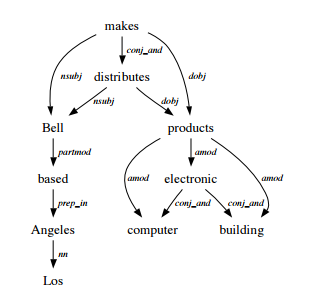
\includegraphics[scale=0.8]{dependency_tree}\end{center}
\caption[Strom vzťahov]{Strom vzťahov}\label{fig:dependency_tree}
\end{figure}

V tomto orientovanom stromovom grafe jednotlivé slová vety predstavujú vrcholy, pričom prechody medzi vrcholmi, hrany, reprezentujú vzťahy medzi nimi.

Ďalšia reprezentácia vzťahov zapisuje vzťahy priamo do vety. Na obrázku \fullref{fig:dependencies_in_sentence} vidíme, že medzi slovami \textit{She} a \textit{looks} je vzťah \textbf{nsubj} - nominal subject, medzi \textit{looks} a \textit{beautiful} je vzťah \textbf{acomp} - adjevtival complement, a v neposlednom rade medzi slovami \textit{very} a \textit{beautiful} je vzťah \textbf{advmod} - adverb modifier~\cite{StanfordDepManual}.
%, ktorý je nominálnou frázou, ktorý je syntaktický subjekt vety. Nadradená časť vo vzťahu nominal subject, tomto prípade \textit{She}, nemusí byť vždy sloveso. Ak je sloveso sponové sloveso, napríklad stať sa, tak koreňom vety je doplnok sponového slovesa, ktoré môže byť prídavné meno alebo podstatné meno.

\begin{figure}[H]
\begin{center}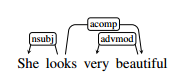
\includegraphics[scale=0.8]{dependencies_in_sentence}\end{center}
\caption[Vzťahy vo vete]{Vzťahy vo vete}\label{fig:dependencies_in_sentence}
\end{figure}

%
% Nástroje na spracovanie prirodzeného jazyka
%
\ifthenelse {\boolean{bachelor}}
{
	%\subsection{Subsection}
	\subsection{Nástroje na spracovanie prirodzeného jazyka}
}
{
	%\section{Subsection}
	\section{Nástroje na spracovanie prirodzeného jazyka}
}
\label{subsec:nlp_nastroje}
V súčastnosti je vyvinutých alebo sú vo vývoji viacero nástrojov, ktoré sa dajú použiť pri spracovávaní prirodzeného jazyka. Vývoj takýchto nástrojov je podporovaný na známych univerzitách ako sú napríklad Princeton, Stanford alebo Camridge, ale samozrejme svoje slovo tu má aj velikán Google. Pozrieme sa bližšie na niektoré z týchto nástrojov, čo ponúkajú a ako sa dajú využiť.

%
% WordNet
%
\ifthenelse {\boolean{bachelor}}
{
	%\subsection{Subsection}
	\subsubsection{WordNet}
}
{
	%\section{Subsection}
	\subsection{WordNet}
}
\label{subsubsec:wordnet}
WordNet je databáza anglických slov vyvíjaná na Princetonskej univerzite. Databáza obsahuje podstatné mena, prídavné mená, slovesá a príslovky, ktoré sú zatriedené do synonymických sád, synsetov~\cite{WordNetPage}.

Slová do synetov sú zaraďované podľa významu. To znamená, že slová auto a automobil, ktoré sú pre svoj význam zameniteľné vo vete, sa zaradujú do rovnakého synsetu. WordNet v súčastnosti (r. 2015) obsahuje 117 000 synsetov. Každý z týchto sysnsetov taktiež obsahuje krátku ukážku použitia slova~\cite{WordNetPage}.

Vo WordNet-e sa nachádzajú aj vzťahy medzi slovami v zmysle nadradenosti. Tým sa myslí, že stolička je nábytok a nábytok je fyzická vec a takto to pokračuje až po najvyššie slovo, od ktorého ,,dedia'' všetky - entita (viď. obrázok \fullref{fig:wordnet_relations}. Okrem vzťahu nadradenosti WordNet obsahuje aj vzťah zloženia. Stolička sa skladá z operadla a nôh. Toto zloženie je typické len konkrétne slovo a neprenáša sa hore stromom nadradenosti,   lebo pre stoličku je typické, že sa skladá z operadla a nôh, ale to už nie je typické pre nábytok.
Prídavné mená obsahujú aj vzťah antonymity, takže slovo \textit{suchý} bude prepojené so slovom \textit{mokrý} ako so svojím antonymom~\cite{WordNetPage}.

Tento nástroj je dostupný vo webovej verzií (viď. obrázok \fullref{fig:wordnet_search}), ale ponúka aj stiahnutie jeho databázových súborov, ktoré sa po splnení licenčných požiadaviek dajú využívať v projektoch.

\begin{figure}[H]
\begin{center}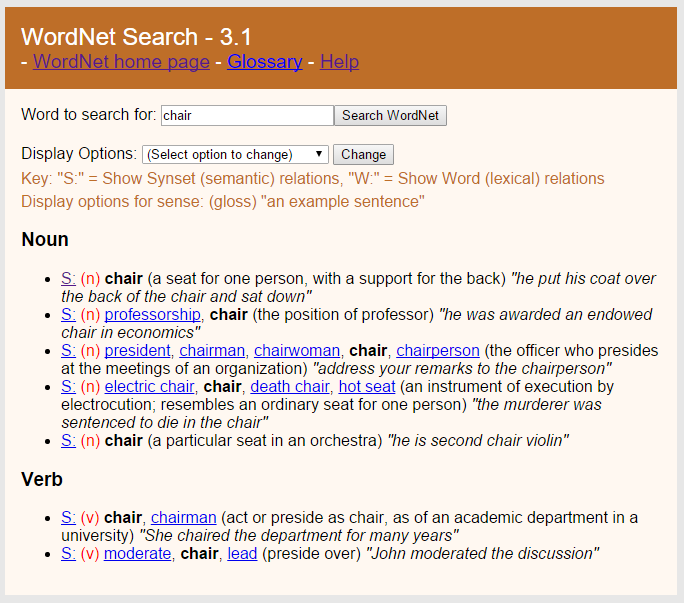
\includegraphics[scale=0.48]{wordnet_search}\end{center}
\caption[Webové rozhranie]{Webové rozhranie}\label{fig:wordnet_search}
\end{figure}

\begin{figure}[H]
\begin{center}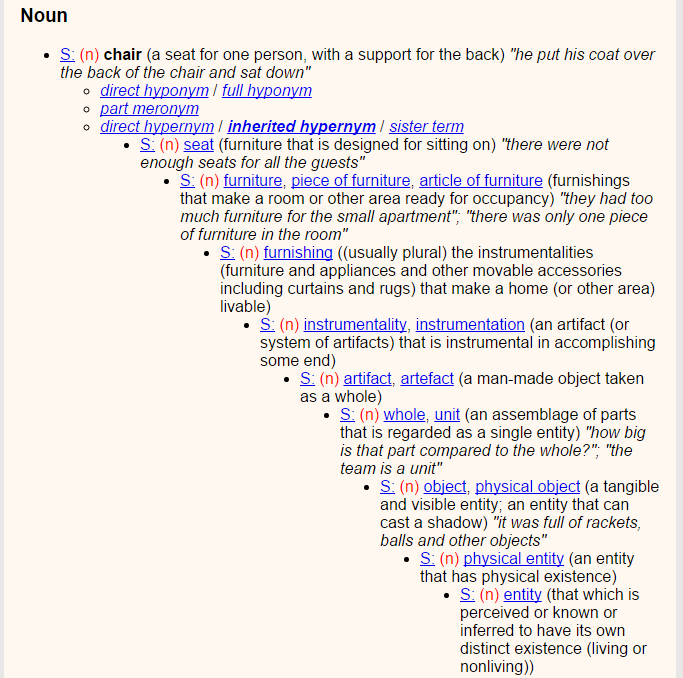
\includegraphics[scale=0.48]{wordnet_search_relations}\end{center}
\caption[Nadradenosť slov]{Nadradenosť slov}\label{fig:wordnet_relations}
\end{figure}

%
% StanfordNLP
%
\ifthenelse {\boolean{bachelor}}
{
	%\subsection{Subsection}
	\subsubsection{StanfordNLP}
}
{
	%\section{Subsection}
	\subsection{StanfordNLP}
}
\label{subsubsec:stanfordnlp}
Nástroj StanfordNLP je vyvíjaný na Stanfordskej univerzite. Skladá sa z niekoľkých softvérov, ktoré sa zameriavajú na úlohy spracovania prirodzeného jazyka popísané v sekcií \fullref{subsec:nlp}. Sú to softvéry \textit{Stanford Parser}, \textit{Stanford POS Tagger}, \textit{Stanford EnglishTokenizer}, \textit{Stanford Relation Extractor} a mnoho ďalších. \textit{Stanford CoreNLP} zahŕňa viacero z týchto softvérov, a práve tento nástroj budeme používať pri spracovaní učebných textov.

Nástroje StanfordNLP sú implementované v Jave, ale sú dostupné aj v iných programovacích jazykoch ako C\#, PHP alebo Python.

Dostupne je aj online webové demo. Na obrázku \fullref{fig:stanfordnlp_online_demo} vidíme výstupy z nástrojov ponúkaných balíkom StanfordNLP pre jednoduchý vstupný text skladajúci sa z jednej vety ,,Martin Nemček is a student at Slovak University of Technology in Bratislava.''.

\begin{figure}[H]
\begin{center}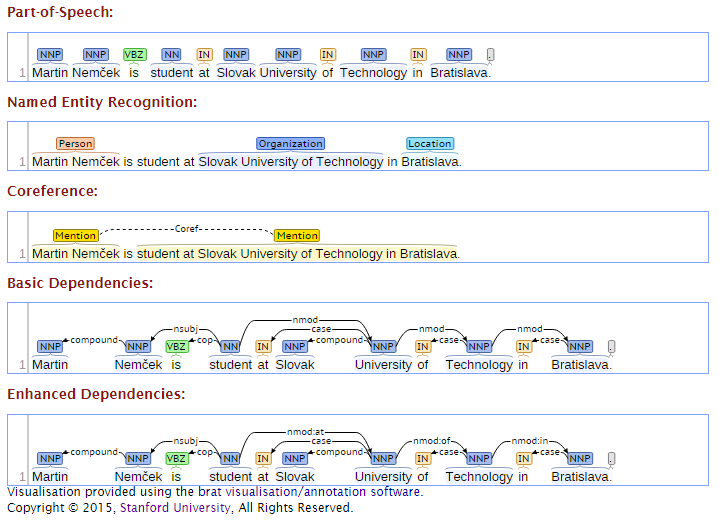
\includegraphics[scale=0.48]{stanfordnlp_online}\end{center}
\caption[StanfordNLP online demo]{StanfordNLP online demo}\label{fig:stanfordnlp_online_demo}
\end{figure}

%
% CambridgeAPI
%
\ifthenelse {\boolean{bachelor}}
{
	%\subsection{Subsection}
	\subsubsection{CambridgeAPI}
}
{
	%\section{Subsection}
	\subsection{CambridgeAPI}
}
\label{subsubsec:cambridgeapi}
CambridgeAPI je vytvorený na Cambridge univerzite. Umožňuje prístup k viacerým rôznym slovníkom. Momentálne tento nástroj ponúka prístup k pätnástim prekladovým slovníkom ako napríklad anglicko-čínsky, anglicko-ruský, anglicko-arabský, anglicko-japonský a ďalšie. Všetky prekladové slovníky majú primárny jazyk angličtinu. Slovenčinu v súčastnosti nepodporuje.

Spomínaný nástroj funguje na princípe dopytovania pomocou HTTP protokolu. Na obdržanie korektnej odpovede je potrebné mať osobný API kľúč. Ten sa dá získať kontaktovaním správcov CambridgeAPI.

%
% Google Ngram
%
\ifthenelse {\boolean{bachelor}}
{
	%\subsection{Subsection}
	\subsubsection{Google Ngram}
}
{
	%\section{Subsection}
	\subsection{Google Ngram}
}
\label{subsubsec:googlengram}
Google Ngram je postavený na ďalšom softvéry tohto giganta, Google Books. V knihách,  napísaných od roku 1500 až do súčastnosti, vyhľadáva výskyty n-gramov. Podporuje len niektoré jazyky, ako angličtina, francúzština, ruština, čínština. Na vyhľadávanie v knihách využíva optické rozoznávanie textu, pričom dokáže spracovať aj regulárne výrazy, avšak tie môžu byť použité iba ako náhrada celého slova, ale nie uprostred slova. Slovné spojenie ,,* Einstein'' spracuje, pričom ,,Albert Einste*n'' nie.

N-gram je podľa oxfordského slovníka definovaný ako postupnosť \textit{n} za sebou idúcich slov alebo znakov. \textit{Martin} je n-gram veľkosti jedna, 1-gram alebo unigram. \textit{Martin Nemček} je n-gram veľkosti dva, 2-gram alebo bigram a tak ďalej, pričom \textit{n} môže byť ľubovolné kladné, celé číslo.

Google Ngram Viewer poskytuje vizualizáciu vyhľadaných dát. Je dostupný vo webovom rozhraní. Na obrázku \fullref{fig:googlengram_visualization} vidno vizualizáciu výskytu mien \textit{Albert Einstein,Sherlock Holmes,Frankenstein} v knihách od roku 1800 do roku 2000.

\begin{figure}[H]
\begin{center}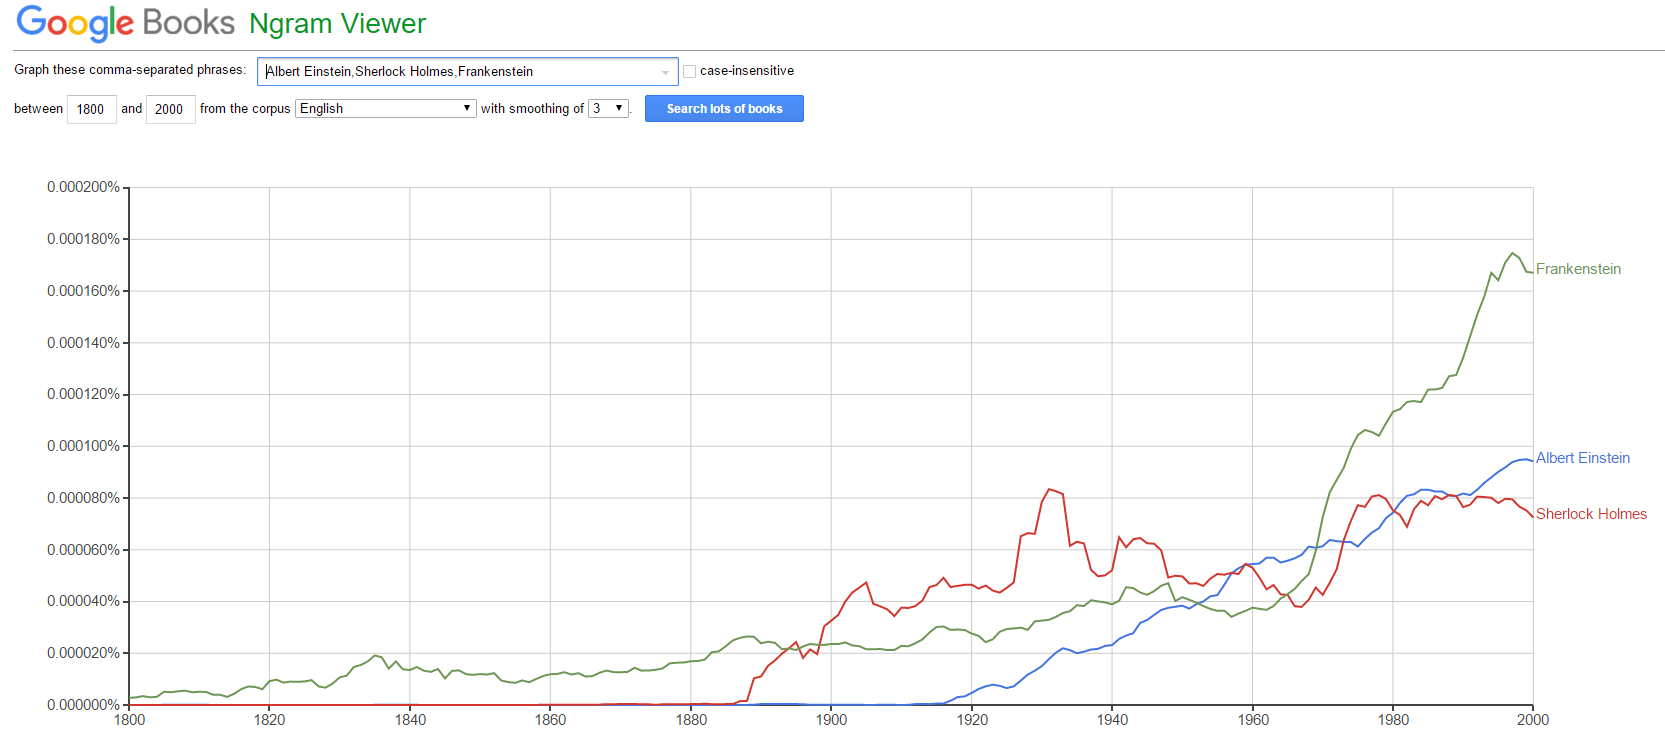
\includegraphics[scale=0.38]{googlengram_visualization}\end{center}
\caption[Google Ngram Viewer]{Google Ngram Viewer}\label{fig:googlengram_visualization}
\end{figure}

Tento nástroj okrem iného ponúka aj surové (angl. raw) dáta na stiahnutie.

%
% AlchemyAPI
%
\ifthenelse {\boolean{bachelor}}
{
	%\subsection{Subsection}
	\subsubsection{AlchemyAPI}
}
{
	%\section{Subsection}
	\subsection{AlchemyAPI}
}
\label{subsubsec:alchemyapi}
AlchemiAPI obsahuje dvanásť funkcií, z ktorých sú niektoré zamerané na úlohy spracovania prirodzeného jazyka popísané v sekcií \fullref{subsec:nlp}, ako napríklad extrakcia entít, extrakcia kľúčových slov, extrakcia vzťahov, ale aj iné zaujímave funkcie, napríklad extrakcia autora z textu.

Na používanie tohto nástroja je potrebné sa zaregistrovať pre obdržanie API kľúču. S týmto kľúčom je tisíc dopytov denne zdarma. Dostupnosť v programovacích jazykoch je široká, kedže ponúka knižnicu v deviatich najpoužívanejších programovacích jazykoch.

Pre AlchemyAPI je dostupné aj online webové demo, viď obrázok \fullref{fig:alchemyapi_visualization}, kde je vidno širokú ponuku, ktorú tento nástroj ponúka.

\begin{figure}[H]
\begin{center}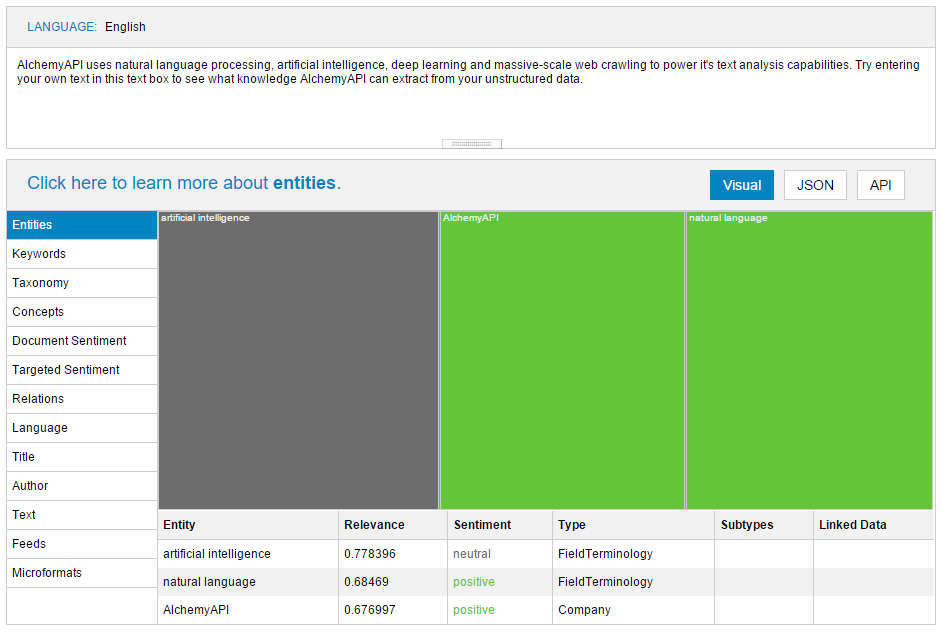
\includegraphics[scale=0.48]{alchemyapi_visualization}\end{center}
\caption[AlchemyAPI online demo]{AlchemyAPI online demo}\label{fig:alchemyapi_visualization}
\end{figure}

Dáta sú vo formáte JSON a okrem spracovania prirodzeného jazyka AlchemyAPI ponúka aj nástroje na extrahovanie obsahu z obrázku alebo rozpoznávanie tvári na obrázkoch.

%
% Aplikácie na spracovanie prirodzeného jazyka
%
\ifthenelse {\boolean{bachelor}}
{
	%\subsection{Subsection}
	\subsection{Aplikácie na spracovanie prirodzeného jazyka}
}
{
	%\section{Subsection}
	\section{Aplikácie na spracovanie prirodzeného jazyka}
}
Dostupnosť aplikácií na spracovanie prirodzeného jazyka je veľká a široká. Najväčší podiel tvoria aplikácie zamerané na preklad. V tejto kapitole si prestavíme niektorých predstaviteľov tejto kategórie aplikácií.

%
% InterText
%
\ifthenelse {\boolean{bachelor}}
{
	%\subsection{Subsection}
	\subsubsection{InterText}
}
{
	%\section{Subsection}
	\subsection{InterText}
}
InterText\footnote{http://wanthalf.saga.cz/intertext} je editor paralelne zarovnaných textov, využívaný na správu viacerých paralelne zarovnaných verzií textu rôznych jazykov na úrovni viet. Táto aplikácia je dostupná vo verzií pre desktop, ale aj pre server.

Podporuje viacero formátovaní textu, či už čistý (angl. plain) text alebo XML a taktiž zobrazuje aj HTML značky. Riadky obsahujú vety oddelené znakom konca riadku a sú očíslované. Umožňuje funkcie ako presúvanie riadkov textu alebo zoskupenie viacerých do jedného, krok vpred a vzad. V spracovávanom texte sa dá vyhľadávať a je možné tento text aj upraviť podľa vlastných potrieb.

InterText nezohľadňuje používateľove úpravy textu počas používanie a pri následnom spracovávaní textu sa tak neprispôsobí používateľovi. Okrem toho jeho náplň sa nedá pokladať za zjednodušovanie textu. 

Na obrázku~\fullref{fig:intertext_interface} je zobrazená aplikácia InterText s testovacím vstupom, na ktorom je vidno väčšinu, už spomenutej, funkcionality, ako presúvanie a zoskupovanie riadkov, číslovanie, atď.

\begin{figure}[H]
	\begin{center}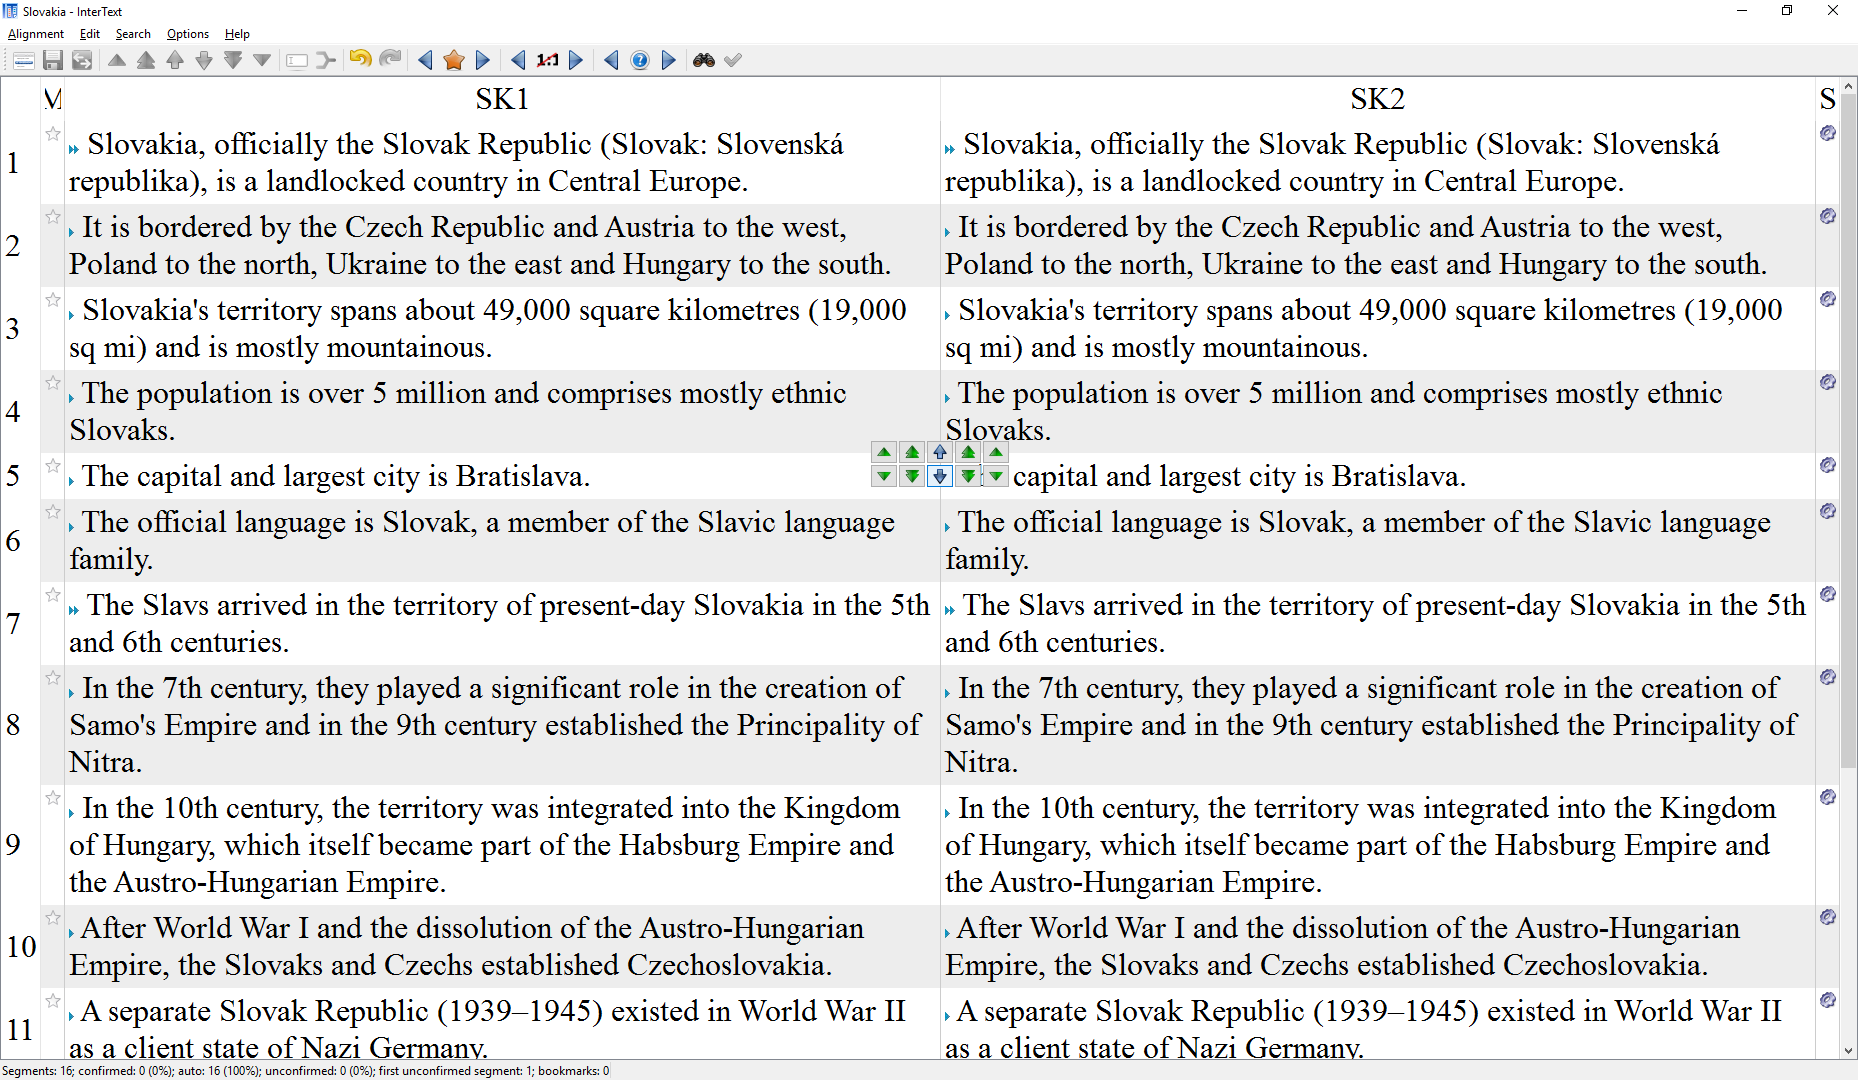
\includegraphics[scale=0.33]{intertext_interface}\end{center}
	\caption[Aplikácia InterText]{Aplikácia InterText}\label{fig:intertext_interface}
\end{figure}

%
% NOVA Text Aligner
%
\ifthenelse {\boolean{bachelor}}
{
	%\subsection{Subsection}
	\subsubsection{NOVA Text Aligner}
}
{
	%\section{Subsection}
	\subsection{NOVA Text Aligner}
}
NOVA Text Aligner\footnote{http://www.supernova-soft.com/wpsite/products/text-aligner/} je aplikácia na zarovnávanie textu, pričom nevyužíva algoritmy na zarovnávanie textu, ale manuálne používateľovo určovanie zarovnania.

Ako vidno na obrázku~\fullref{fig:nova_text_aligner_interface} hlavná editovacia časť aplikácie je rozdelené do dvoch častí. Umožňuje do ľavej aj pravej časti načítať rôzny text, v ktorom sa dá veľmi jednoducho vyhľadávať, k čomu napomáha zvýraznenie vyhľadaných slov. Načítaný text je možné premiestňovať a zoskupovať, či už podľa riadkov alebo aj v celých blokoch a nechýba možnosť editovať text. Je možné si túto aplikáciu prispôsobiť. Ponúka možnosti ako zmena typ písma a pod. Finálny, spracovaný text sa dá exportovať do viacerých formátov, z ktorých populárne sú formáty elektronických knižiek EPUB a MOBI.

Aplikácia je zameraná hlavne na usporadúvanie textu, nezaznamenáva si používateľove zmeny textu a neprispôsobuje sa podľa toho pri ďalšom použití, funguje iba lokálne. NOVA Text Aligner je dostupná iba v skúšobnej verzií, pre dlhodobé používanie si treba zakúpiť licenciu.

\begin{figure}[H]
	\begin{center}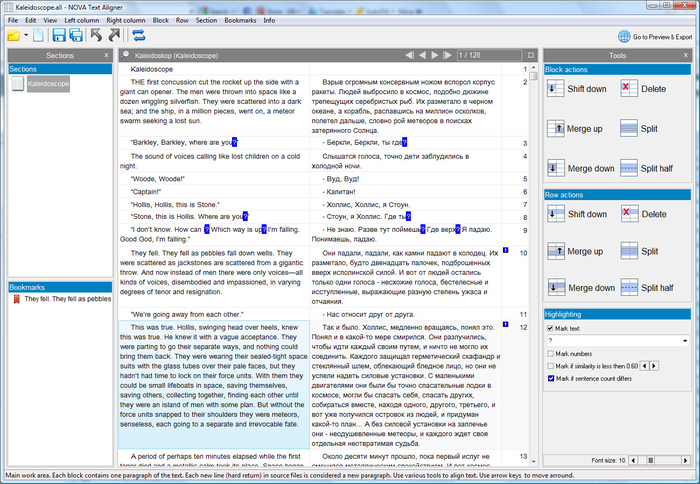
\includegraphics[scale=0.56]{nova_text_aligner_interface}\end{center}
	\caption[Aplikácia NOVA Text Aligner]{Aplikácia NOVA Text Aligner\footnotemark}\label{fig:nova_text_aligner_interface}
\end{figure}
\footnotetext{http://parallel-text-aligner.en.softonic.com/}

%
% LF Aligner
%
\ifthenelse {\boolean{bachelor}}
{
	%\subsection{Subsection}
	\subsubsection{LF Aligner}
}
{
	%\section{Subsection}
	\subsection{LF Aligner}
}
Aplikácia LF Aligner je zameraná na spracovanie textu rôznych jazykov. Ponúka možnosť použiť až 99 jazykov, čo ale znamená 99 vstupných súborov, každý so zvoleným jazykom. Dokáže spracovať rôzne typy vstupných súborov od čistého textu, PDF súborov, cez URL stránok s textom až po správy Európskeho parlamentu, ktoré automaticky stiahne. Výstup môže byť taktiež viacerých druhov, napríklad cez grafické rozhranie LF Aligner alebo vygenerovanie XLS súboru. Na obrázku~\fullref{fig:lf_aligner_interface} vidno grafické rozhranie tejto aplikácie, ktoré ponúka mnohé vymoženosti. Samozrejme je možné premiestňovať a zoskupovať riadky, doplnenie ďalšieho súboru na spracovávanie, uloženie zmien súboru prepísaním jeho dát a mnohé ďalšie.

\begin{figure}[H]
	\begin{center}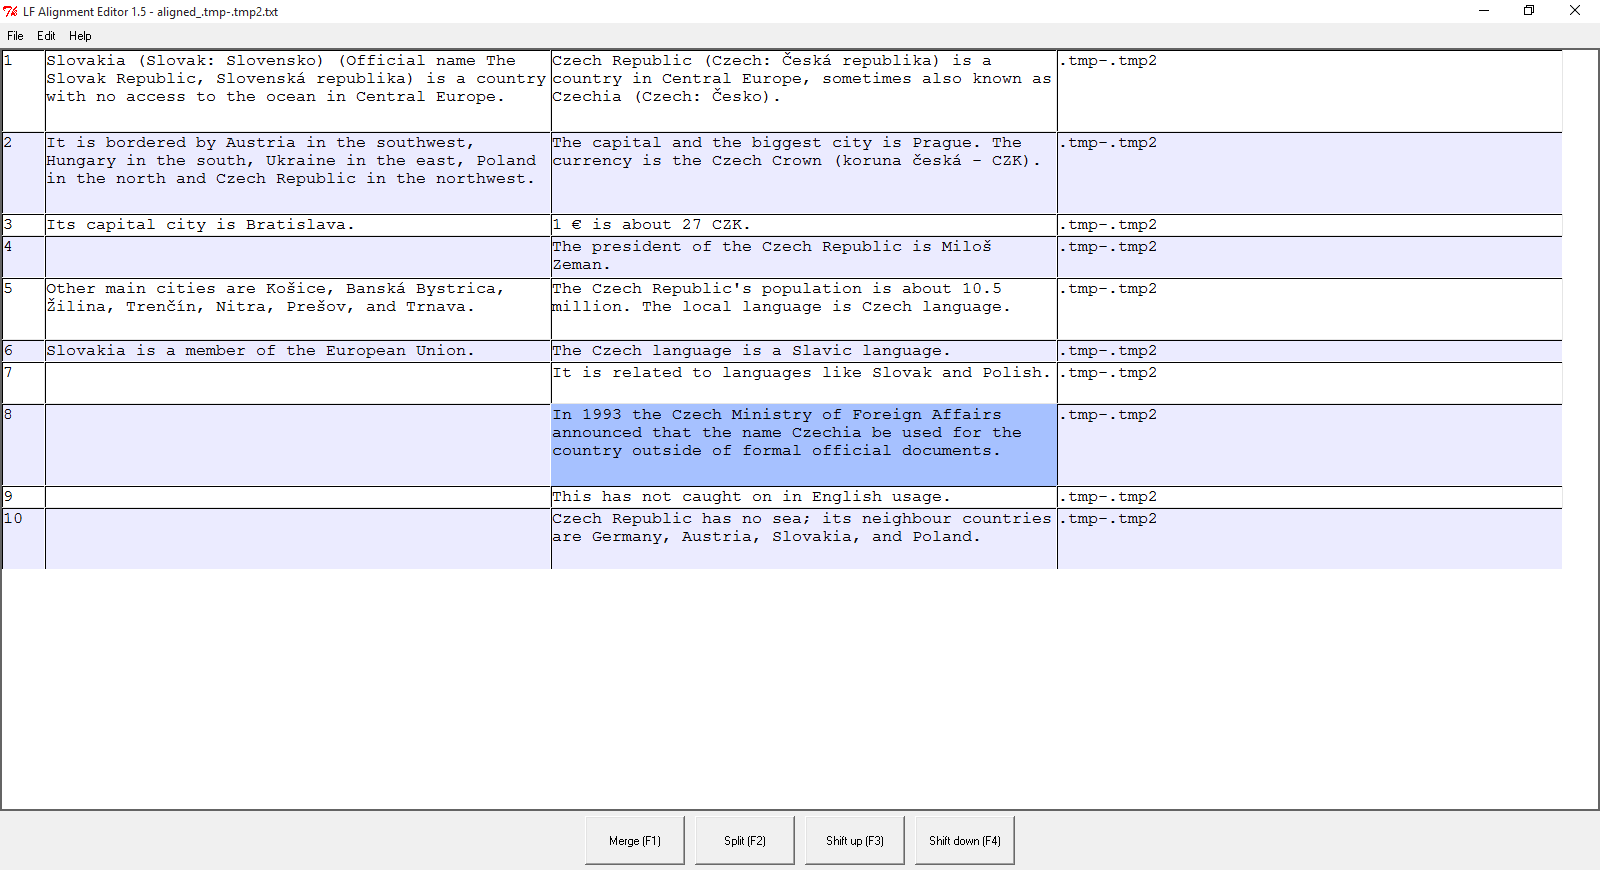
\includegraphics[scale=0.33]{lf_aligner_interface}\end{center}
	\caption[Aplikácia LF Aligner]{Aplikácia LF Aligner}\label{fig:lf_aligner_interface}
\end{figure}
\footnotetext{http://parallel-text-aligner.en.softonic.com/}

%
% Zhrnutie aplikácií na spracovanie prirodzeného jazyka
%
\ifthenelse {\boolean{bachelor}}
{
	%\subsection{Subsection}
	\subsubsection{Zhrnutie}
}
{
	%\section{Subsection}
	\subsection{Zhrnutie}
}
Všetky analyzované aplikácie sú užitočné vo svojom obore, ale ani jedna nespĺňa všetky požiadavky na systém schopný spoznámkovať učebný text v takom rozsahu, ktorý by umožňoval používateľovi prispôsobiť si spracovaný text. Systém musí vedieť prispôsobovať svoje spracovanie textu podľa používateľových úprav a ponúkať mu k tomu vhodné rozhranie. Takisto musí ukladať dáta mimo používateľovho úložného priestoru.

%
% Smerovanie práce
%
\ifthenelse {\boolean{bachelor}}
{
	%\section{Analysis}
	\section{Smerovanie práce} 
}
{
	%\chapter{Analysis}
	\chapter{Smerovanie práce}
}
V letnom semestri plánujem dokončiť prototyp. To znamená, spraviť používateľské rozhranie, ktoré bude umožňovať vložiť text na spracovanie, zobrazí poznámky a tak isto umožní používateľovi pre ľubovolnú vetu pozmeniť tvar poznámky poznámky. Tieto zmeny sa uložia do databázy a zohľadnia pri ďalšom použití.

Okrem dokončenia prototypu plánujem napísať všetky potrebné kapitoly a dokončiť tým celú prácu.

%
% Opis prototypu
%
\ifthenelse {\boolean{bachelor}}
{
	%\section{Analysis}
	\section{Opis prototypu} 
}
{
	%\chapter{Analysis}
	\chapter{Opis prototypu}
}
V zimnom semestri som implementoval prototyp aplikácie na spoznámkovanie učebného textu.

%
% Notenizer
%
\ifthenelse {\boolean{bachelor}}
{
	%\section{Analysis}
	\subsection{Notenizer} 
}
{
	%\chapter{Analysis}
	\section{Notenizer}
}
\label{subsection:notenizer}
\textbf{Notenizer} je prototyp aplikácie na extrahovanie relevantných informácií z učebných textov. Využíva nástroj Stanford CoreNLP, ktorý je implementovaný v Jave, ale cez IKVM je portnutý aj na C\#. Na ukážke \fullref{code:spustenie_stanford_corenlp} je ukázané prepojenie nástroja StanfordCoreNLP s aplikáciou Notenizer. 
\\

\begin{lstlisting}[ language = csharp, caption={Spustenie StanfordCoreNLP}, label = {code:spustenie_stanford_corenlp}]
String jarRoot = @"stanford-corenlp-3.5.2-models";

Properties properties = new Properties();
// Zvolime, ktore nastroje chceme pouzit.
// pos = part-of-speech tagger
// ssplit = sentence split
// atd.
properties.setProperty("annotators", "tokenize, ssplit, pos, parse");
properties.setProperty("sutime.binders", "0");
properties.setProperty("ner.useSUTime", "false");

// Nastavenie aktualneho priecinku, aby StanfordCoreNLP vedel najst
// vsetky potrebne subory
String currentDirectory = Environment.CurrentDirectory;
Directory.SetCurrentDirectory(jarRoot);
StanfordCoreNLP pipeline = new StanfordCoreNLP(properties);
Directory.SetCurrentDirectory(currentDirectory);

// Vytvorenie anotacie z textu
Annotation annotation = new Annotation(text);

// Spustenie
pipeline.annotate(annotation);
\end{lstlisting}

Údaje získane z tohto nástroja, napríklad POS značky, vzťahy medzi slovami, pozície slov a mnoho ďalších, Notenizer ďalej spracováva. Najdôležitejšie vlastnosti, ktoré sa využívajú v najväčšej miere pri spracovávaní sú závislosti (angl. dependency) medzi slovami vo vete.  

Spracovávaný text sa postupne spracováva po vetách. Každá veta sa samostatne ,,rozparsuje'', spoznámkuje. Vety sa parsujú na základe pravidiel. Na začiatku je daná statická sada pravidiel na spracovanie viet a textov. Po tom, ako sa celý text spracuje, tak sa použité pravidlá uložia do databázy aj s informáciami o pôvodnej vete a novo vytvorenej, zjednodušenej vete. Následne pri opätovnom používaní aplikácie, keď sa začne spracovávať text, tak sa vyhľadajú pre každú vetu pravidlá v databáze, vyberú sa tie s najväčšou zhodou a podľa toho sa spracuje daná veta. Statické pravidla na spracovanie vety sa v tomto prípade použijú len v prípade, ak v sa v databáze nenašli žiadne pravidlá na spracovanie vety, ktoré by pre danú vetu vyhovovali, to znamená, že takúto alebo podobnú vetu zatiaľ Notenizer nespracovával.

Na obrázku~\fullref{fig:example_output} je ukázaný ukážkový výstup prototypu pre vstupný text z wikipédie:
\textit{Czech Republic (Czech: Česká republika) is a country in Central Europe, sometimes also known as Czechia (Czech: Česko). The capital and the biggest city is Prague. The currency is the Czech Crown (koruna česká - CZK). 1€ is about 27 CZK. The president of the Czech Republic is Miloš Zeman. The Czech Republic's population is about 10.5 million. The local language is Czech language. The Czech language is a Slavic language. It is related to languages like Slovak and Polish. In 1993 the Czech Ministry of Foreign Affairs announced that the name Czechia be used for the country outside of formal official documents. This has not caught on in English usage. Czech Republic has no sea; its neighbour countries are Germany, Austria, Slovakia, and Poland.}
\\

Výstup je v tvare [pôvodná veta] ===>> [poznámka z pôvodnej vety].

\begin{figure}[H]
\begin{center}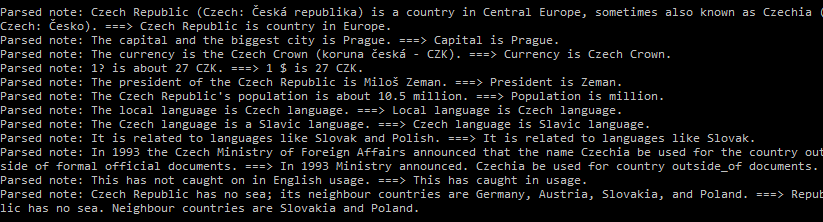
\includegraphics[scale=0.7]{example_output}\end{center}
\caption[Ukážkový výstup prototypu]{Ukážkový výstup prototypu}\label{fig:example_output}
\end{figure}

%
% Pravidlá
%
\ifthenelse {\boolean{bachelor}}
{
	%\subsection{Subsection}
	\subsubsection{Pravidlá}
}
{
	%\section{Subsection}
	\subsection{Pravidlá}
}
\label{subsubsec:notenizer_pravidla}
Pri spracovaní pôvodnej vety sa na túto vetu aplikuje \textit{pravidlo na spracovanie}. Toto pravidlo obsahuje okrem iného zoznam závislostí slov vo vete. Podľa týchto závislostí slov vo vete sa v spracovávanej vete vyhľadajú slová, ktoré majú byť použité v poznámke. Vyhľadávajú sa, okrem iného, podľa POS značiek a indexov vo vete.

%
% Ukladanie a hodnoty pravidiel
%
\ifthenelse {\boolean{bachelor}}
{
	%\subsection{Subsection}
	\subsubsection{Ukladanie a hodnoty pravidiel}
}
{
	%\section{Subsection}
	\subsection{Ukladanie a hodnoty pravidiel}
}
\label{subsubsec:notenizer_ukldanie_a_hodnoty_pravidiel}
Po spracovávaní sa do databázy uložia použité pravidla aj s ostatnými informáciami o pôvodnej a novej vete. Ukladá sa 
\begin{itemize}
	\item Hodnota pôvodnej a novej vety
	\item Zoznam indexov slov, za ktorými bola v poznámke ukončená veta (ak pôvodná veta je súvetie, tak z nej môže vzniknúť viacero poznámok)
	\item Všetky závislostí slov v pôvodnej vete
	\item Všetky závislosti slov v poznámke
\end{itemize}
pričom každá závislosť slov vo vete sa skladá z 
\begin{itemize}
	\item Názvu závislosti
	\item Hodnota governora závislosti
	\item Hodnota dependenta závislosti
	\item Pozícia závislosti vo vete
	\item POS značka a index slova pre governora aj dependenta
\end{itemize}

%
% Vyhľadanie pravidla
%
\ifthenelse {\boolean{bachelor}}
{
	%\subsection{Subsection}
	\subsubsection{Vyhľadanie pravidla}
}
{
	%\section{Subsection}
	\subsection{Vyhľadanie pravidla}
}
\label{subsubsec:notenizer_vyhladanie_pravidla}
Pri spracovávaní vety sa v prvom kroku pozrie do databázy a vyhľadá sa pravidlo na spracovanie tejto vety. Pravidlo sa v databáze vyhľadáva podľa nasledovných podmienok.
\begin{enumerate}
	\item Počet závislostí vety
	\item Názvy závislostí vety
\end{enumerate}
Veta v databáze, ktorej pravidlo chceme použiť, musí spĺňať tieto dve pravidlá. Musí mať rovnaký počet závislostí vo vete ako aktuálne spracovávaná veta a taktiež názvy všetkých závislostí musia sedieť.

Avšak pri týchto podmienkach môže nastať situácia, kedy pre aktuálne spracovávanú vetu bude vyhovovať viacero viet z databázy. V tomto prípade určujeme pravidlo vety s najväčšou zhodou a to sa následne aplikuje.
\\

Zistenie najväčšej zhody ma viacero krokov. Najskôr sa spočítavajú zhody POS značiek governerov a dependentov a indexy slov nezávisle od seba, čiže sa len zisťuje, či spracovávaná veta obsahuje závislosť s nejakou hodnotou indexu, alebo governora, atď.
V druhom kroku sa spočítavajú zhody POS značiek a zároveň aj indexov slov vo vete. To znamená, že sa zisťuje, či sa v spracovávanej vete nachádza napríklad závislosť, ktorej governor ma hodnotu \textit{car} a zároveň má index hodnotu 3.
V poslednom, treťom, kroku sa zisťuje, či sa závislosti zhodujú na všetkých hodnotách, čiže governor a jeho hodnota a index a dependent a jeho hodnota a index \textit{súčasne}.

Tieto tri hodnoty sa na záver spočítajú a tým získame percentuálne ohodnotenie zhody viet.


%%
%% analysis part 1
%%
\newpage
%
% Začiatok druhej časti analýzy
% Analýza nástrojov na správu paralelných textov
%
\ifthenelse {\boolean{bachelor}}
{
	%\section{Analysis}
	\section{Analýza nástrojov na správu paralelných textov} 
}
{
	%\chapter{Analysis}
	\chapter{Analýza nástrojov na správu paralelných textov}
}
Dostupnosť aplikácií na spracovanie prirodzeného jazyka je veľká a široká. Najväčší podiel tvoria aplikácie zamerané na preklad. My sa zameriame na aplikácie, ktoré umožňujú editovať paralelný text.

Nástroje na správu paralelných textov uľahčujú spracovanie viacerých druhov a verzií textu. Na jednej strane majú zdrojový text alebo súbor a na druhej strane výsledný text alebo súbor. Hlavný dôraz sa kladie práve na transformáciu zo zdrojového textu na cieľový. Transformácia môže mať viacero podôb, ako preklad, zarovnanie alebo zjednodušenie textu, a mnoho ďalších. Texty sú zväčša rozdelené podľa viet, pre zjednodušenie transformácie, pričom vety na jednej úrovni zvyčajne spolu súvisia podľa určitej vlastnosti.

V následujúcich častiach si predstavíme niektorých predstaviteľov tohto druhu nástrojov.

%
% InterText
%
\ifthenelse {\boolean{bachelor}}
{
	%\subsection{Subsection}
	\subsection{InterText}
}
{
	%\section{Subsection}
	\section{InterText}
}
InterText\footnote{http://wanthalf.saga.cz/intertext} je editor paralelne zarovnaných textov, využívaný na správu viacerých paralelne zarovnaných verzií textu rôznych jazykov na úrovni viet. Táto aplikácia je dostupná vo verzií pre desktop, ale aj pre server.

Podporuje viacero formátovaní textu, či už čistý (angl. plain) text alebo XML a taktiž zobrazuje aj HTML značky. Riadky obsahujú vety oddelené znakom konca riadku a sú očíslované. Umožňuje funkcie ako presúvanie riadkov textu alebo zoskupenie viacerých do jedného, krok vpred a vzad. V spracovávanom texte sa dá vyhľadávať a je možné tento text aj upraviť podľa vlastných potrieb.

InterText nezohľadňuje používateľove úpravy textu počas používania a pri následnom spracovávaní textu sa tak neprispôsobí používateľovi. Okrem toho zjednodušovanie textu v tomto nástroji by bolo pomerne náročné.

Na obrázku~\fullref{fig:intertext_interface} je zobrazená aplikácia InterText s testovacím vstupom, na ktorom je vidno väčšinu už spomenutej funkcionality, ako presúvanie a zoskupovanie riadkov, číslovanie, atď.

\begin{figure}[H]
	\begin{center}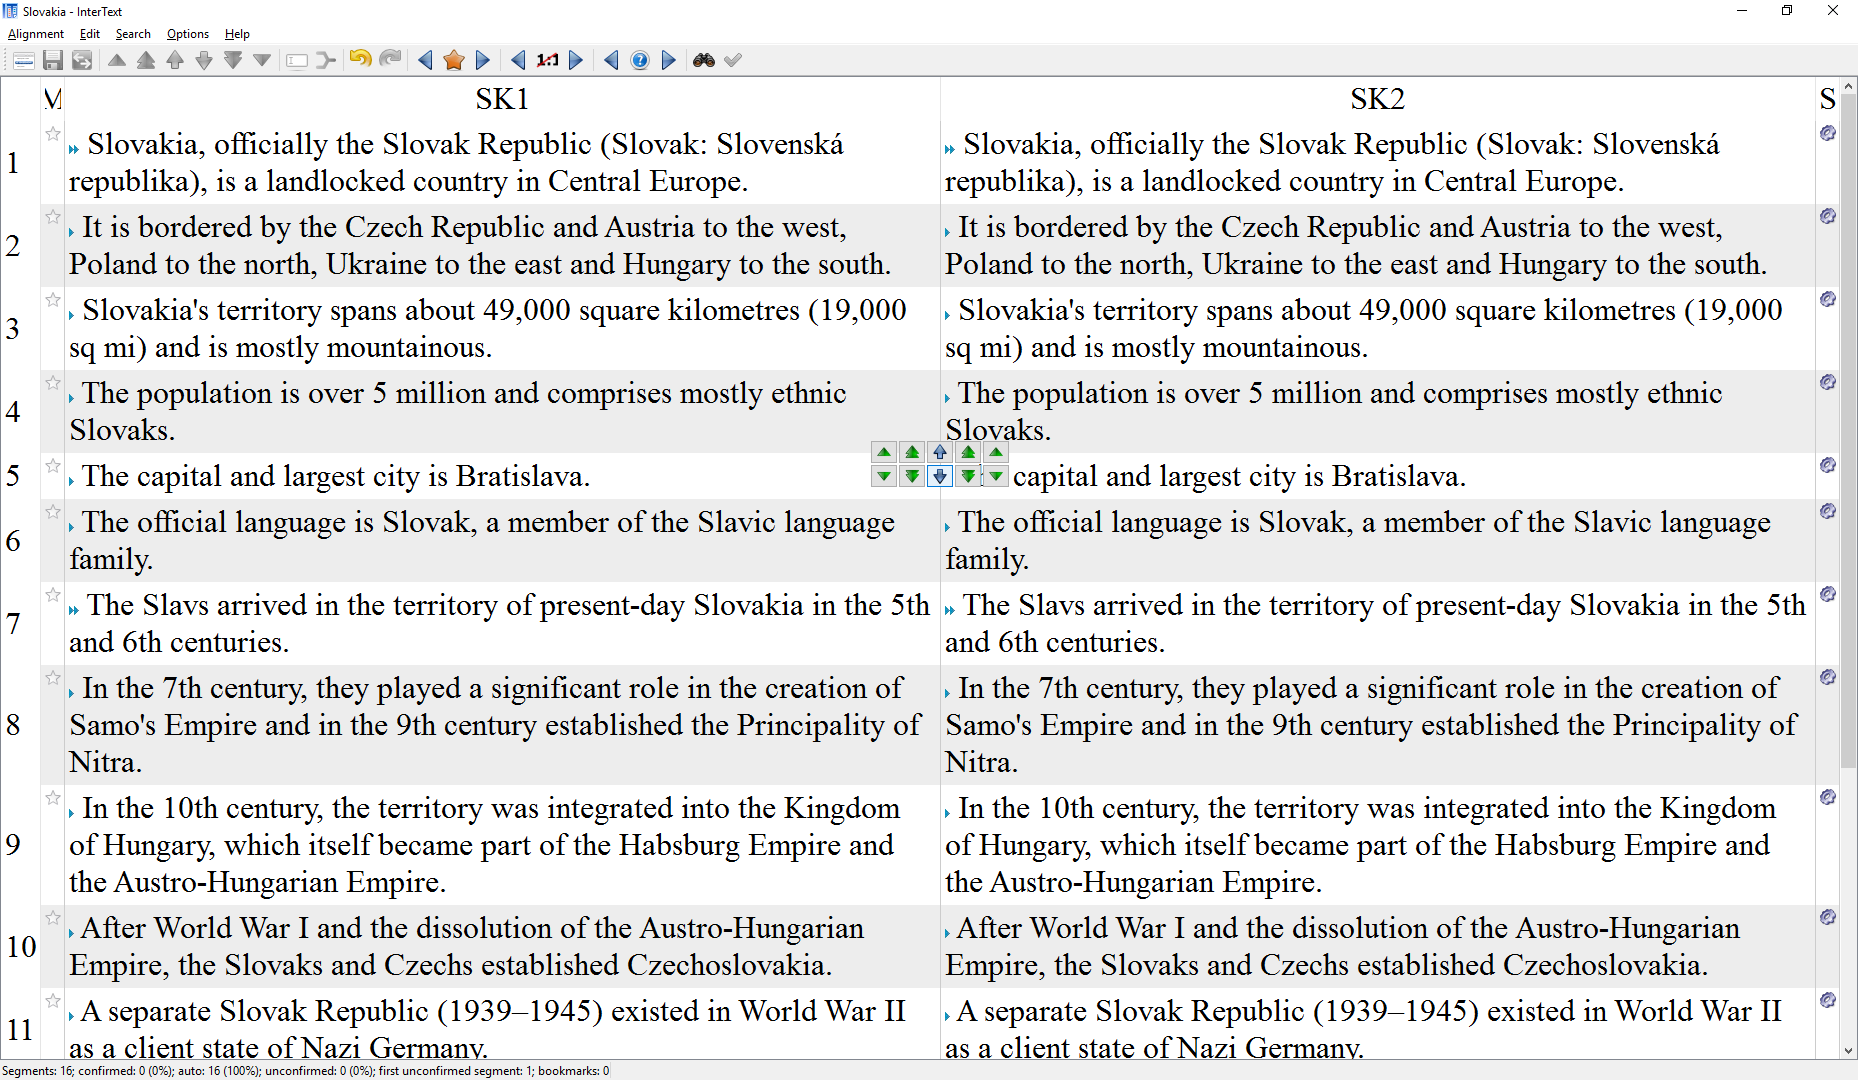
\includegraphics[scale=0.33]{intertext_interface}\end{center}
	\caption[Aplikácia InterText]{Aplikácia InterText}\label{fig:intertext_interface}
\end{figure}

%
% NOVA Text Aligner
%
\ifthenelse {\boolean{bachelor}}
{
	%\subsection{Subsection}
	\subsection{NOVA Text Aligner}
}
{
	%\section{Subsection}
	\section{NOVA Text Aligner}
}
NOVA Text Aligner\footnote{http://www.supernova-soft.com/wpsite/products/text-aligner/} je aplikácia na zarovnávanie textu, pričom nevyužíva algoritmy na zarovnávanie textu, ale používateľ si musí sám určiť zarovnanie.

Ako vidno na obrázku~\fullref{fig:nova_text_aligner_interface} hlavná editovacia časť aplikácie je rozdelené do dvoch častí. Umožňuje do ľavej aj pravej časti načítať rôzny text, v ktorom sa dá veľmi jednoducho vyhľadávať, k čomu napomáha zvýraznenie vyhľadaných slov. Načítaný text je možné premiestňovať a zoskupovať, či už podľa riadkov alebo aj v celých blokoch a nechýba možnosť editovať text. Je možné si túto aplikáciu prispôsobiť. Ponúka možnosti ako zmena typu písma a pod. Finálny spracovaný text sa dá exportovať do viacerých formátov, z ktorých populárne sú formáty elektronických knižiek EPUB a MOBI.

Aplikácia je zameraná hlavne na usporadúvanie textu, nezaznamenáva si používateľove zmeny textu a neprispôsobuje sa podľa toho pri ďalšom použití a funguje iba lokálne. NOVA Text Aligner je dostupná iba v skúšobnej verzií, pre dlhodobé používanie si treba zakúpiť licenciu.

\begin{figure}[H]
	\begin{center}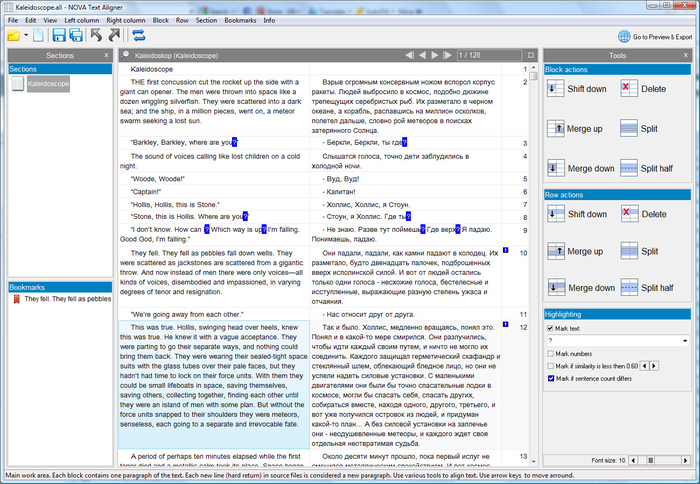
\includegraphics[scale=0.56]{nova_text_aligner_interface}\end{center}
	\caption[Aplikácia NOVA Text Aligner]{Aplikácia NOVA Text Aligner\footnotemark}\label{fig:nova_text_aligner_interface}
\end{figure}
\footnotetext{http://parallel-text-aligner.en.softonic.com/}

%
% LF Aligner
%
\ifthenelse {\boolean{bachelor}}
{
	%\subsection{Subsection}
	\subsection{LF Aligner}
}
{
	%\section{Subsection}
	\section{LF Aligner}
}
Aplikácia LF Aligner\footnote{www.sourceforge.net/projects/aligner} je zameraná na spracovanie textu rôznych jazykov. Ponúka možnosť použiť až 99 jazykov, čo ale znamená 99 vstupných súborov, každý so zvoleným jazykom. Dokáže spracovať rôzne typy vstupných súborov od čistého textu, PDF súborov, cez URL stránok s textom až po správy Európskeho parlamentu, ktoré automaticky stiahne. Výstup môže byť taktiež viacerých druhov, napríklad cez grafické rozhranie LF Aligner alebo vygenerovanie XLS súboru. Na obrázku~\fullref{fig:lf_aligner_interface} vidno grafické rozhranie tejto aplikácie, ktoré ponúka mnohé vymoženosti. Samozrejmosťou je možnosť premiestňovať a zoskupovať riadky, doplnenie ďalšieho súboru na spracovávanie, uloženie zmien súboru prepísaním jeho dát a mnohé ďalšie.

\begin{figure}[H]
	\begin{center}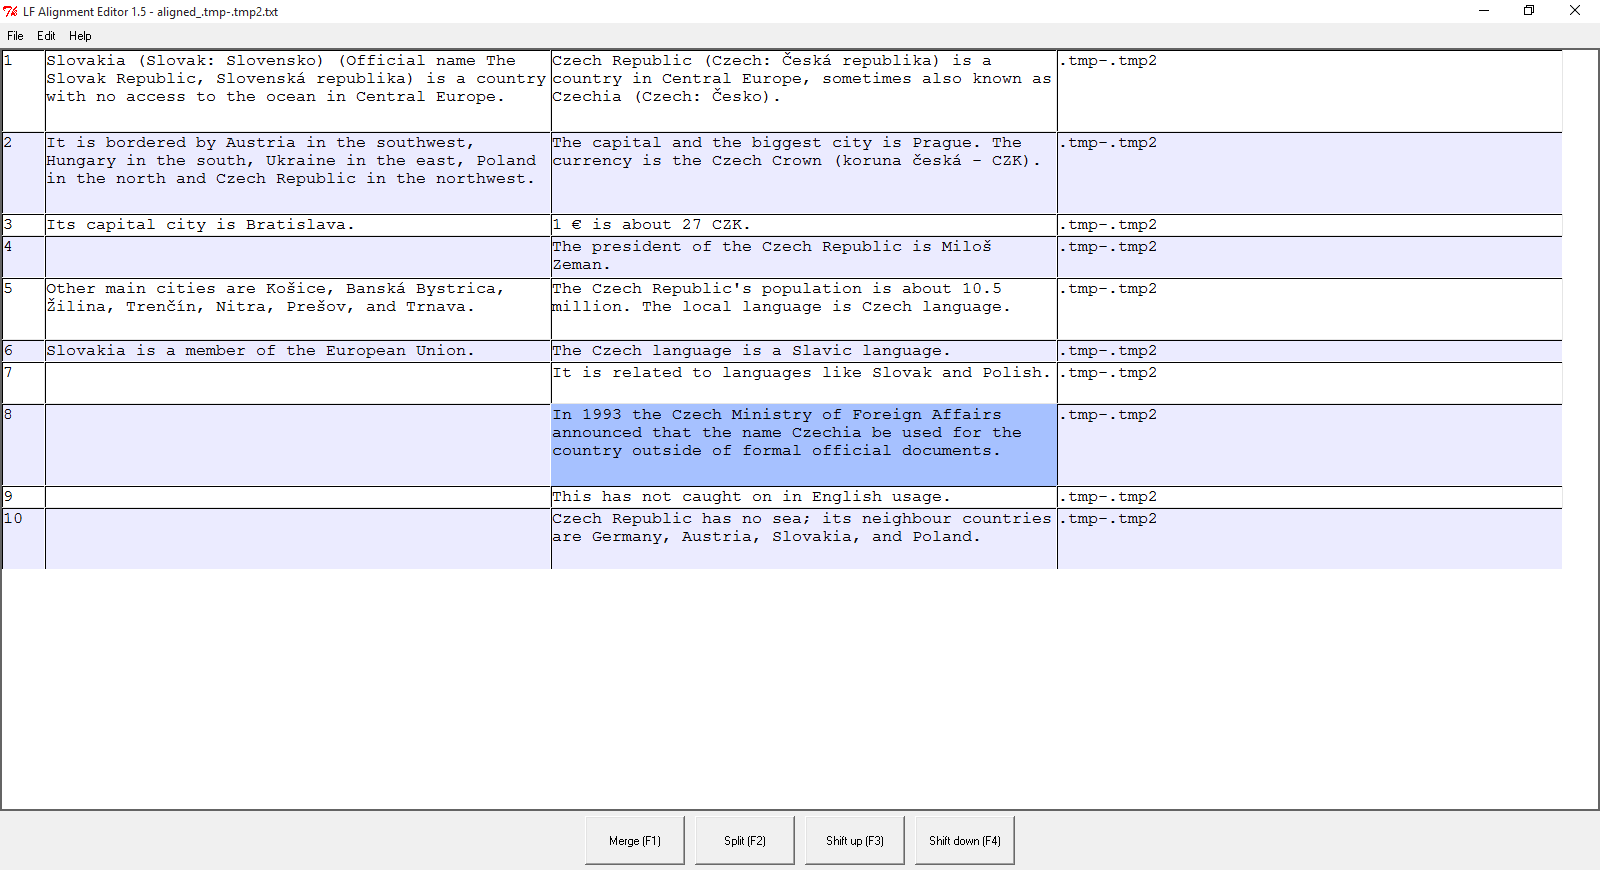
\includegraphics[scale=0.33]{lf_aligner_interface}\end{center}
	\caption[Aplikácia LF Aligner]{Aplikácia LF Aligner}\label{fig:lf_aligner_interface}
\end{figure}
\footnotetext{http://parallel-text-aligner.en.softonic.com/}

%
% Google Translate
%
\ifthenelse {\boolean{bachelor}}
{
	%\subsection{Subsection}
	\subsection{Google Translate}
}
{
	%\section{Subsection}
	\section{Google Translate}
}
Za najznámejšieho zástupcu webových nástrojov na spracovanie paralelných textov sa dá pokladať nástroj Google Translate\footnote{translate.google.com}. Využíva sa na preklad slov, viet, ale dokáže spracovať aj celé texty. Momentálne podporuje preklad z a do 91 jazykov. Dokáže rozpoznať a preložiť hovorenú reč aj písaný text. Pri preklade jednotlivých slov zobrazuje viacero možných prekladov do druhého jazyka, pričom pri preklade z anglického jazyka ponúka aj ukážky viet, v ktorých sa prekladané slovo môže použiť. Správnu výslovnosť preloženého aj prekladaného slova alebo textu, si používateľ môže vypočuť na krátkej zvukovej ukážke.

Na obrázku~\fullref{fig:google_translate_example} je zobrazený preklad anglického textu do slovenského. Vidno, že preklad do minoritných jazykov ešte nie je dokonalý.

\begin{figure}[H]
	\begin{center}
\includegraphics[scale=0.55]{google_translate_example}\end{center}
	\caption[Google Translate]{Google Translate}\label{fig:google_translate_example}
\end{figure}

Analyzované nástroje nespĺňajú všetky požiadavky na systém schopný spoznámkovať učebný text v takom rozsahu, ktorý by umožňoval používateľovi prispôsobiť si spracovaný text. Systém musí umožňovať editáciu jednotlivých viet výstupného textu podľa vôle používateľa. Tieto úpravy musí zohľadniť pri následnej aplikácií transformácií vstupného textu. Dáta ohľadne spoznámkovávania textu musia byť uložené na externom úložisku, ako napríklad v databáze.

%
% Uchovávanie textov v databázach
%
\ifthenelse {\boolean{bachelor}}
{
	%\subsection{Subsection}
	\subsection{Uchovávanie textov v databázach}
}
{
	%\section{Subsection}
	\section{Uchovávanie textov v databázach}
}
\label{subsection:persisting_texts_in_db}
Text je špecifický údajový model s variabilnou štruktúrou. Ak chceme efektívne ukladať texty v databázach, je nutné použiť vhodnú databázu. Databázu, ktorá je tomu prispôsobená, pri ktorej nebudeme zbytočne čerpať pamäť a takisto bude jednoduché narábať s dátami. To znamená bezproblémové ukladanie, získavanie, vyhľadávanie a spracovanie textov na úrovni databázy. V nasledujúcich kapitolách sa pozrieme, aké typy databáz existujú a aké možnosti z pohľadu ukladania textov ponúkajú.

%
% Relačné databázy
%
\ifthenelse {\boolean{bachelor}}
{
	%\subsection{Subsection}
	\subsubsection{Relačné databázy}
}
{
	%\section{Subsection}
	\subsection{Relačné databázy}
}
\label{subsubsection:relation_dbs}
Relačné databázy boli dlhé roky populárnou a finančne nenáročnou voľbou pri tvorbe veľkých podnikateľských aplikácií. Momentálne sú používané vo väčšine súčasných aplikácií a pracujú spoľahlivo pri obmedzenom množstve dát~\cite{MongoDBvsMySQL2015}. Problém s relačným modelom relačných databáz nastáva, keď vzniká potreba aplikácie s obrovským množstvom dát. Menovite rozšíriteľnosť (angl. scalability) a schéme sa stávajú najväčším problémom relačných databáz~\cite{NoSQLDBvsRealtionDB}.

Tento typ databáz oplýva veľkou úrovňou jednotvárnosti, ukladá dáta v tabuľkách zložených z riadov a stĺpcov. Každý záznam (riadok) v tabuľke predstavuje zjednodušený objekt alebo vzťah z reálneho života. Výhodou relačných databáz je možnosť jednoduchého vytvorenia prispôsobeného pohľadu na dáta~\cite{Maier}.

%
% Textové databázy
%
\ifthenelse {\boolean{bachelor}}
{
	%\subsection{Subsection}
	\subsubsection{Textové databázy}
}
{
	%\section{Subsection}
	\subsection{Textové databázy}
}
\label{subsubsection:text_dbs}
S rozmachom variácie dát v posledných rokoch sa začali objavovať a vznikať nerelačné databázy, aby pokryli požiadavky na nové aplikácie. Textové databázy sú druhom nerelačných databáz.

Textové databázy ukladajú dáta vo forme dokumentov, vďaka čomu ponúkajú vysoký výkon a horizontálnu rozšíriteľnosť~\cite{NoSQLDBvsRealtionDB}. Uložené dokumenty môžu nadobúdať rôzne formáty, ako napríklad JSON, BSON, XML a BLOB, ktoré poskytujú veľkú flexibilnosť pre dáta. Každý záznam v takejto databáze preto môže mať inú štruktúru, napríklad počet alebo typ polí, čo šetrí úložným priestorom, keďže neobsahuje nepotrebné prázdne polia~\cite{NoSQLDBvsRealtionDB}.

Dokumenty v databáze sú referencované kľúčom, ktorý môže byť reťazec, cesta, ale dokonca aj dokument~\cite{NoSQLDBvsRealtionDB}. Majú dynamickú schému, čo umožňuje vytvárať záznamy bez toho, aby bolo potrebné predtým definovať štruktúru. Uľahčujú zmenu štruktúry záznamov jednoduchým pridaním, odstránením alebo zmenou typu poľa. Vďaka svojej štruktúre sú dokumenty ľahko namapovateľné na objekty z objektovo-orientovaných programovacích jazykov a odstraňujú tým potrebu pre použitie objektovo-relačnej mapovacej vrstvy.
\\

Primárne využitie týchto databáz je v aplikáciách, ktoré potrebujú ukladať dáta, ktorých štruktúra je vopred neznáma alebo sa mení. Predstaviteľmi sú napríklad \textit{MongoDB} alebo \textit{CouchDB} databázy.

%
% MongoDB
%
\ifthenelse {\boolean{bachelor}}
{
	%\subsection{Subsection}
	\paragraph{MongoDB}
}
{
	\%section{Subsection}
	\subsubsection{MongoDB}
}
\label{subsection:mongodb}
MongoDB\footnote{www.mongodb.org} je dokumentová nerelačná databáza vytvorená v C++ spustená v roku 2009~\cite{NoSQLDBvsRealtionDB}. Ukladá dáta v dokumentoch vo formáte BSON (Binary JSON), ktorých štruktúra sa môže meniť. Využíva dynamickú štruktúru schém, preto dokáže vytvárať záznamy bez preddefinovanej štruktúry dát, lebo štruktúra sa vytvára za behu, pričom môže byť veľmi jednoducho pozmenená pridaním, odstránením alebo zmenou typu polia dokumentu určujúceho štruktúru. Umožňuje jednoduché ukladanie dát s hierarchickými vzťahmi alebo komplexnejších štruktúr, ako sú napríklad polia, listy alebo vnorené polia.

Vlastnosti ako chybová tolerancia, perzistencia a konzistencia dát sú súčasťou MongoDB. Oproti klasickým dokumentovým databázam ponúka aj vymoženosti, ako agregácia, ad hoc dopyty, indexovanie, a pod. Taktiež má svoj vlastný plnohodnotný dopytovací jazyk \textit{mongo query language}~\cite{NoSQLDBvsRealtionDB}.

Prvky poskytované databázou MongoDB sú prvky zahrnuté v relačných databázach rozšírené o ďalšiu funkcionalitu. Porovnanie poskytovaných prvkov je v tabuľke~\fullref{table:features_of_mongodb}. 

\begin{table}[H]
	\centering
	\caption{Prvky poskytované MongoDB}
	\label{table:features_of_mongodb}
	\begin{tabular}{|l|l|l|}
		\hline
		& \textbf{MySQL} & \textbf{MongoDB} \\ \hline
		Bohatý dátový model & Nie & Áno \\ \hline
		Dynamická štruktúra & Nie & Áno \\ \hline
		Dátové typy & Áno & Áno \\ \hline
		Lokálnosť dát & Nie & Áno \\ \hline
		Aktualizovanie polí & Áno & Áno \\ \hline
		Ľahké pre programátorov & Nie & Áno \\ \hline
		Komplexné transakcie & Áno & Nie \\ \hline
		Audit & Áno & Áno \\ \hline
		Auto-sharding & Nie & Áno \\ \hline
	\end{tabular}
\end{table}

Bohatý dátový model (angl. Rich Data Model) znamená, že dátový model poskytuje veľa funkcionality. Princípom dynamickej štruktúry (angl. Dynamic Structure) je jednoduchá zmena štruktúru, pričom nemusí byť vôbec zadefinovaná a každý záznam môže mať odlišnú štruktúru. Lokálnosť dát (angl. Data Locality) znamená uchovávanie súvisiacich dát pokope. Aktualizovanie polí umožňuje vykonávať nad poliami operácie, ako sú inkrementácia podľa špecifikovaného množstva, vynásobenie hodnotou, premenovanie, aktualizácia iba ak je hodnota väčšia alebo menšia ako špecifická hodnota a ďalšie. Audit (angl. Auditing) je funkcionalita, ktorá umožňuje administrátorom a používateľom sledovať aktivity systému.
Auto-sharding pri náraste dát, aby sa zabránilo poklesu priepustnosti operácií čítania a zapisovania, ukladá dáta automaticky na viacero strojov.

MongoDB má vlastnú konvenciu názvov svojich častí. Tie sa v niektorých prípadoch líšia s názvami relačných databáz. Rozdiely sú zobrazene v tabuľke~\fullref{table:names_of_mongodb}. Za zástupcu relačných databáz bola vybraná MySQL databáza. 

\begin{table}[H]
	\centering
	\caption{Porovnanie používaných pojmov~\cite{MongoDBvsMySQL2015}}
	\label{table:names_of_mongodb}
	\begin{tabular}{|l|l|}
		\hline
		\textbf{MySQL} & \textbf{MongoDB} \\ \hline
		Databáza & Databáza \\ \hline
		Tabuľka & Kolekcia \\ \hline
		Index & Index \\ \hline
		Riadok & BSON dokument \\ \hline
		Stĺpec & BSON pole (angl. field) \\ \hline
		Spojenie & Vnorené dokumenty a prepojenie \\ \hline
		Primárny kľúč & Primárny kľúč \\ \hline
		Zoskupenie & Agregácia \\ \hline
	\end{tabular}
\end{table}

%
% Ostatné databázové systémy
%
\ifthenelse {\boolean{bachelor}}
{
	%\subsection{Subsection}
	\subsubsection{Ostatné databázové systémy}
}
{
	\%section{Subsection}
	\subsection{Ostatné databázové systémy}
}
\label{subsection:types_of_norelation_dbs}
Okrem relačných a textových dokumentov existuje ešte niekoľko druhov databáz. V nasledujúcich častiach si priblížime niektoré z nerelačných databáz.

%
% Kľúč - hodnota databázy
%
\ifthenelse {\boolean{bachelor}}
{
	%\subsection{Subsection}
	\paragraph{Kľúč - hodnota databázy}
}
{
	\%section{Subsection}
	\subsubsection{Kľúč - hodnota databázy}
}
\label{subsubsection:key_value_db}
Nerelačné databázy typu kľúč - hodnota sú v svojej podstate celkom jednoduché, ale zároveň efektívne. Umožňujú používateľovi ukladať dáta ľubovoľne, kedže neobsahujú schémy. Uložené dáta sa skladajú z dvoch častí. Prvá časť je kľuč a druhá časť je hodnota~\cite{NoSQLDBvsRealtionDB}, pričom kľúč je samo-generujúci string a hodnota môže byť takmer čokoľvek, od string, JSON cez BLOB až po obrázok~\cite{MongoDBvsMySQL2015}.

Kľúč - hodnota databázy sú veľmi podobné hašovacím tabuľkám, kde kľúč je indexom do tabuľky, pomocou ktorého používateľ môže pristúpiť k hodnote daného kľúču. Tento typ databáz uprednostňuje rozšíriteľnosť pred konzistenciou. Ponúka vysokú konkurenčnosť (angl. concurrency), rýchle vyhľadávanie a schopnosť uloženia veľkého množstva dát za cenu spojovacích a agregačných operácií. Taktiež je veľmi náročné vytvoriť ľubovoľný pohľad na dáta z dôvodu chýbajúcej schémy~\cite{NoSQLDBvsRealtionDB}.

Najznámejšími predstaviteľmi tohto typu databáz sú \textit{Amazon DynamoDB} a \textit{RIAK}.

%
% Stĺpcové databázy
%
\ifthenelse {\boolean{bachelor}}
{
	%\subsection{Subsection}
	\paragraph{Stĺpcové databázy}
}
{
	\%section{Subsection}
	\subsubsection{Stĺpcové databázy}
}
\label{subsubsection:column_db}
Stĺpcové databázy musia mať preddefinovanú schému, v ktorej sú jednotlivé bunky záznamov zoskupené do kolekcie stĺpcov~\cite{MongoDBvsMySQL2015}. Dáta nie sú ukladané do tabuliek, ale do masívne distribuovaných architektúr, s hlavným zámerom, aby agregácia dát mohla prebehnúť veľmi rýchlo s redukovaním I/O aktivity.

Tento typ databáz taktiež poskytuje veľkú rozšíriteľnosť v ukladaní dát.

Najvhodnejšie je využívať stĺpcové databázy v analytických aplikáciách alebo aplikáciách, ktoré získavajú dáta pomocou metódy \textit{data mining}~\cite{NoSQLDBvsRealtionDB}.

%
% Grafové databázy
%
\ifthenelse {\boolean{bachelor}}
{
	%\subsection{Subsection}
	\paragraph{Grafové databázy}
}
{
	\%section{Subsection}
	\subsubsection{grafové databázy}
}
\label{subsubsection:graph_db}
Grafové databázy su špeciálny typ databáz, v ktorých sú dáta uložené vo forme grafu. Graf pozostáva z vrcholov a hrán, pričom vrcholy predstavujú objekty a hrany reprezentujú vzťahy medzi nimi. Každý vrchol okrem iného obsahuje aj ukazovateľ na priľahlé vrcholy, čo umožňuje prechádzať obrovské množstvo dát rýchlejšie ako v relačných databázach~\cite{NoSQLDBvsRealtionDB}.

Údaje sa ukladajú v polo-štruktúrovanej forme, kde je kladený hlavný dôraz na prepojenia medzi dátami. Grafové databázy spĺňajú vlastnosť ACID a sú veľmi vhodné pre biometrické aplikácie alebo aplikácie sociálnych sietí. Hlavným predstaviteľom grafových databáz je \textit{Neo4j}~\cite{NoSQLDBvsRealtionDB}.

%
% Objektovo orientované databázy
%
\ifthenelse {\boolean{bachelor}}
{
	%\subsection{Subsection}
	\paragraph{Objektovo orientované databázy}
}
{
	\%section{Subsection}
	\subsubsection{Objektovo orientované databázy databázy}
}
\label{subsubsection:object_oriented_db}
Objektovo orientované databázy ukladajú dáta vo forme objektov, rovnako ako sú údaje reprezentované v objektoch v objektovo orientovaných programovacích jazykoch (OOP). Tieto databázy podporujú všetky vymoženosti OOP, ako enkapsulácia, polymorfizmus, ale aj dedenie. Objektovo orientované databázy robia moderný vývoj softvéru jednoduchším~\cite{NoSQLDBvsRealtionDB}.

%
% Zhrnutie aplikácií na spracovanie prirodzeného jazyka
%
\ifthenelse {\boolean{bachelor}}
{
	%\subsection{Subsection}
	\subsection{Zhrnutie}
}
{
	%\section{Subsection}
	\section{Zhrnutie}
}
\label{subsection:analysis2:zhrnutie}
Analyzovali sme aplikácie, ktoré umožňujú spravovať a editovať paralelný text. Za ich pomoci dokážeme zo vstupného textu získať výstupný text. Napríklad pri preklade máme vstupný text množinu viet v anglickom jazyku, ktorú chceme preložiť do slovenského jazyka a výstupný text je preloženú množinu viet. Pri zjednodušovaní textu je na vstupe taktiež množina viet a na výstupe je každá veta zo vstupnej množiny zjednodušená podľa istých pravidiel. Výstupný text vzniká určitou transformáciou vstupného textu, aplikovaním transformácie na každú vetu zdrojového textu.\\

[TREBA TO TU NEJAK PREPOJIT, KEDZE TEXT HORE JE ZO ZHRNUTIA NASTROJOV A TEXT POD JE ZO ZHRNUTIA DATABAZ - SPOJIT DO JEDNEHO ZHRNUTIA CELEJ KAPITOLY !!!]\\

NOSQL databáza je narozdiel do RDBMS modelu (Relation Data Base Management System)
navrhnutá, tak aby bola jednoducho rozšíriteľná so zväčšovaním dát. Väčšina NOSQL databáz odstránila niektoré nepotrebné prvky RDBMS modelov, čím sa stali podstatne ľahšími a efektívnejšími. Toto na druhej strane spôsobilo, že NOSQL model negarantuje vlastnosti ACID (Atomicity, Consistency, Isolation, Durability), ale naopak garantuje vlastnosti BASE (Basically Available, Soft state, Eventula Consistency)~\cite{NoSQLDBvsRealtionDB}.

Nerelačné databázy neukladajú údaje v tabuľkách a nemajú fixnú schému. Tieto vlastnosti im umožňujú jednoducho spracovávať neštruktúrované dáta, ako sú dokumenty, e-maily a mnoho ďalších~\cite{MongoDBvsMySQL2015}. Preto majú čím ďalej, tým viac využití.

Existuje hneď niekoľko prípadov, kedy je lepšie použiť nerelačnú databázu namiesto relačnej databázy. Keď je potrebné, aby aplikácia dokázala spracovávať rôzne typy a tvary dát alebo pri potrebe spravovať aplikáciu efektívnejšie pri rozširovaní, je rozhodne výhodnejšie použiť nerelačnú databázu. Niektoré databázy, ako napríklad textová databáza MongoDB uľahčuje vývoj aplikácií, keďže jeho dokumentová štruktúra dát je jednoducho namapovateľná na moderné, objektovo-orientované programovacie jazyky a tým pádom nie je potreba využívať komplexnú objektovo-relačnú mapovaciu vrstvu, ktorá je nutná pri použití relačných databáz na prevod objektov z programovacie jazyka na perzistentné objekty v databáze. Všeobecne je omnoho ľahšie rozšíriť schému / model nerelačnej databázy ako rozširovať schému relačnej databázy.

V systéme potrebujeme ukladať v databáze texty a informácie o nich. Počet viet, slov, vzťahov je pre každý text odlišný a preto nedokážeme vopred definovať efektívnu schému na ukladanie týchto dát. Textové databázy, so svojou dynamickou a ľahko upraviteľnou štruktúrou, sú na tento účel ideálne, pričom ukladanie textov v tabuľkách by bolo náročne, navyše relačné databázy nemajú predvolené podporované vyhľadávania v štruktúrach ako text. MongoDB (viď.~\fullref{subsection:mongodb}) je vyspelá, dokumentová databáza zahrňajúca všetku funkcionalitu, ktorú potrebujeme.

%%
%% design
%%
\newpage
%
% Návrh
%
\ifthenelse {\boolean{bachelor}}
{
	%\section{Design}
	\section{Návrh}
}
{
	%\chapter{Design}
	\chapter{Návrh}
}
\label{section:design}

%
% Návrh uchovávania textov v databázach
%
\ifthenelse {\boolean{bachelor}}
{
	%\subsection{Subsection}
	\subsection{Návrh uchovávania textov v databázach}
}
{
	%\section{Subsection}
	\section{Návrh uchovávania textov v databázach}
}
\label{subsection:our_design_persisting_data}
Na uchovávanie dát sme zvolili dokumentovú databázu MongoDB. Ukladané dáta sa dajú rozdeliť do niekoľkých samostatných kolekcií. Sú to:

\begin{my_itemize}
	\myitem rules,
	\myitem sentences,
	\myitem notes
	\myitem structures,
	\myitem articles,
	\myitem and rules.
\end{my_itemize}
	
Prepojenia medzi jednotlivými kolekciami sú zobrazené na obrázku~\fullref{fig:db_schema}. Nasledujúcich časti opisujú stručne každú kolekciu. Všetky kolekcie obsahujú okrem polí špecifických pre danú kolekciu, aj polia časových značiek označujúcich vytvorenie a aktualizáciu záznamu.

\begin{figure}[H]
	\begin{center}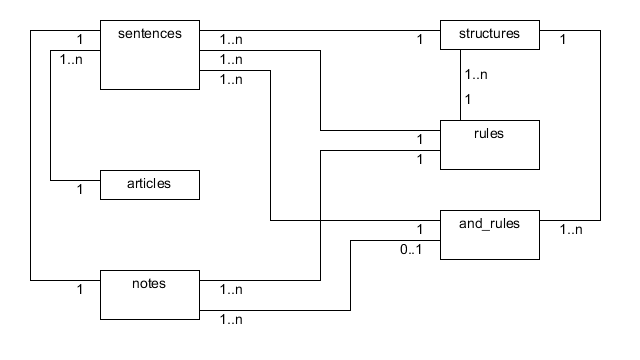
\includegraphics[scale=0.60]{db_schema}\end{center}
	\caption[Databázový model]{Databázový model}\label{fig:db_schema}
\end{figure}

%
% Kolekcia texts
%
\ifthenelse {\boolean{bachelor}}
{
	%\subsection{Subsection}
	\subsubsection{Kolekcia articles}
}
{
	%\section{Subsection}
	\subsection{Kolekcia articles}
}
\label{subsubsection:collection_articles}
V kolekcií \textit{articles} sa ukladajú spracovávané texty. 

Kolekcia obsahuje textové pole \textit{text} na uloženie textu v pôvodnom tvare. Model kolekcie \textit{articles} je zobrazený na obrázku~\fullref{fig:articles_collection_model}.

\begin{figure}[H]
	\begin{center}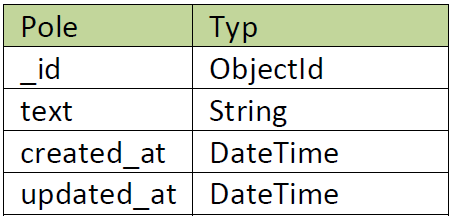
\includegraphics[scale=0.60]{articles_model}\end{center}
	\caption[Model kolekcie articles]{Model kolekcie articles}\label{fig:articles_collection_model}
\end{figure}

%
% Kolekcia notes
%
\ifthenelse {\boolean{bachelor}}
{
	%\subsection{Subsection}
	\subsubsection{Kolekcia notes}
}
{
	%\section{Subsection}
	\subsection{Kolekcia notes}
}
\label{subsubsection:collection_notes}
Kolekcia \textit{notes} uchováva vytvorené poznámky z viet.

Obsahuje textové pole \textit{text} s hodnotou poznámky a dve referencujúce polia. Jedno sa odkazuje do kolekcie \textit{rules} na pravidlo, ktoré bolo použité na vytvorenie poznámky. Druhé referencuje použité and\hyph pravidlo v kolekcií \textit{and\textunderscore rules}. Toto pole môže byť prázdne, ak sa and\hyph pravidlo pri vytváraní poznámky nepoužilo. Na obrázku~\fullref{fig:notes_collection_model} je vyobrazený model kolekcie \textit{notes}.

\begin{figure}[H]
	\begin{center}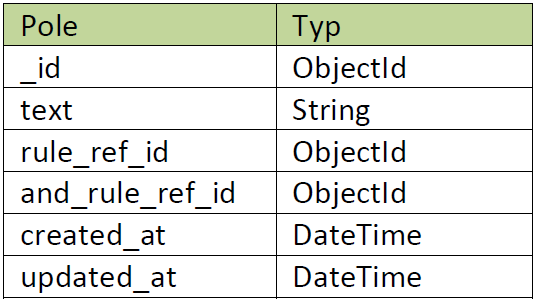
\includegraphics[scale=0.60]{notes_model}\end{center}
	\caption[Model kolekcie notes]{Model kolekcie notes}\label{fig:notes_collection_model}
\end{figure}

%
% Kolekcia sentences
%
\ifthenelse {\boolean{bachelor}}
{
	%\subsection{Subsection}
	\subsubsection{Kolekcia sentences}
}
{
	%\section{Subsection}
	\subsection{Kolekcia sentences}
}
\label{subsubsection:collection_sentences}
V následujúcej kolekcií \textit{sentences} sa ukladajú spracované vety aj s informáciami o článku, pravidlách a poznámke.

Kolekcia sa skladá z textového polia \textit{text} uchovávajúce hodnotu vety a piatich referencujúcich polí \textit{article\textunderscore ref\textunderscore id}, \textit{structure\textunderscore ref\textunderscore id}, \textit{rule\textunderscore id}, \textit{rule\textunderscore ref\textunderscore id}, \textit{and \textunderscore rule\textunderscore ref\textunderscore id} a \textit{note\textunderscore id}. \textit{Article\textunderscore ref\textunderscore id} odkazuje na článok z kolekcie \textit{articles}, ktorého súčasťou je daná veta. Pole \textit{structure\textunderscore ref\textunderscore id} odkazuje do kolekcie \textit{structures}, ktoré reprezentuje štruktúru vety. Nasledujúce polia \textit{rule\textunderscore ref\textunderscore id} a \textit{and\textunderscore rule\textunderscore ref\textunderscore id} odkazujú na použité pravidlo a and\hyph pravidlo pri spracovávaní vety, v tomto poradí. Pole \textit{note\textunderscore ref\textunderscore id} odkazuje na poznámku z kolekcie \textit{notes}, ktorá bola vytvorená z vety.

Model tejto kolekcie je načrtnutý na obrázku~\fullref{fig:sentences_collection_model}.

\begin{figure}[H]
	\begin{center}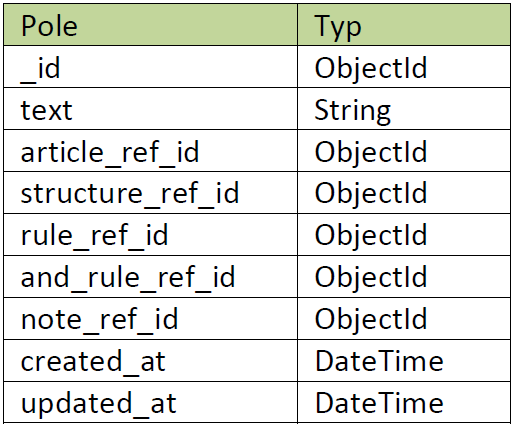
\includegraphics[scale=0.60]{sentences_model}\end{center}
	\caption[Model kolekcie sentences]{Model kolekcie sentences}\label{fig:sentences_collection_model}
\end{figure}

%
% Kolekcia structures
%
\ifthenelse {\boolean{bachelor}}
{
	%\subsection{Subsection}
	\subsubsection{Kolekcia structures}
}
{
	%\section{Subsection}
	\subsection{Kolekcia structures}
}
\label{subsubsection:collection_structures}
V kolekcií \textit{structures} sú uložené štruktúry viet a pravidiel. Štruktúra je zložená hlavne zo závislostí, tokenov, názvoslovných značiek, indexov a iné.

Kolekcia sa skladá z jedného pola \textit{structure\textunderscore data}. Toto pole je zoznam dokumentov, obsahujúcich vyššie spomenuté údaje. Dokument v tomto zozname obsahuje textové pole \textit{relation\textunderscore name} s názvom vzťahu závislosti a zoznam dokumentov závislostí \textit{dependencies} s týmto názvom vzťahu. Dokument v zozname \textit{dependencies} sa skladá z polí \textit{governor} a \textit{dependent} typu dokument, celočíselného pola \textit{position} uchovávajúceho pozíciu závislosti vo vete alebo poznámke, \textit{comparison\textunderscore type}, ktoré je celočíselnou reprezentáciou typu porovnania a poľa \textit{token\textunderscore type}, ktoré je taktiež celočíselnou reprezentáciou typu tokenu. Dokumenty polí \textit{governor} a \textit{depdendent} obsahujú údaje o prislúchajúcich tokenoch závislosti. V textovom poli \textit{POS} sa ukladá značka slovného druhu, pole \textit{index} uchováva index tokenu vo vete, \textit{ner} je textové pole reprezentujúce názvoslovnú entitu tokenu a v poli \textit{lemma} je textová reprezentácia lemy tokenu.

Celý model kolekcie je zobrazený na obrázku~\fullref{fig:structures_collection_model}.

\begin{figure}[H]
	\begin{center}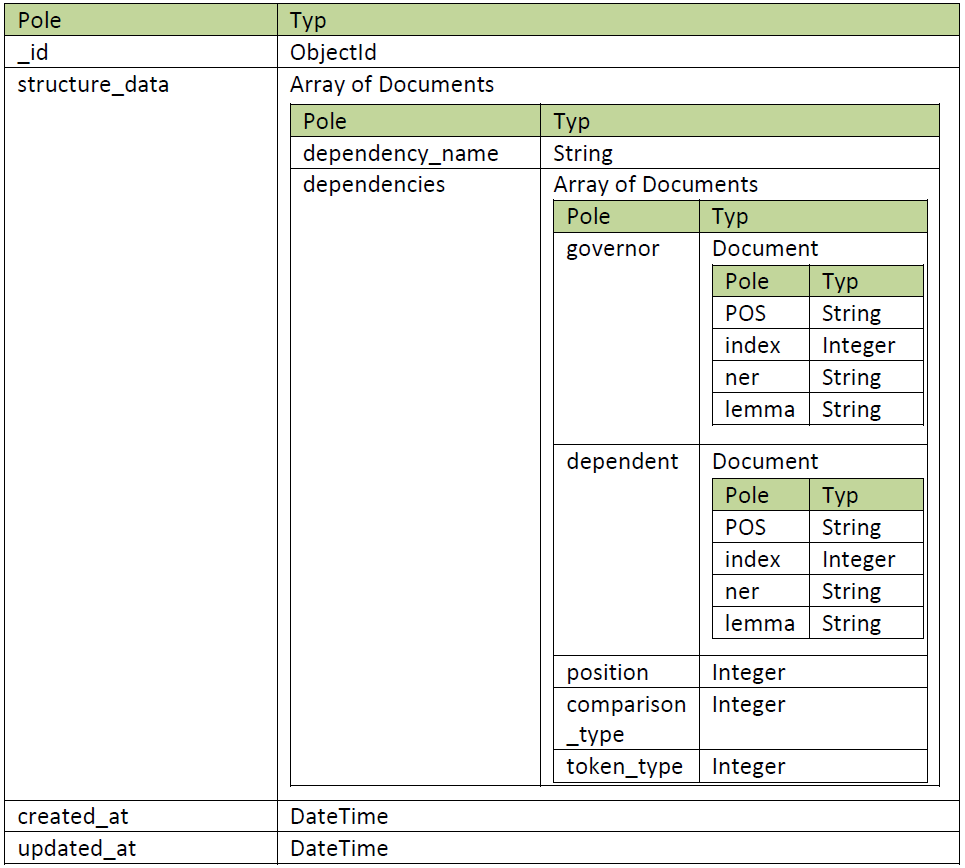
\includegraphics[scale=0.53]{structure_model}\end{center}
	\caption[Model kolekcie structures]{Model kolekcie structures}\label{fig:structures_collection_model}
\end{figure}

%
% Kolekcia rules
%
\ifthenelse {\boolean{bachelor}}
{
	%\subsection{Subsection}
	\subsubsection{Kolekcia rules}
}
{
	%\section{Subsection}
	\subsection{Kolekcia rules}
}
\label{subsubsection:collection_rules}
\textit{Rules} je kolekcia, do ktorej sa ukladajú pravidla na vytvorenie poznámok z viet. Vďaka databázovému modelu na obrázku~\fullref{fig:db_schema} a prepojeniam medzi kolekciami je táto kolekcia minimalistická.

Skladá sa z dvoch polí. Pole \textit{sentence\textunderscore terminators} je zoznam čísel, ktoré reprezentujú konce viet v poznámke. Referencujúce pole \textit{structure\textunderscore ref\textunderscore id} odkazuje do kolekcie \textit{structures} na štruktúru, ktorou sa má prípadná veta spracovať. Model kolekcie \textit{rules} je vyjadrený obrázkom~\fullref{fig:rules_collection_model}.

Pole \textit{sentence\textunderscore terminators} zväčša obsahuje jeden záznam. Napríklad pri vete \textit{,,The president of the Slovak Republic is andrej Kiska.''} a poznámke z tejto vety v tvare \textit{,,President is Kiska.''} bude obsahovať jeden záznam: 3. Číslo 3 preto, lebo koniec vety, v tomto prípade bodka, sa nachádza na tretej pozícií spomedzi tokenov vo vete. Číslovanie pozícií začína  m nula. V prípade ak veta je súvetie, zložené z viacerých jednoduchých viet, môže pole \textit{sentence\textunderscore terminators} obsahovať viacero záznamov, ak napríklad chceme z každej jednoduchej vety súvetia získať zjednodušenú vetu a vytvoriť tak zloženú poznámku, skladajúcu sa zo zjednodušených viet.

\begin{figure}[H]
	\begin{center}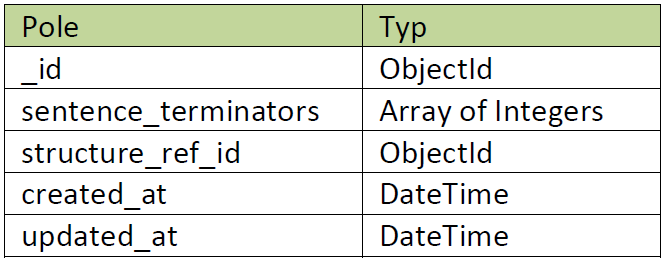
\includegraphics[scale=0.60]{rules_model}\end{center}
	\caption[Model kolekcie rules]{Model kolekcie rules}\label{fig:rules_collection_model}
\end{figure}

%
% Kolekcia and_rules
%
\ifthenelse {\boolean{bachelor}}
{
	%\subsection{Subsection}
	\subsubsection{Kolekcia and rules}
}
{
	%\section{Subsection}
	\subsection{Kolekcia and rules}
}
\label{subsubsection:collection_and_rules}
Posledná kolekcia uchováva pravidlá pre spracovanie vety a vytvorenie viacnásobnej poznámky z vety. Táto kolekcia je veľmi podobná kolekcií \textit{rules} a obsahuje rovnaké polia doplnené o ďalšie špecifické pole.

Špecifické pole, o ktoré je kolekcia rozšírená oproti kolekcií \textit{rules} je celočíselné pole \textit{set\textunderscore position}. Toto pole uchováva pozíciu množiny v viacnásobnej poznámke. Model kolekcie je vyobrazený na obrázku~\fullref{fig:and_rules_collection_model}.

\begin{figure}[H]
	\begin{center}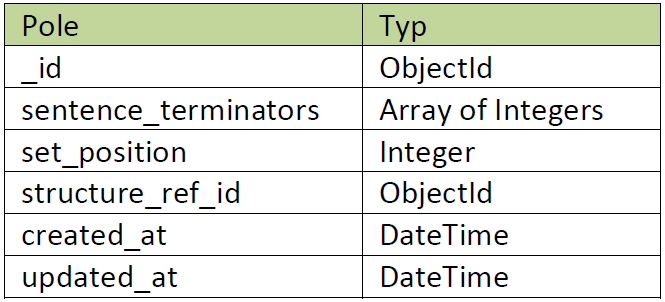
\includegraphics[scale=0.60]{and_rules_model}\end{center}
	\caption[Model kolekcie and rules]{Model kolekcie and rules}\label{fig:and_rules_collection_model}
\end{figure}

%Dáta sú v MongoDB databáze uložené v binárnom JSON formáte. Na ukážke~\fullref{code:collection_rules_data_example} je zobrazená časť uložených údajov o pôvodnej vete. Ukážka celého záznamu pre vetu ,,The president of the Czech Republic is Milos Zeman.'' je priložená v prílohe~\fullref{appendix:db_entry_full_example}.
%\\
%\begin{lstlisting}[language = json, caption={Ukážka dát kolekcie rules}, label = {code:collection_rules_data_example}]
%{  
%	"originalDependencies" : [  
%		{  
%			"dependencyName" : "det",
%			"dependencies" : [  
%				{  
%					"governor" : {  
%						"pos" : "NN",
%						"index" : 2
%					},
%					"dependent" : {  
%						"pos" : "DT",
%						"index" : 1
%					},
%					"position" : 0
%				},
%				{ ... }
%			]
%		}
%	]
%}
%\end{lstlisting}

%
% Kolekcie zhrnutie
%
\ifthenelse {\boolean{bachelor}}
{
	%\subsection{Subsection}
	\subsubsection{Zhrnutie}
}
{
	%\section{Subsection}
	\subsection{Zhrnutie}
}
\label{subsubsection:collections_summary}
Pri návrhu databázového modelu a kolekcií sme vychádzali z princípu jednoduchých kolekcií so zoskupením súvisiacich dát a oddelenia ich od zvyšku. Vďaka využívaniu viacerých, medzi sebou prepojených, kolekcií sme zabezpečili neduplikovanie dát, jednoduché vyhľadanie napríklad viet ku článku a iné. Okrem toho nám tento model umožňuje ďalšiu funkcionalitu, ako napríklad aplikovanie jedného pravidla na viacero viet so zhodnou štruktúrou. Oddelenie dát do samostatných štruktúr nám uľahčuje aj prípadne neskoršie rozšírenie databázového modelu alebo zmenu konkrétnych štruktúr. Taktiež uľahčuje prípadné klastrovanie databázy, ak by bolo nutné, keďže každá kolekcia by mohla byť na samostatnom serveri.


%
% Manažment dát
%
\ifthenelse {\boolean{bachelor}}
{
	%\subsection{Subsection}
	\subsection{Manažment dát}
}
{
	%\section{Subsection}
	\section{Manažment dát}
}
\label{subsection:data_management}
Pre vytvorenie poznámky z vety potrebujeme hlavne vetu a pravidlo, ktoré sa na vetu aplikuje. Aby sa vytvorila zodpovedajúca poznámka z vety, je nutné použiť vhodné pravidlo. Ak spracovávame doposiaľ nespracovanú vetu, je potrebné nájsť vhodné pravidlo na základe podobnosti spracovávanej vety so spracovanými vetami. Pri extrakcií informácií z vety dané pravidlom, s cieľom vytvorenia poznámky sa musia vybrať správne informácie. Extrakcia musí fungovať pri udržaní dostatočnej všeobecnosti, aby sa dané pravidlo dalo aplikovať na viacero viet s rovnakou štruktúrou, ale odlišným obsahom.

%
% Vyhľadávanie pravidla
%
\ifthenelse {\boolean{bachelor}}
{
	%\subsection{Subsection}
	\subsubsection{Vyhľadanie pravidla}
}
{
	%\section{Subsection}
	\subsection{Vyhľadanie pravidla}
}

\label{subsubsection:rule_lookup}
Pri spracovávaní vety, pred vytvorením poznámky, aplikovateľné pravidlo musí byť vyhľadané v databáze. Vyhľadá sa v databáze veta, ktorej štruktúra korešponduje so štruktúrou spracovávanej vety. Štruktúry oboch alebo viacerých viet musia obsahovať rovnakú množinu závislostí. To znamená rovnaký počet záznamov a záznamy s rovnakými názvami vzťahov závislostí v \textit{zozname dát štruktúry}.

Podobná alebo zhodná veta je vyhľadaná, ak hlavná podmienka je splnená. Avšak, splnenie tejto podmienky nezaručí vyhľadanie len jednej, najpodobnejšej vety, ale môže vyhľadať viacero viet. V takom prípade sa vypočíta zhoda viet. Po určení zhody sa extrahuje pravidlo vety, s ktorou má spracovávaná veta najväčšiu zhodu.

%
% Výpočet zhody viet
%
\ifthenelse {\boolean{bachelor}}
{
	%\subsection{Subsection}
	\paragraph{Výpočet zhody viet}
}
{
	%\section{Subsection}
	\subsubsection{Výpočet zhody viet}
}
\label{paragraph:sentences_match}

Zhoda viet pozostáva z troch častí:
\begin{my_itemize}
	\myitem štrukturálna zhoda,
	\myitem obsahová zhoda,
	\myitem hodnotová zhoda.
\end{my_itemize}

Štrukturálna zhoda odzrkadľuje percentuálnu zhody dvoch štruktúr. Pri tejto zhode zisťujeme, či štruktúry obsahujú závislosti s nadradenými značkami slovných druhov a ich konkrétny počet. Štrukturálna zhoda znamená, že vety \textit{,,The president of the Slovak Republic is Andrej Kiska.''} a \textit{,,Andrej Kiska is the president of the Slovak Republic.''}, ale aj \textit{,,Miloš Zeman is the president of the Czech Republic.''} majú rovnakú štruktúru, bez ohľadu na hodnoty a pozície slov vo vete, pokiaľ obsahujú také iste závislosti s rovnakými nadradenými značkami slovných druhov. Definícia nadradenej značky slovného druhu je v časti~\nameref{paragraph:superior_pos_tag} na strane~\pageref{paragraph:superior_pos_tag}. Určenie štrukturálnej zhody pozostáva z niekoľkých krokov. Najskôr sa separátne počíta zhoda nadradených značiek slovných druhov nadradeného a podradeného tokenu. Týmito krokmi sa určí, či veta obsahuje ľubovolnú závislosť s rovnakou nadradenou značkou slovného druhu na ľubovolnom tokene. V nasledujúcom kroku sa určí úplná zhoda závislosti s nadradenými značkami slovných druhov, to znamená zistenie, či veta obsahuje ľubovoľnú závislosť s konkrétnymi značkami slovných druhov na nadradenom a zároveň podradenom tokene. V poslednom kroku sa zisťuje zhoda počtu závislostí s rovnakými nadradenými značkami slovných druhov u nadradeného a podradeného tokenu. \\

Obsahová zhoda zodpovedá percentuálnej zhode obsahu dvoch viet. Kontrolujú sa indexy slov, konkrétne značky slovných druhov a názvoslovné entity. Pri obsahovej zhode majú vety \textit{,,The president of the Slovak Republic is Andrej Kiska.''} a \textit{,,The president of the Czech Republic is Miloš Zeman.''} obsahovú zhodu, bez ohľadu na konkrétne slova na pozíciach vo vete, ak obsahujú rovnaké značky slovných druhov a reprezentujú ich zhodné názvoslovné entity. Výpočet obsahovej zhody sa skladá z viacerých krokov. Začína sa výpočtom zhôd značiek slovných druhov podradeného a nadradeného tokenu. Zhody indexov nadradeného a podradeného tokenu su taktiež vypočítané separátne. Tak isto sa vypočítajú zhody aj názvoslovných entít. Tieto prvé kroky určia, či veta obsahuje ľubovolnú závislosť s rovnakou značkou slovného druho alebo indexom a ľubovoľnú závislosť s rovnakou názvoslovnou entitou. V nasledujúcom kroku je určená polovičná zhoda závislostí. Polovičná zhoda závislosti je zhoda značky slovného druhu a indexu nadradeného alebo podradeného tokenu. Polovičná zhoda sa vypočíta rovnako aj pre názvoslovné entity. Nakoniec, v poslednom kroku, počítame počet úplne zhodných závislostí. Úplná zhoda závislosti je zhoda značky slovného druhu a indexu nadradeného, a zároveň podradeného tokenu. Tak isto sa vypočíta úplná zhoda závislostí aj pre názvoslovné entity. \\

Posledná časť zhody, hodnotová zhoda, reprezentuje úplnú zhodu dvoch viet. Veta má hodnotovú zhodu len s totožnou vetou. \\

Každý krok, pri výpočte všetkých časti zhody, má priradené ohodnotenie. Ak je podmienka v kroku vyhodnotená ako správna, ohodnotenie kroku je pripočítané do finálnej hodnoty. Finálna zhoda je percentuálne ohodnotenie zhody. Ohodnotenie krokov odzrkadľuje dôležitosť daného kroku vo výpočte presnej zhody, pričom závisí od počtu závislostí a krokov, tak že finálna zhoda nemôže presiahnuť hodnotu 100\%. Pseudokód~\ref{alg:calculating_match}~\nameref{alg:calculating_match} zobrazuje algoritmus výpočtu zhody, konkrétny príklad je zobrazený na obrázku~\fullref{fig:calculate_match_sentences_example}

\begin{algorithm}[H]
	\floatname{algorithm}{Algoritmus}
	\footnotesize %\small, \footnotesize, \scriptsize, or \tiny
	\begin{algorithmic}[1]

		\Procedure{VypocetZhodyViet}{$spracovávanáVeta, zavislostiPorovnávanejVety$}
		\State $\text{vypočítaj ohodnotenia krokov}$
		\ForAll {$závislosti\text{ } porovnávanej\text{ } vety$}
		\ForAll {$závislosti\text{ } spracovávanej\text{ } vety$}
		\ForAll {$porovnania$}
		\If {$\text{aplikujPorovnanie(}spracovávanáVeta, porovnanie, závislosť\text{)}$}
		\State $\text{ do zhody na type porovnania pripočítaj ohodnotenie kroku}$
		\EndIf
		\EndFor
		\EndFor
		\EndFor
		
		\Return $zhoda$
		\EndProcedure
	\end{algorithmic}
	\caption[Výpočet zhody viet]{Výpočet zhody viet}	
	\label{alg:calculating_match}
\end{algorithm}

\begin{figure}[H]
	\begin{center}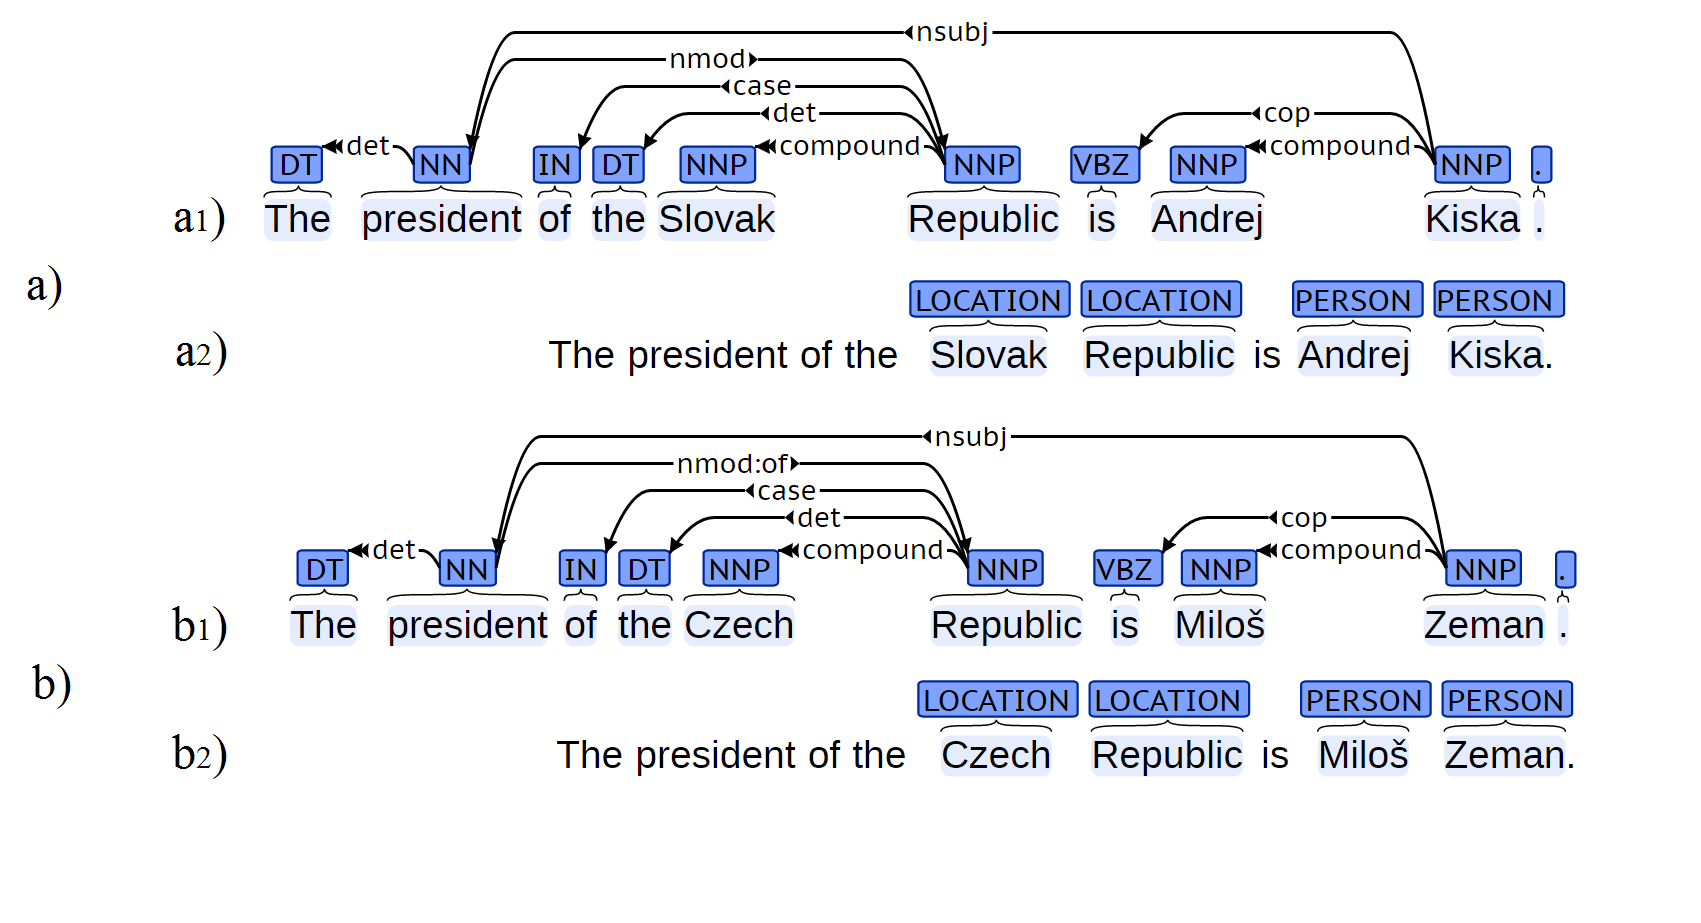
\includegraphics[scale=0.33]{calculate_sentences_match_example}\end{center}
	\caption[Príklad určenia zhody viet]{Príklad určenia zhody viet}\label{fig:calculate_match_sentences_example}
\end{figure}

Predpokladajme situáciu z obrázka~\fullref{fig:calculate_match_sentences_example}. V databáze máme uloženú spracovanú vetu \textit{a} aj s pravidlom pre túto vetu. Spracovávame vetu \textit{b}. Na časti \textit{a1} obrázka~\fullref{fig:calculate_match_sentences_example} sú znázornené závislostí a na časti \textit{a2} názvoslovné entity vety \textit{a}. Na časti \textit{b1} sú znázornené závislostí a na časti \textit{b2} názvoslovné entity vety \textit{b}. V tejto situácií potrebujeme vypočítať zhodu medzi vetami \textit{a} a \textit{b}. 

Pri štrukturálnej časti zhody sa prechádza cez všetky závislosti vety \textit{a}. Prvá závislosť je závislosť so vzťahom \textit{DET} a nadradeným tokenom s nadradenou značkou slovného druhu \textit{NN} a podradeným tokenom s nadradenou značkou slovného druhu \textit{DT}. V prom kroku sa pozrie, či veta \textit{b} obsahuje ľubovoľnú závislosť s podradeným tokenom s nadradenou značkou slovného druhu \textit{DT}. V ďalšom kroku, sa zistí, či veta \textit{b} obsahuje ľubovoľnú závislosť s nadradeným tokenom s nadradenou značkou sloveného druhu \textit{NN}. Môže to byť aj iná závislosť, ako tá z prvého kroku. Pokračuje sa zistením úplnej zhody závislosti. Určí sa , či veta \textbf{b} obsahuje ľubovoľnú závislosť s podradeným tokenom s nadradenou značkou slovného druhu práve \textit{DT} a zároveň s nadradeným tokenom s nadradenou značkou slovného druhu \textit{NN}. Takto sa iteruje cez všetky závislosti vety \textit{a}. Na záver sa určí zhoda počtu závislostí s rovnakou štruktúrou. Napríklad veta \textit{a} obsahuje práve dve závislosti, ktoré majú na podradenom tokene nadradenú značku slového druhu \textit{DT} a na nadradenom tokene nadradenú značku slovného druhu \textit{NN}. Zistí sa, či aj veta \textit{b} obsahuje práve dve takéto závislosti. \\

Prvá závislosť vo vete \textit{b} je so vzťahom \textit{det}, nadradeným tokenom so značkou slovného druhu \textit{NN} a indexom 1 a podradeným tokenom so značkou slovného druhu \textit{DT} a indexom 0. Token slova \textit{Slovak} má názvoslovnú entity typu \textit{LOCATION - lokácia}. Ak slovo nemá vyobrazený typ názvoslovnej entity, znamená to, že má názvoslovnú entity typu \textit{OTHER - ostatné}. V prvok kroku pri určovaní obsahovej časti zhody zisťujeme, či veta \textit{b} obsahuje závislosť so vzťahom \textit{det} a tokenmi so značkou slovného druhu \textit{NN} alebo \textit{DT} a indexmi rovnými 0 alebo 1. Toto je separátny výpočet značiek slovných druhov a indexov. V tomto isto kroku sa tiež pozrie, či veta \textit{b} obsahuje ľubovoľnú závislosť s podradeným tokenon s názvoslovnou entitou typu \textit{ostatné} (názvoslovná entita tokenu \textit{THE} vo vete \textit{a}) a ľubovoľnú závislosť s nadradeným tokenom s názvoslovnou entitou typu \textit{ostatné} (názvoslovná entita tokenu \textit{president} vo vete \textit{a}). V nasledujúcom kroku zisťujeme, či veta \textit{b} obsahuje závislosť so vzťahom \textit{det} a nadradeným alebo podradeným tokenom so značkou slovného druhu \textit{NN} a indexom 1 alebo značkou slovného druhu \textit{DT} a indexom 0. Toto je polovičná zhoda. V poslednom kroku hľadáme vo vete \textit{b} závislosť so vzťahom \textit{det} a nadradeným tokenom práve so značkou slovného druhu \textit{NN} a indexom 1 a zároveň podradeným tokenom práve so značkou slovného druhu \textit{DT} a indexom 0. Zároveň v tomto kroku sa zisťuje, či veta \textit{b} obsahuje závislosť s podradeným tokenom s názvoslovnou entitou typu \textit{ostatné} a zároveň s nadradeným tokenom s názvoslovnou entitou typy \textit{ostatné}. Iterácia pokračuje s nasledujúcou závislosťou, pokým sa nevyhodnotia všetky. \\

Pri určení hodnotovej časti zhody sa porovnajú texty \textit{,,The president of the Slovak Republic is Andrej Kiska.''} a \textit{,,The president of the Czech Republic is Miloš Zeman.''} a určí sa, či su zhodné. \\

Aplikovaním určenia zhody viet medzi vetami \textit{a} a \textit{b} zistíme, že veta \textit{b} má štrukturálnu časť zhody s vetou \textit{a} $100\%$. Tak isto má obsahovú časť zhody rovnú $100\%$. Hodnotová časť zhody je $0\%$.

%
% Nadradená značka slovného druhu
%
\ifthenelse {\boolean{bachelor}}
{
	%\subsection{Subsection}
	\paragraph{Nadradená značka slovného druhu}
}
{
	%\section{Subsection}
	\subsubsection{Nadradená značka slovného druhu}
}
\label{paragraph:superior_pos_tag}

Pod nadradenou značkou slovného druhu sa chápe značka slovného druhu zoskupujúca množinu značiek slovných druhov, do ktorej značka slovného druhu patrí. 

Napríklad značka slovného druhu VBD (Verb, past tense - sloveso v minulom čase) patrí medzi skupinu značiek slovných druhov slovies \textit{\{VB, VBD, VBG, VBN, VBP, VBZ\}}. Z toho vyplýva, že nadradená značka slovného druhu \textit{VBD} je VB (Verb - sloveso).

%
% Aplikovanie pravidla
%
\ifthenelse {\boolean{bachelor}}
{
	%\subsection{Subsection}
	\subsubsection{Aplikovanie pravidla}
}
{
	%\section{Subsection}
	\subsection{Aplikovanie pravidla}
}
\label{subsubsection:rule_application}

Procesom vyhľadania pravidla (viď.~\fullref{subsubsection:rule_lookup}) sme získali pravidlo na spracovanie vety. Aplikáciou pravidla na vetu vytvoríme poznámku.

Proces aplikovania pravidla na vetu s cieľom vytvorenia poznámky má viacero krokov. Pre všetky závislosti zo \textit{zoznamu dát štruktúry} pravidla, príslušná závislosť je vyhľadaná v spracovávanej vete. Pri vyhľadávaní príslušnej závislosti sa závislosti neporovnávajú, okrem iného, na základe značiek slovných druhov svojich tokenov, ale podľa nadradených značiek slovných druhov (viď.~\nameref{paragraph:superior_pos_tag} na strane~\pageref{paragraph:superior_pos_tag}) svojich tokenov. Tento spôsob vyhľadávania nám umožňuje [BLA BLA, blizie opisane v BLA BLA]. Avšak, môže to spôsobiť vyhľadanie viac ako jednej príslušnej závislosti. Preto musí byť vypočítaná zhoda závislostí (viď.~\nameref{paragraph:dependency_match} na strane \pageref{paragraph:dependency_match}). Po vypočítaní zhody závislostí a získanie závislosti s najväčšou zhodou, slovo korešpondujúce s tokenom, ktorý sa ma z danej závislosti vybrať, sa pridá do poznámky na pozíciu pozície závislosti. Po spracovaní všetkých závislostí, posledné minoritné úpravy sú vykonané nad poznámkou, ako rozdelenie na viacero viet, ak tak určovalo pravidlo, kapitalizácia prvých písmen viet poznámky a iné. Pseudokód aplikovania pravidla na vetu s cieľom vytvoriť poznámku je zobrazený na algoritme~\ref{alg:applying_rule}.

\begin{algorithm}
	\floatname{algorithm}{Algoritmus}
	\caption[Aplikovanie pravidla]{Aplikovanie pravidla}\label{alg:applying_rule}
	\begin{algorithmic}[1]
		\Procedure{ApplyRule}{$sentence, rule$}
		\State $note \gets \text{new Note}$
		\ForAll {$ruleDependencies$}
		\State $dependency \gets \text{findDependency(} sentence \text{, } ruleDependency \text{)}$
		\If {$\text{isFound(}dependency\text{)}$}
		\State $\text{add(} note \text{, getDependent(} dependency \text{))}$
		\If {$\text{isNominalSubject(relation(}dependency \text{))}$}
		\State $\text{add(} note \text{, getGovernor(} dependency \text{))}$
		\EndIf
		\EndIf
		\EndFor
		
		\State $\text{splitToSentences(} note \text{, sentencesEnds(} rule \text{))}$	
		
		\Return $note$
		\EndProcedure
	\end{algorithmic}
\end{algorithm}

Pre vetu \textit{,,The president of the Slovak republic is Andrej Kiska.''} nám nástroj Stanford CoreNLP poskytne závislostí vyobrazené na obrázku~\fullref{fig:example_sentence_andrej_kiska}. Ak na túto vetu aplikujeme pravidlo so štruktúrou v tvare zobrazenej na obrázku~\fullref{fig:apply_rule_example_rule}, výsledná poznámka bude \textit{,,President is Kiska.''}. 

Aplikovanie pravidla prebieha nasledovným spôsobom. Prechádzajú sa všetky závislosti v štruktúre pravidla. Prvá závislosť v štruktúre pravidla je závislosť so vzťahom \textit{nsubj} na pozícií jedna a podradeným korešpondujúcim tokenom. Má podradený token so značkou slovného druhu \textit{NN}, typom názvoslovnej entity \textit{OTHER - ostatné}, lemou \textit{President} a indexom dva. Nadradený token má značku slovného druhu \textit{NNP}, názvoslovnú entitu \textit{PERSON - osoba}, lemu \textit{Kiska} a index deväť. Takáto závislosť sa vyhľadá v štruktúre vety medzi závislosťami na obrázku~\fullref{fig:example_sentence_andrej_kiska}. Ak pre danú závislosť vyhovuje viacero závislostí, pomocou výpočtu zhody závislostí vyberieme tú s najväčšou zhodou. V tomto prípade vidíme, že vyhovujúca závislosť je len jedna a to prvá závislosť \textit{nsubj} medzi slovom na druhej pozícií \textit{president} a posledným slovom, na deviatej pozícií \textit{Kiska}. Z tejto závislosti sa zoberie podradený token, keďže tak určuje pravidlo v stĺpci \textit{typ tokenu}. Slovo \textit{president} sa pridá do poznámky na pozíciu jedna. Rovnakým spôsobom sa prechádzajú a spracujú všetky závislosti v štruktúre pravidla a podľa nich sa extrahuje slovo z vety a pridá do poznámky.

\begin{figure}[H]
	\begin{center}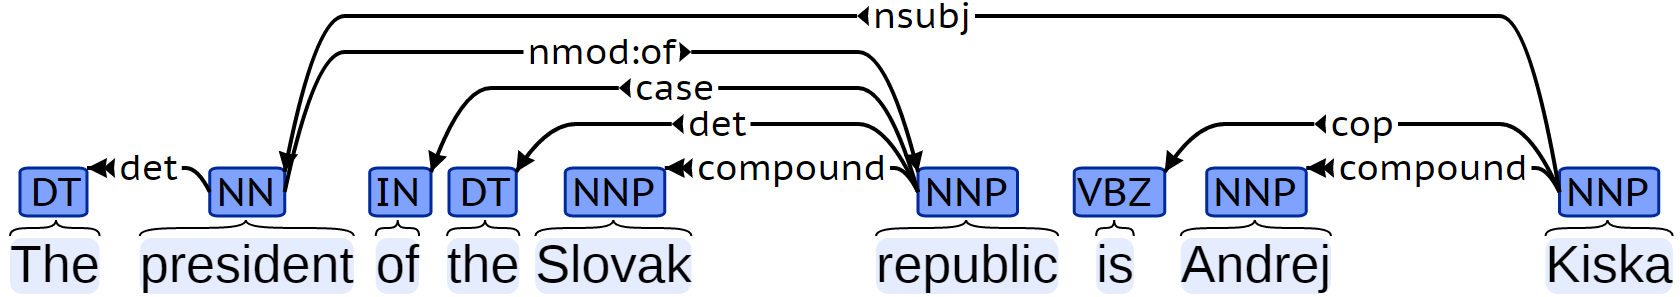
\includegraphics[scale=0.32]{example_sentence_andrej_kiska}\end{center}
	\caption[Zásivlostí jednoduchej vety]{Zásivlostí jednoduchej vety}\label{fig:example_sentence_andrej_kiska}
\end{figure}

\begin{figure}[H]
	\begin{center}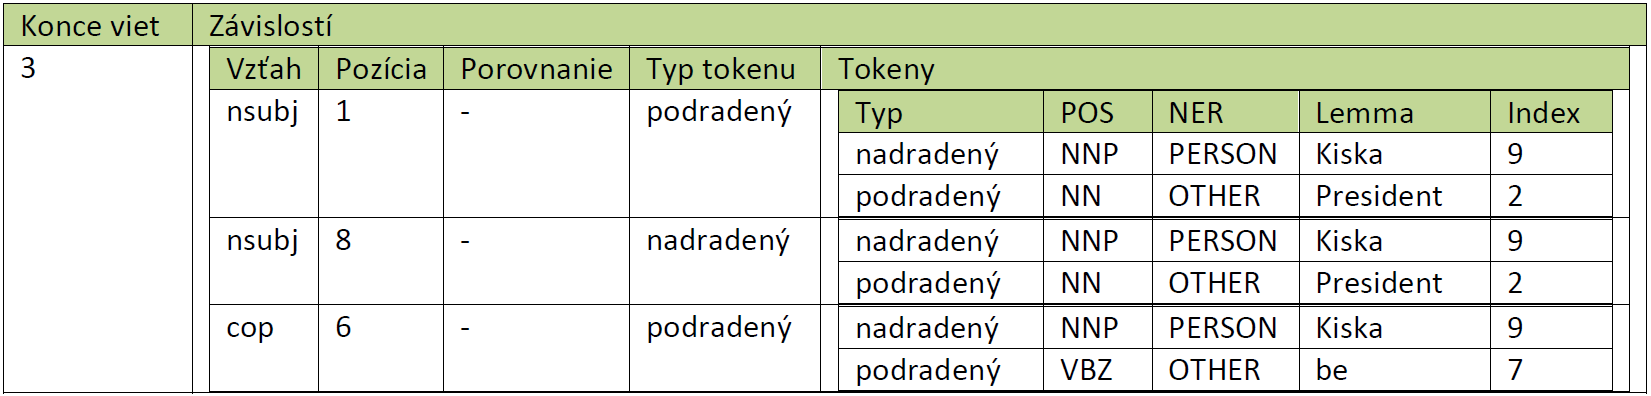
\includegraphics[scale=0.32]{apply_rule_example_rule}\end{center}
	\caption[Príklad štruktúry pravidla]{Príklad štruktúry pravidla}\label{fig:apply_rule_example_rule}
\end{figure}

%
% Výpočet zhody závislostí
%
\ifthenelse {\boolean{bachelor}}
{
	%\subsection{Subsection}
	\paragraph{Výpočet zhody závislostí}
}
{
	%\section{Subsection}
	\subsubsection{Výpočet zhody závislostí}
}
\label{paragraph:dependency_match}

Princíp výpočtu zhody závislostí je veľmi podobný s výpočtom zhody viet zo sekcie~\fullref{subsubsection:rule_lookup}. Porovnávajú sa vždy nadradené aj podradené tokeny. Porovnanie má niekoľko krokov. Začína sa s porovnaním značiek slovných druhov. Pokračuje sa názvoslovnou entitou, indexom, lemou a nakoniec sa porovnáva vzdialenosť pozícií tokenov vo vetách. Každý krok je príslušne ohodnotený a ak porovnanie bolo úspešné, ohodnotenie sa pripočíta k finálnej hodnote reprezentujúcej percentuálnej zhody závislostí.

%
% Vytváranie pravidla
%
\ifthenelse {\boolean{bachelor}}
{
	%\subsection{Subsection}
	\subsubsection{Vytvorenie pravidla}
}
{
	%\section{Subsection}
	\subsection{Vytvorenie pravidla}
}
\label{subsubsection:rule_creation}
Ak nám proces vyhľadania pravidla nevyhľadal žiadne pravidlo, znamená to, že sme doposiaľ nespracovávali takú istú alebo podobnú vetu. V tomto prípade sú použité statické pravidlá na spracovanie vety. Výstupom bude zjednodušená veta - poznámka.

Vytvorí sa záznam o pôvodnej vete, ktorý okrem iného obsahuje \textit{zoznam dát o pôvodnej vete}, ktorý sa vyskladá zo závislostí vety. Následne sa vytvorí záznam o pravidle, ktorý okrem iného obsahuje \textit{zoznam dát o poznámke}, vyskladaný zo závislosti poznámky. Nakoniec sa tieto dva záznamy prepoja a tým sa vytvorí nové pravidlo na spracovanie takej istej alebo podobnej vety, akú sme práve spracovali.

%Na obrázku~\fullref{fig:rule_creation} je znázornený proces nevyhľadania pravidla, použitia parsera s následným uložením nového pravidla.

%\begin{figure}[H]
%	\begin{center}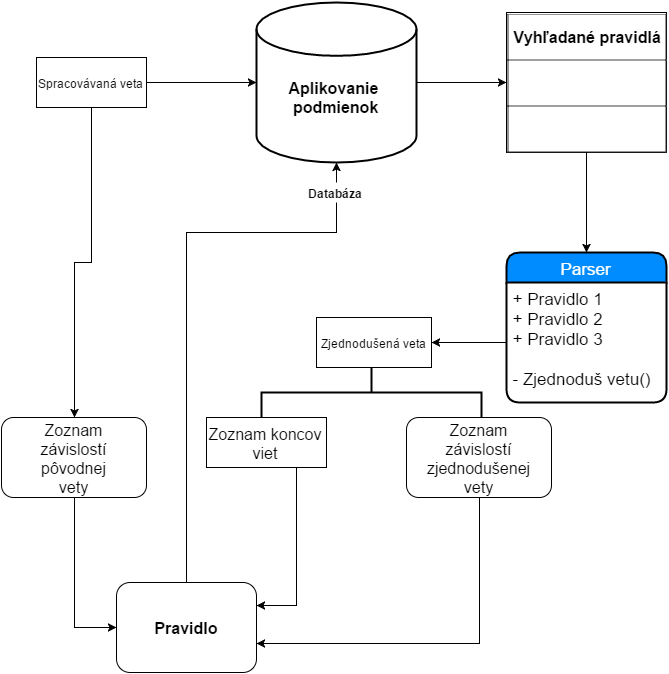
\includegraphics[scale=0.5]{rule_creation}\end{center}
%	\caption[Vytvorenie pravidla]{Vytvorenie pravidla}\label{fig:rule_creation}
%\end{figure}

%%
%% test
%%
\newpage
\ifthenelse {\boolean{bachelor}}
{
	%\section{Results}
	\section{Experimenty}
}
{
	%\chapter{Results}
	\chapter{Experimenty}
}
\label{experiments}
Na systéme boli vykonané tri experimenty. V prvom experimente bol systém porovnaný so systémom na sumarizáciu textu. Druhý experiment overoval použitie pravidiel na základe štruktúry viet. Posledný bol používateľský experiment, počas ktorého bol náš systém testovaný reálnymi používateľmi.

\subsection{Porovnanie systému}
\label{experiments:first_experiment}
V prvom experimente sme náš systém použili na spracovanie troch článkov z wikipádie~\footnote{www.simple.wikipedia.org}. Výsledky sme porovnali s Autosummarizer~\footnote{www.autosummarizer.com}, systémom zameraným na sumarizáciu textu, využívajúci extrakčnú sumarizáciu. Články obsahovali spolu 27 viet a 294 slov.

\subsubsection{Výsledky}
\label{experiments:first_experiment:results}
Porovnali sme počty viet a slov na výstupe systémov. Počty sú na~\imgref{experiments:first_experiment:results:fig:output}. V časti \textit{a} je zobrazený počet viet a v časti \textit{b} je počet slov. V druhej časti porovnania sme sa zamerali na prístup systémov k spracovaniu viet a slov. Na~\imgref{experiments:first_experiment:results:fig:processing} v časti \textit{a} je zobrazený počet viet, ktoré systémy nespracovali a v časti \textit{b} je priemerný počet eliminovaných irelevantných slov vo výslednej vete. 

\begin{figure}[H]%
	\centering
	\subfloat[Počet viet na výstupe]{{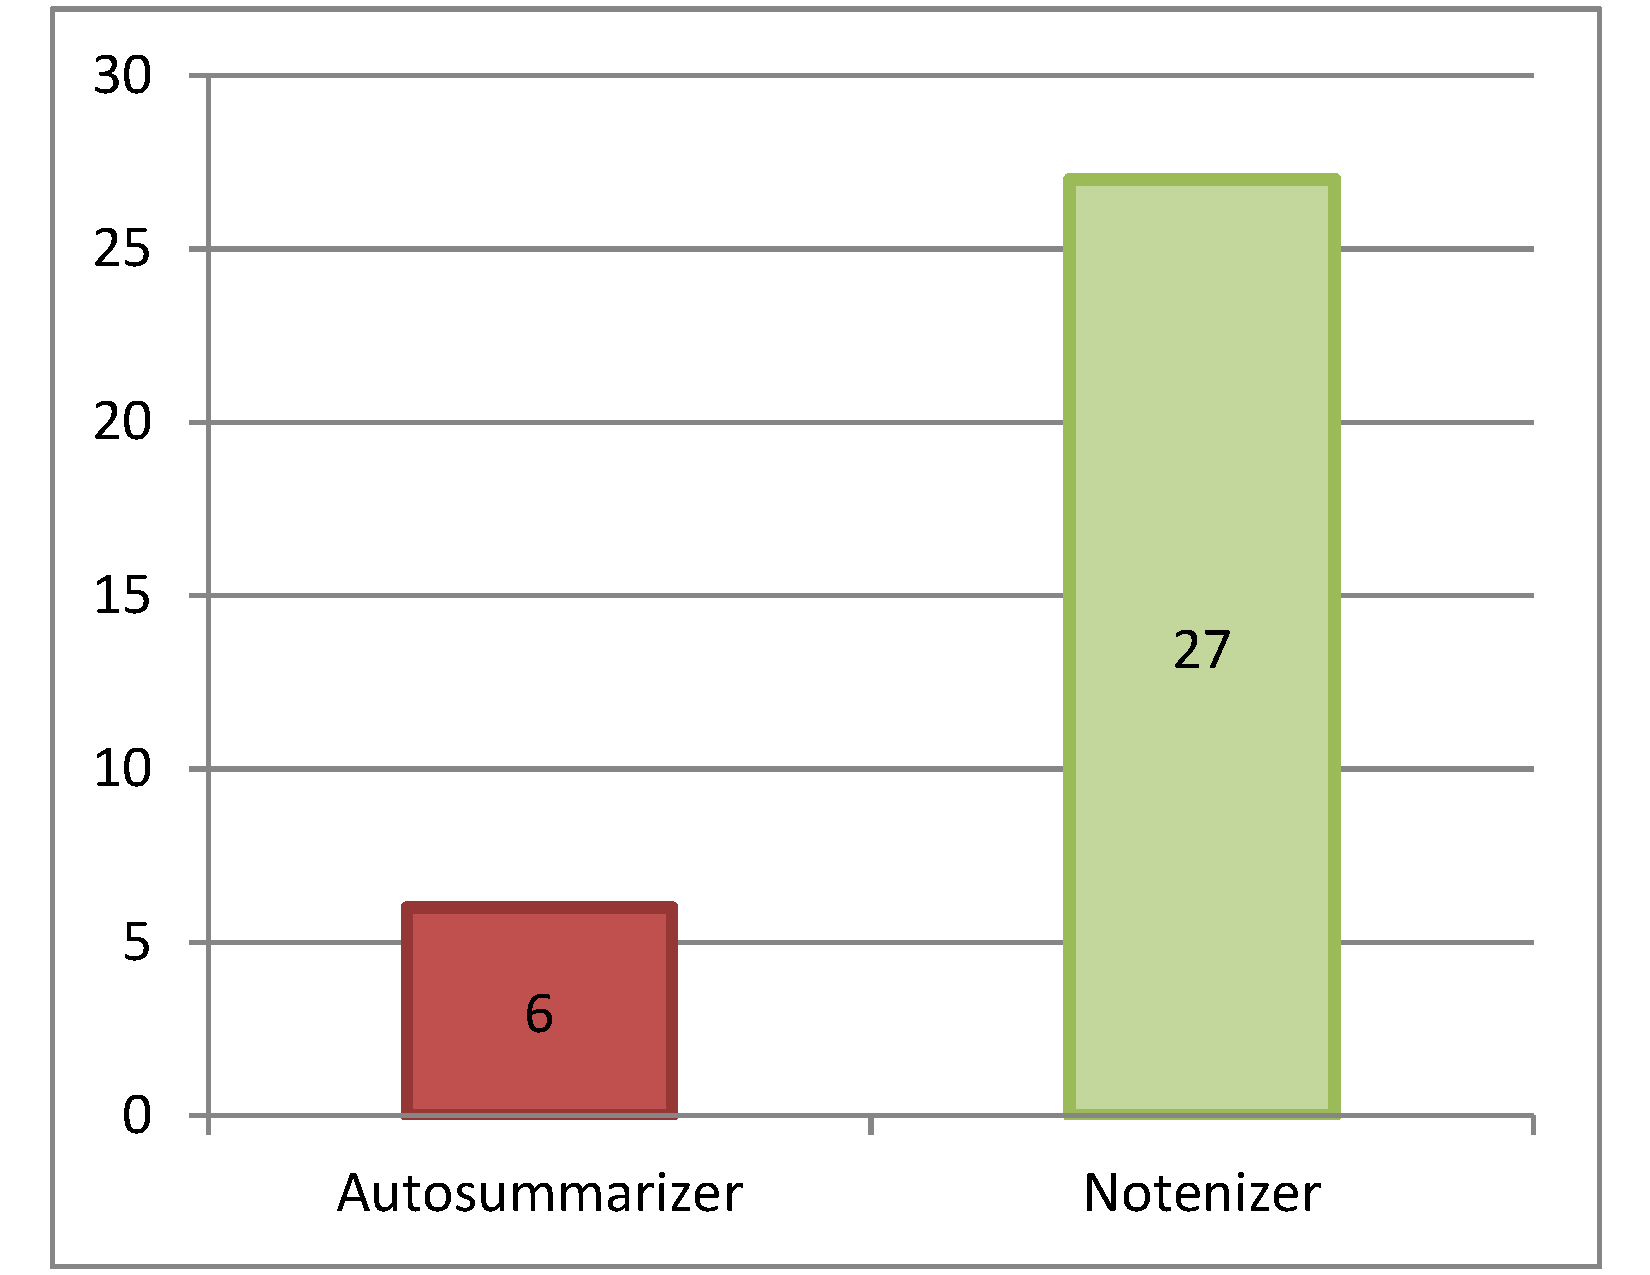
\includegraphics[scale=0.22]{exp_exp_sentences_output} }}%
	\qquad
	\subfloat[Počet slov na výstupe]{{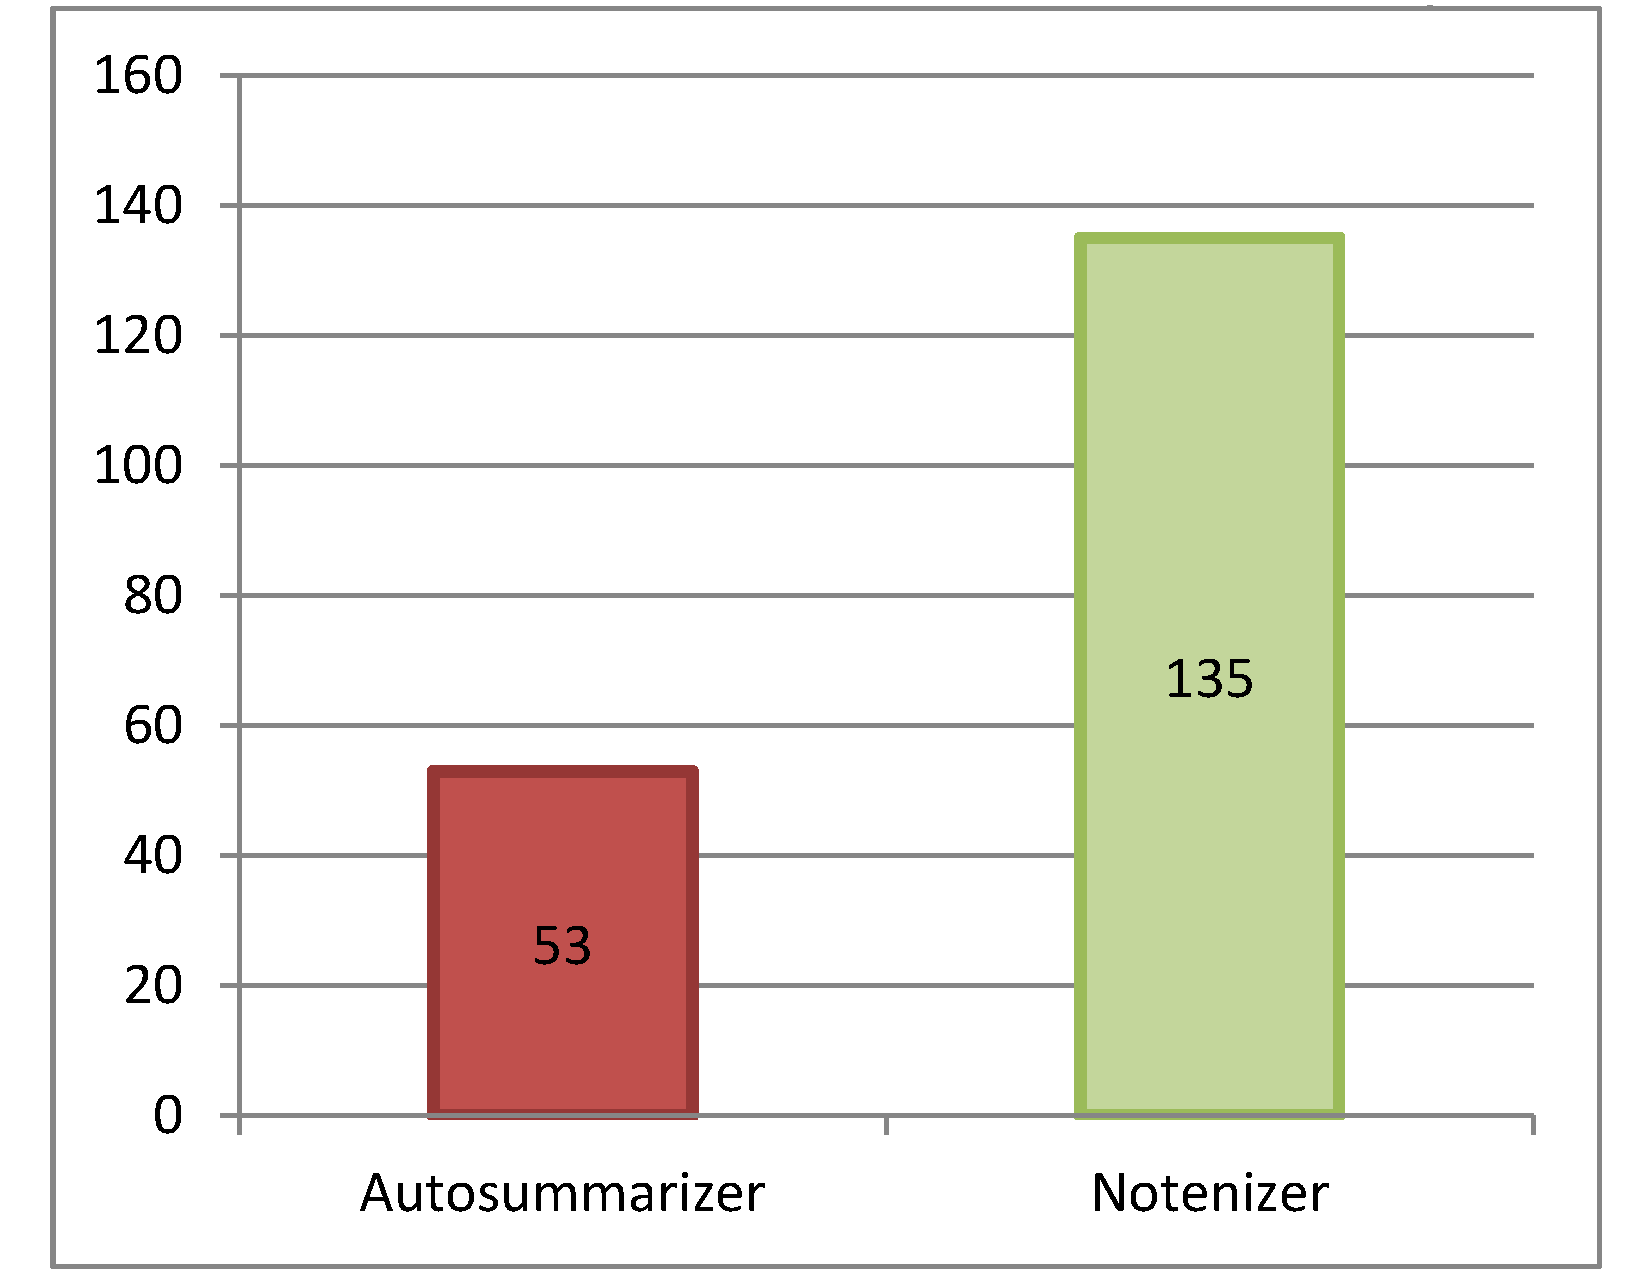
\includegraphics[scale=0.22]{exp_exp_words_output} }}%
	\caption{Výstupy porovnaných systémov}%
	\label{experiments:first_experiment:results:fig:output}%
\end{figure}

\begin{figure}[H]%
	\centering
	\subfloat[Počet nespracovaných viet]{{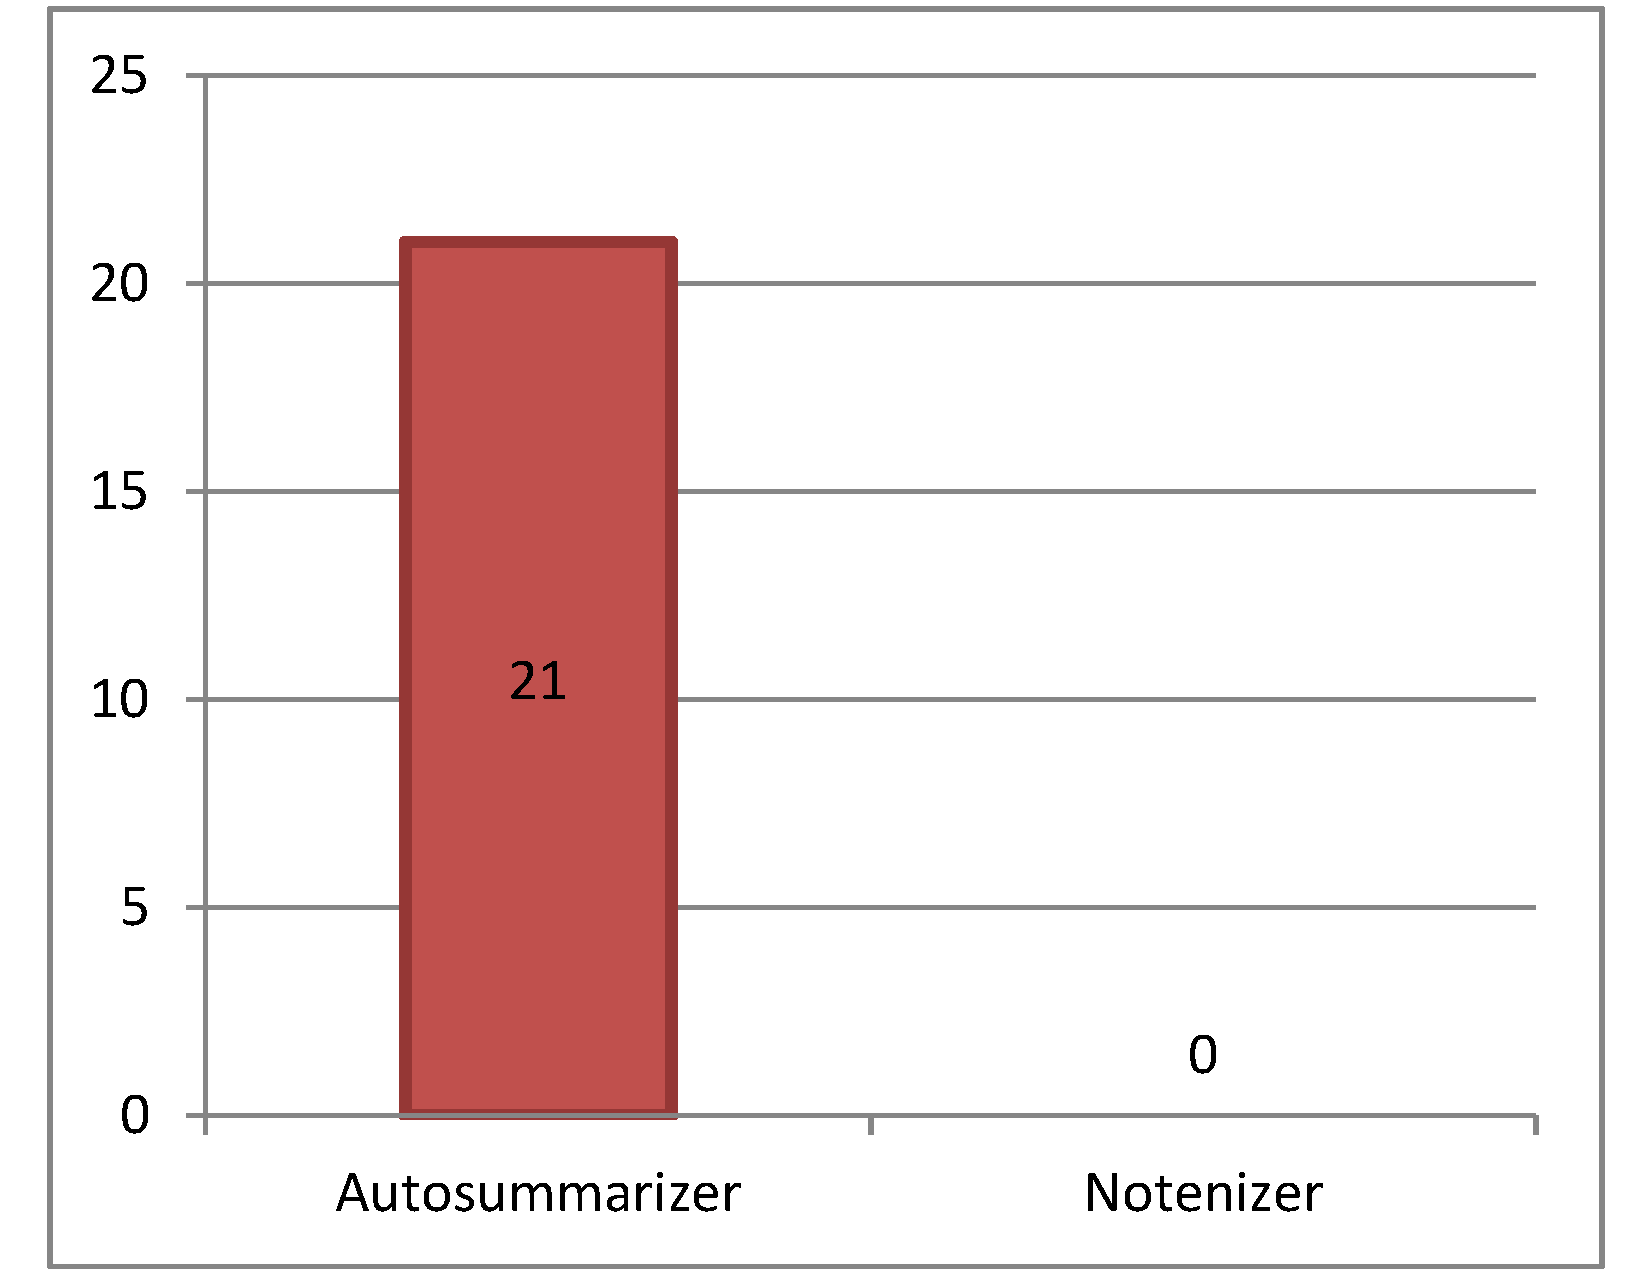
\includegraphics[scale=0.22]{exp_exp_sentences_not_processed} }}%
	\qquad
	\subfloat[Priemerný počet eliminovaných irelevantných slov vo výslednej vete]{{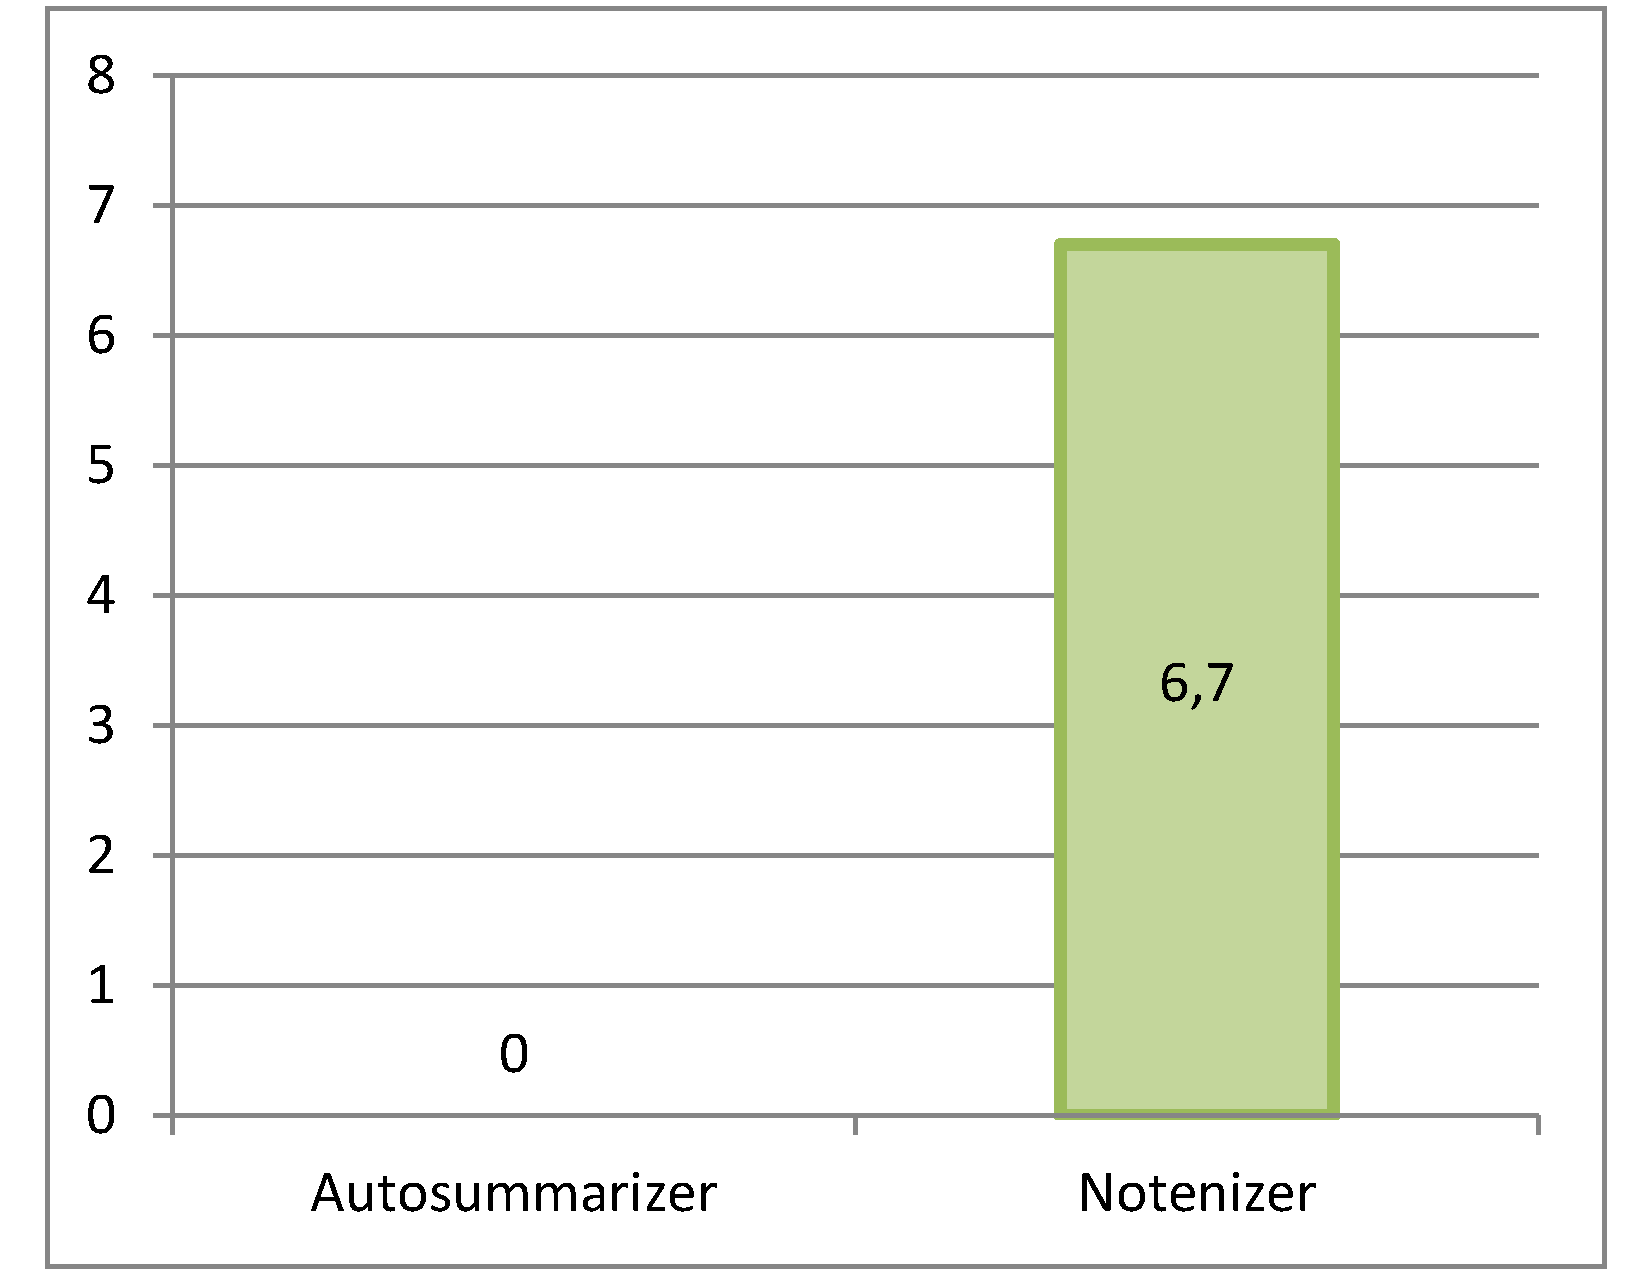
\includegraphics[scale=0.22]{exp_exp_irrelevant_words_eliminated_avg} }}%
	\caption{Spracovanie informácií porovnanými systémami}%
	\label{experiments:first_experiment:results:fig:processing}%
\end{figure}

\subsubsection{Vyhodnotenie porovnania}
Autosummarizer systém dosahoval lepšie výsledky v menšom počte viet a slov na výstupe, ale kvôli tomu vynechal veľa relevantných informácií. Náš systém na výstupe zobrazoval väčšie množstvo slov a viet, avšak spracoval všetky vety a eliminoval z nich irelevantné informácie, slová.

\subsection{Použitie pravidiel}
Otestovali sme aplikovateľnosť pravidiel závislých od štruktúry vety. Pri spracovaní $340$ viet z tridsiatich článkov bolo potrebné vytvoriť a použiť $263$ pravidiel. Z toho vyplýva, že pri $77$ vetách bolo aplikované pravidlo na základe štruktúry vety a nebolo potrebné vytvárať nové. To predstavuje približne $22,65\%$ všetkých viet, čím sa nám podarilo práve takéto množstvo pravidiel ušetriť.

\subsection{Používateľský experiment}
\label{experiments:main_experiment}
Na používateľskom experiment sa zúčastnilo pätnásť študentov, ktorí v systéme spracovali článok a získali z neho poznámky. Množina článkov experimentu pozostávala z článkov z wikipédie\footnote{www.simple.wikipedia.org} o štátoch z Európy. Účastník experimentu si zvolil článok, ktorý sa následne spracoval. Experiment sa skladal z dvoch častí. V prvej časti sa článok vybraný účastníkom spracoval nad databázou, ktorá obsahovala počet pravidiel z piatich vopred spracovaných článkov. V druhej časti sa ten istý článok spracoval nad databázou s tridsiatimi vopred spracovanými článkami. Účastník v oboch častiach experimentu vytvorené poznámky z viet článku ohodnotil, prípadne upravil. Všetci účastníci testovali systém nad databázami s rovnakými dátami. Počas experimentu bolo spracovaných pätnásť článkov s $236$ vetami.

\subsubsection{Výsledky}
\label{experiments:main_experiment:results}
Na~\imgref{experiments:user_experiment:results:fig:exp_general_comparison} sú zobrazené pomery správnych a nesprávnych vytvorených poznámok. Na časti \textit{a} tohoto obrázka vidno pomer pri spracovaní článku v prvej časti experimentu a v časti \textit{b} je pomer z druhej časti experimentu.

\begin{figure}[H]%
	\centering
	\subfloat[Všeobecné výsledky prvej časti]{{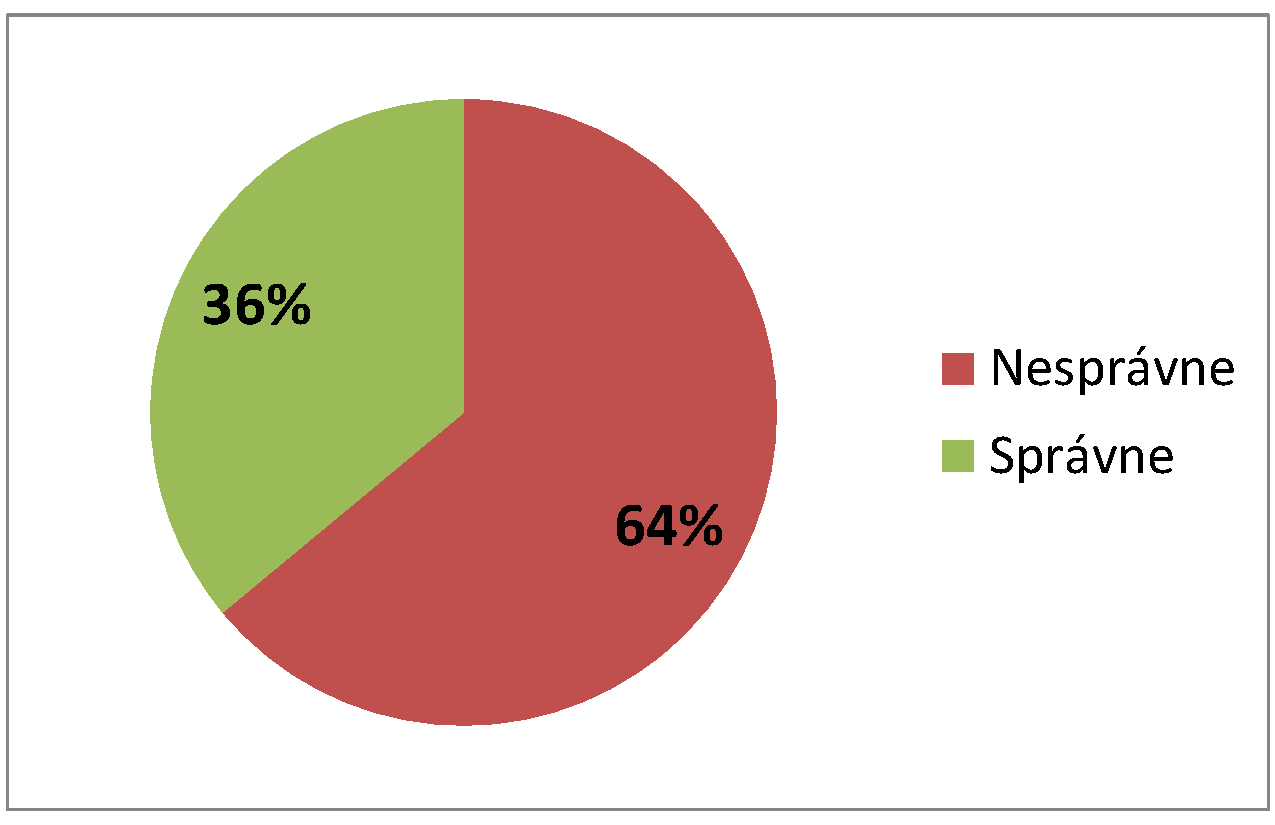
\includegraphics[scale=0.29]{exp_first_general} }}%
	\qquad
	\subfloat[Všeobecné výsledky druhej časti]{{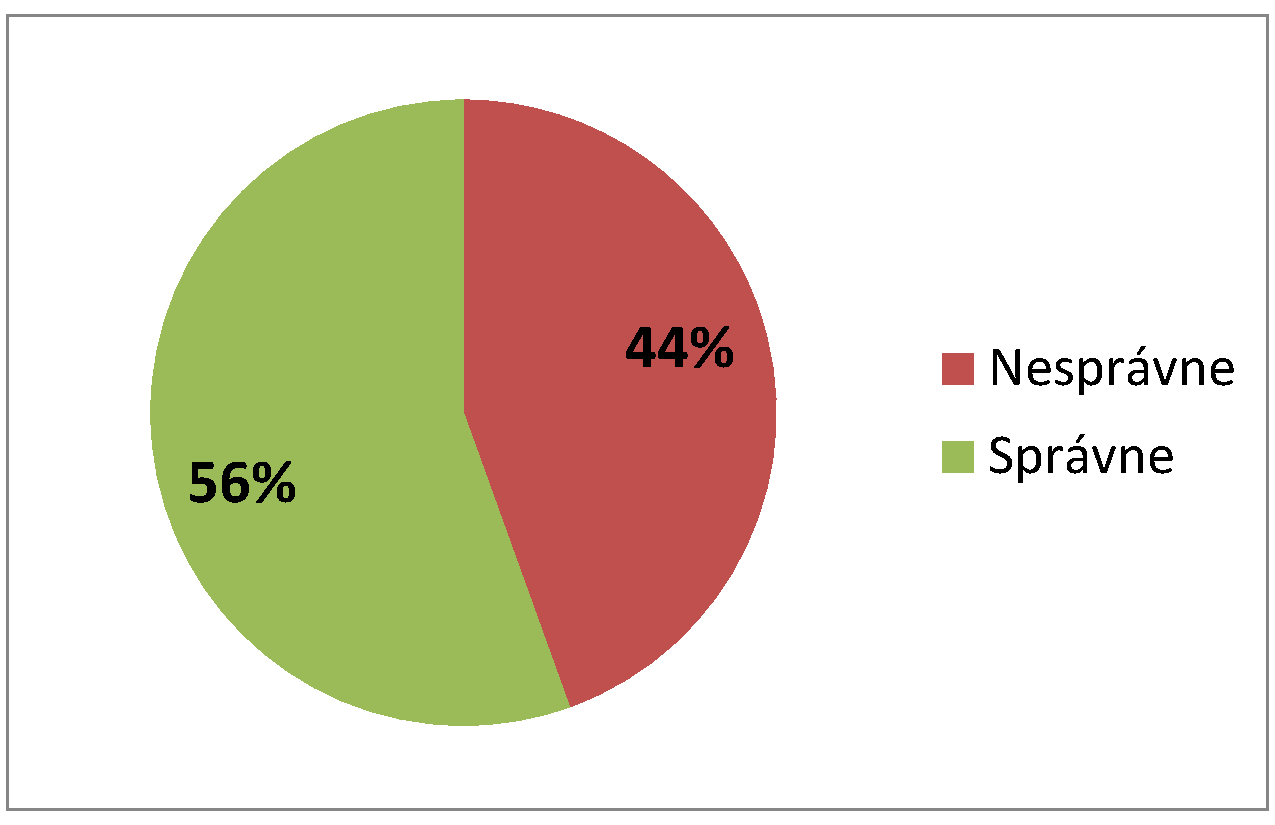
\includegraphics[scale=0.29]{exp_second_general} }}%
	\caption{Porovnanie všeobecných výsledkov oboch časti experimentu}%
	\label{experiments:user_experiment:results:fig:exp_general_comparison}%
\end{figure}

Správne aj nesprávne poznámky boli podľa hodnotení účastníkov kategorizované do štrnástich kategórií. Najpočetnejšie z nich sú pre nesprávne poznámky \textit{zlé spracované, chýba podstatná informácia, chýba mala časť informácie} a pre správne poznámky sú to \textit{správne, OK - zlý slovosled, OK - subjektívne}.

\textit{Zle spracované} znamená, že systém zle spracoval vetu a vytvorená poznámka neobsahovala takmer žiadnu informáciu a nedávala zmysel. V kategórií \textit{chýba podstatná informácia} sú zaradené poznámky, ktoré boli korektne vytvorené, avšak chýbala v nich podstatná informácia z vety potrebná na jej pochopenie. V poznámkach, ktoré obsahovali veľkú časť podstatnej informácie, prípadne celú podstatnú informáciu, ale chýbala v nej malá časť informácie z pôvodnej vety potrebná na to, aby sa dala považovať za správnu poznámku, boli zaradené do kategórie \textit{chýba mala časť informácie}. Do kategórie \textit{správne} boli zaradené poznámky, ktoré boli správne vytvorené. Kategória \textit{OK - zlý slovosled} obsahuje poznámky, ktoré obsahovali celú podstatnú informáciu z vety, ale slovosled vety bol zlý. Poznámky, ktoré boli označené za správne, ale účastník sa vyjadril, že si vie predstaviť, že pre niekoho by daná poznámka nemusela byť správna, boli zaradené do kategórie \textit{OK - subjektívne}.

Na~\imgref{experiments:user_experiment:results:fig:exp_detailed_comparison_first} a~\imgref{experiments:user_experiment:results:fig:exp_detailed_comparison_second} sú zobrazené percentuálne zastúpenia kategórií pri prvej a druhej časti experimentu, v tomto poradí.

\begin{figure}[H]%
	\centering
	\subfloat[Kategórie nesprávnych poznámok]{{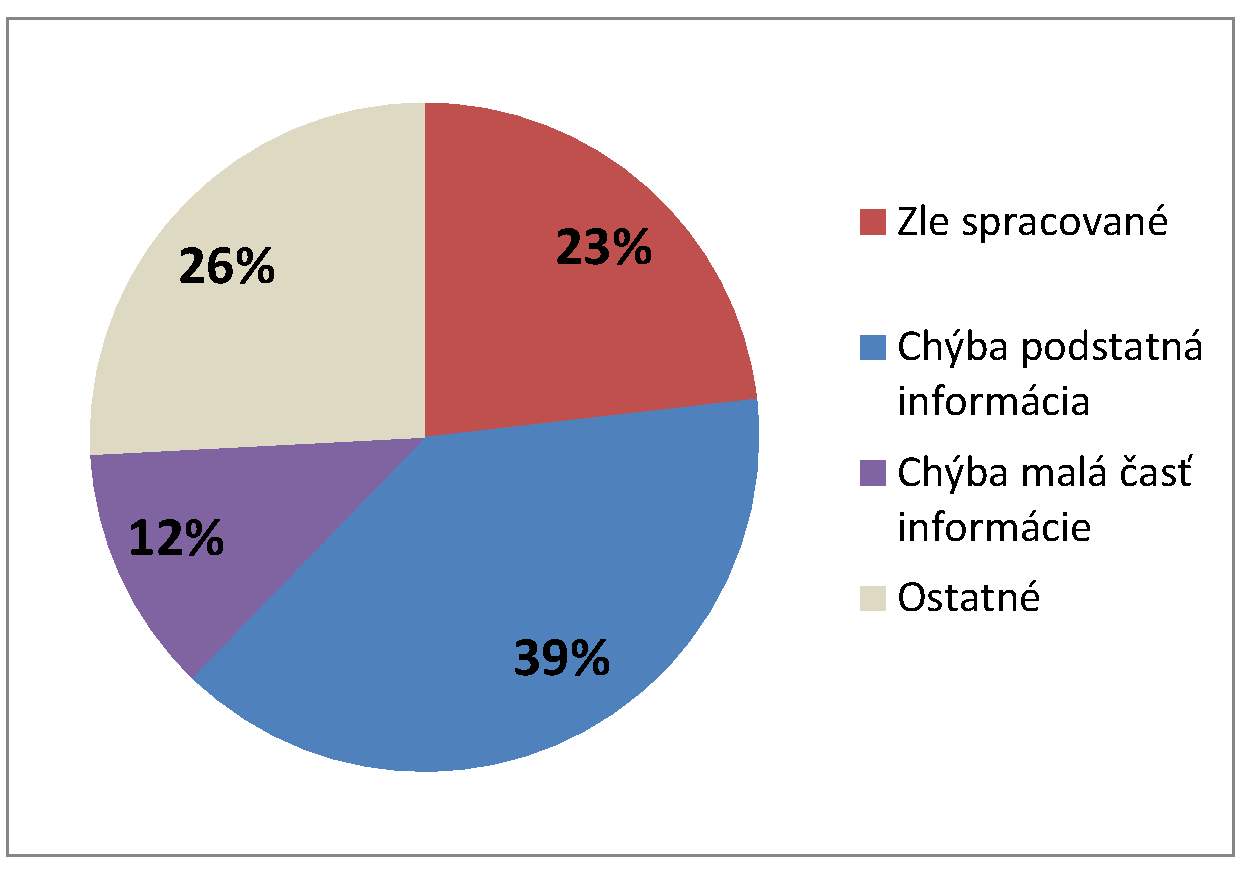
\includegraphics[scale=0.30]{exp_first_wrong} }}%
	\qquad
	\subfloat[Kategórie správnych poznámok]{{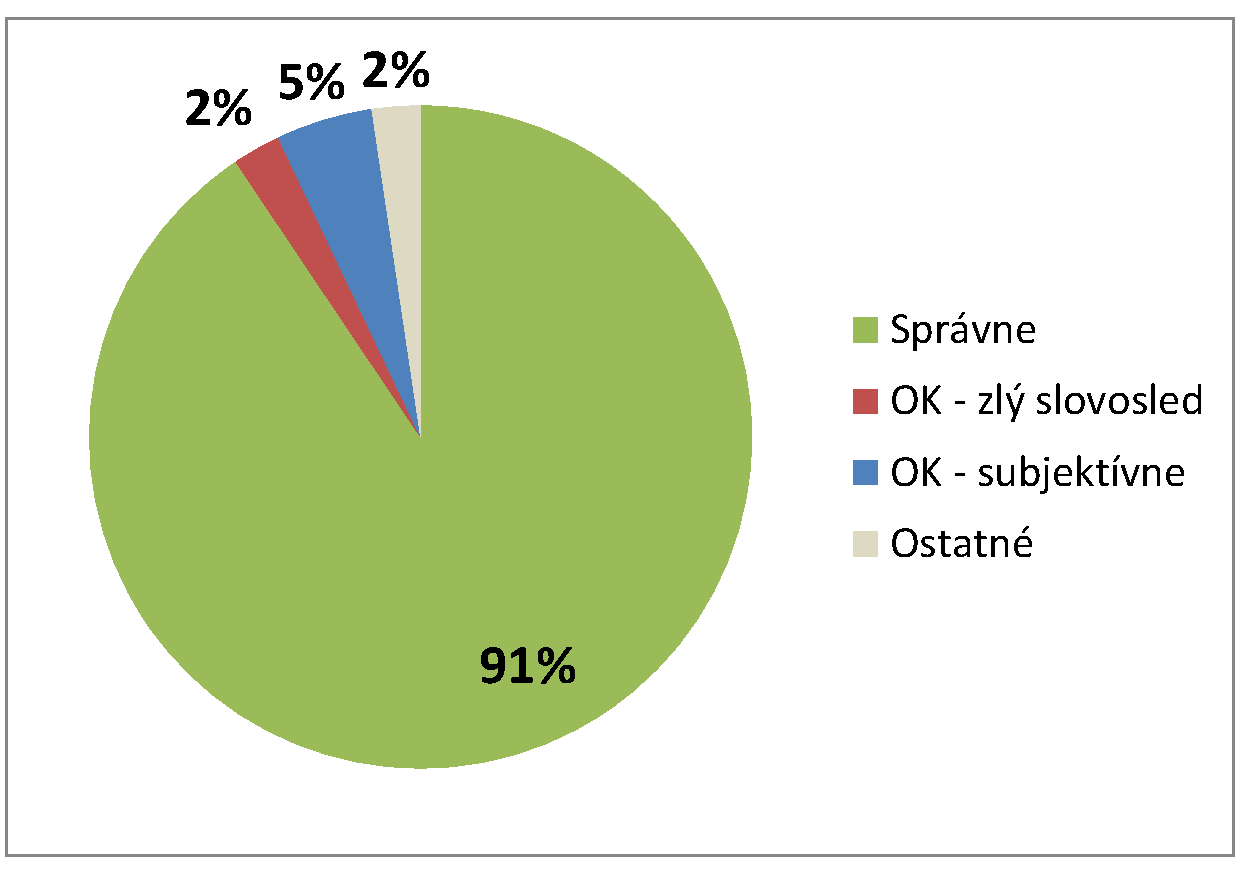
\includegraphics[scale=0.30]{exp_first_correct} }}%
	\caption{Detailné výsledky prvej časti experimentu}%
	\label{experiments:user_experiment:results:fig:exp_detailed_comparison_first}%
\end{figure}


\begin{figure}[H]%
	\centering
	\subfloat[Kategórie nesprávnych poznámok]{{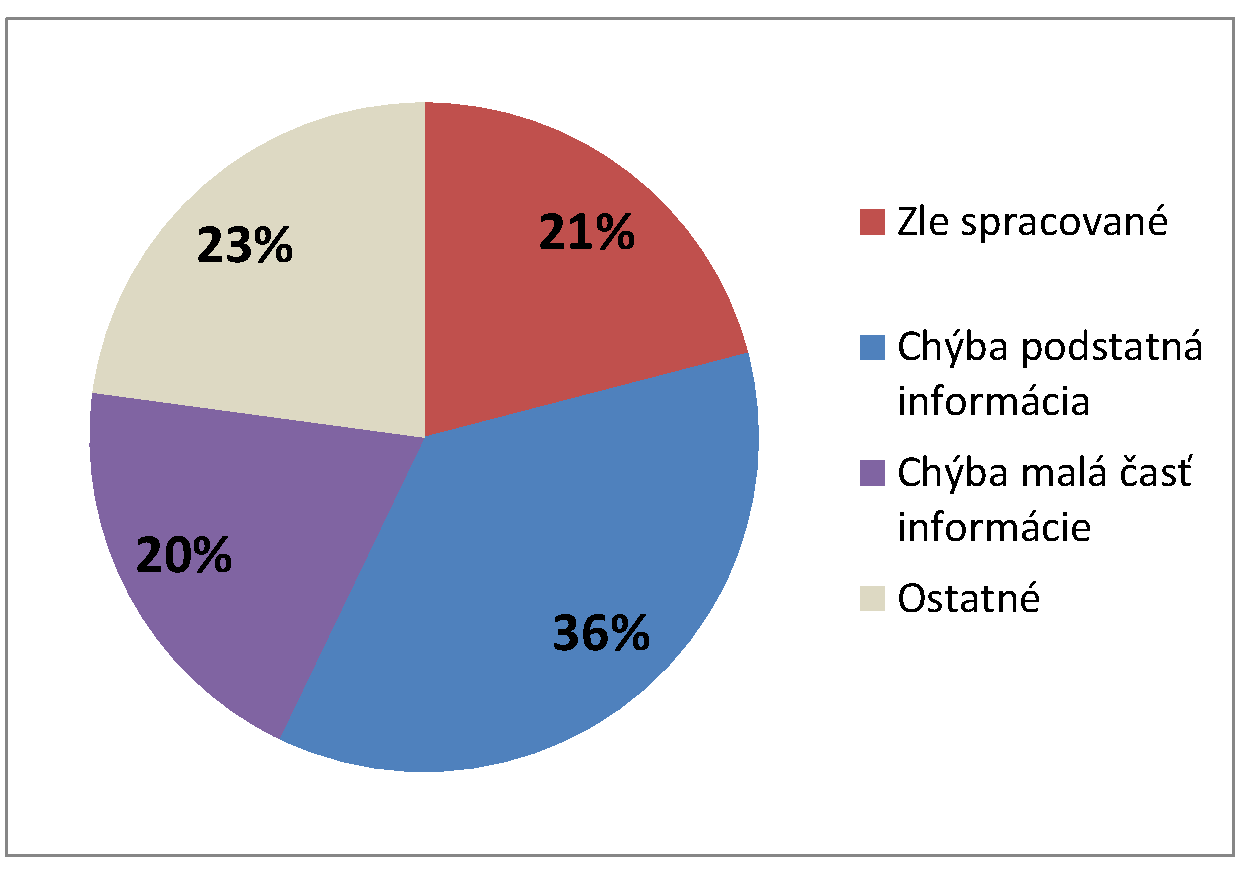
\includegraphics[scale=0.30]{exp_second_wrong} }}%
	\qquad
	\subfloat[Kategórie správnych poznámok]{{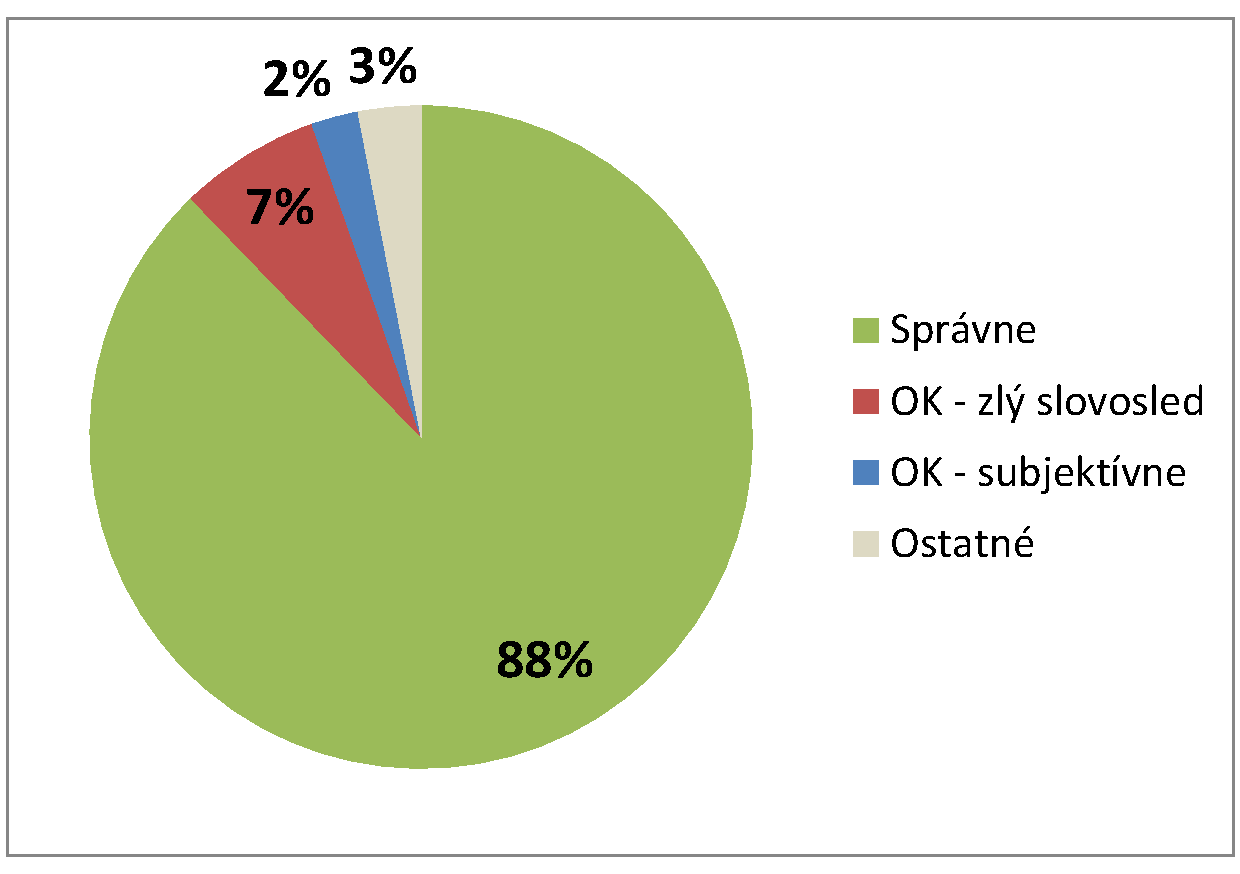
\includegraphics[scale=0.30]{exp_second_correct} }}%
	\caption{Detailné výsledky druhej časti experimentu}%
	\label{experiments:user_experiment:results:fig:exp_detailed_comparison_second}%
\end{figure}

\subsubsection{Vyhodnotenie experimentu}
Tvorba vyhovujúcich poznámok je subjektívna aktivita a preto hodnotenia účastníkov experimentu boli subjektívne a ovplyvnené ich predstavou o tvorbe poznámok. Avšak subjektívne hodnotenia boli objektívne roztriedené do kategórií a vyhodnotené. Z výsledkov je vidno $20\%$ zlepšenie z pohľadu počtu správne vytvorených poznámok pri použití databázy s väčším počtom pravidiel. V druhej časti je oproti prvej časti znížený počet zle spracovaných poznámok a poznámok, v ktorých chýbala podstatná informácia. Zväčšilo sa percentuálne zastúpenie kategórie \textit{chýba mala časť informácie}, čo naznačuje zlepšenie aj v prípade nesprávne vytvorených poznámok. V správne vytvorených poznámkach je v druhej časti väčšie percentuálne zastúpenie kategórie \textit{OK - zlý slovosled} oproti prvej časti. Taktiež nastali situácie kedy poznámka v prvej časti bola vytvorená správne a v druhej časti nesprávne. Spomenuté zhoršenia druhej časti oproti prvej súvisia s veľkou všeobecnosťou pravidla. Pravidlo sa aplikuje na vetu s rovnakou štruktúrou, ale rovnaká štruktúra môže mať viacero rôznych spracovaní.
% Z toho nám vyplynulo, že pravidlo príliš všeobecné a je potrebné aby bolo viac reštriktívne.

$80\%$ účastníkov experimentu podalo pozitívnu spätnú väzbu a vyjadrilo sa, že by takýto alebo podobný systém na tvorbu poznámok používali.

\subsection{Zhrnutie}
Na systéme boli vykonané tri experimenty. V prvom experiment sme náš systém porovnali so systémom Autosummarizer, ktorý sa špecializuje na sumarizáciu textu. Z tohto experimentu sa ukázalo, že náš systém posiela na výstup viacero viet a slov ako porovnávaný systém, čo môže mať za dôsledok veľké množstvo dát na výstupe pri rozsiahlejších článkoch. Na druhej strane náš systém spracoval všetky vety a eliminoval v nich irelevantné informácie. Druhý systém vynechal vety pri spracovávaní a tak isto neeliminoval irelevantné informácie z viet.

Druhým experimentom sme dokázali, že pravidlá sú dostatočne všeobecné, aby sa dali použiť na viacero viet s rovnakou štruktúrou. Tým sa nám podarilo ušetriť podstatnú časť prípadných pravidiel, ktoré by systém musel vytvoriť, ak by pre každú vetu potreboval samostatné pravidlo.

Pomocou používateľského experimentu sme overili systémovú závislosť od počtu pravidiel. Čím viac pravidiel má systém k dispozícií, tým kvalitnejšie spracováva vety, vytvára lepšie poznámky a stáva sa viac personalizovaný pre používateľa. Zaznamenali sme podstatné zlepšenie pri použití väčšieho množstva pravidiel v systéme. Z experimentu vyplynulo, že aj keď je poznámka spracovaná nesprávne, neznamená to, že je úplne nepoužiteľná pre používateľa. V podstatnej časti nesprávne vytvorených poznámok chýbala iba mala časť informácie z vety na to, aby bola úplne pochopiteľná a použiteľná pre používateľa. Počas experimentu sme odhalili situácie, kedy sa veta pri menšom počte pravidiel spracovala správne a pri väčšom počte nesprávne. Za dôsledok to má veľká všeobecnosť pravidla a je potrebné, aby bolo viac reštriktívne.

%%
%% Conclusion
%%tex 
\newpage
\ifthenelse {\boolean{bachelor}}
{
	\section{Conslusions}
	%\section{Záver}
}
{
	\chapter{Conclusions}
	%\chapter{Záver}
}
Lorem ipsum dolor sit amet, consectetuer adipiscing elit. Morbi sit amet arcu. Fusce pharetra dapibus elit. Duis malesuada. Proin at elit vitae quam cursus tristique. Quisque fermentum. Praesent dictum. Nullam vehicula. Nunc pharetra dolor ut velit. Sed pulvinar, est sed congue tempor, nibh arcu cursus enim, quis consequat magna lacus sed pede. In sagittis. Etiam volutpat, velit id tincidunt egestas, augue ligula auctor eros, sit amet viverra sapien tortor at odio. In diam libero, fringilla ut, adipiscing condimentum, ultricies at, dui. Phasellus vitae risus.

Pellentesque vulputate ante ut diam. Sed adipiscing malesuada odio. Pellentesque habitant morbi tristique senectus et netus et malesuada fames ac turpis egestas. Nam a leo. Praesent velit. Aenean vehicula accumsan quam. Nulla dolor lorem, imperdiet a, ullamcorper hendrerit, ultrices at, urna. Integer placerat ligula id purus. Sed id nisl. Pellentesque tincidunt neque in lacus. In non quam et felis suscipit viverra.

%%
%% References
%%
\newpage
\addcontentsline{toc}{section}{\refname}
\bibliographystyle{plain}
\bibliography{references}

%%
%% Appendix
%%
\ifthenelse {\boolean{bachelor}}
{
}
{
	\ifthenelse {\boolean{english}}
	{
		\renewcommand{\appendixname}{Appendix}
		\renewcommand{\appendixtocname}{Appendix}
	}
	{
		\renewcommand{\appendixname}{Príloha}
		\renewcommand{\appendixtocname}{Prílohy}
	}
	\pagenumbering{bychapter}
}
\appendix
%\newpage
%\thispagestyle{plain}
%\ifthenelse {\boolean{bachelor}}
%{
%	%\section{Technical documentation}
%	\section{Technická dokumentácia}
%}
%{
%	%\chapter{Technical documentation}
%	\chapter{Technická dokumentácia}
%}
% \label{technical_documentation}
%Lorem ipsum dolor sit amet, consectetuer adipiscing elit, sed diam nonummy nibh euismod tincidunt ut laoreet dolore magna aliquam erat volutpat. Ut wisi enim ad minim veniam, quis nostrud exerci tation ullamcorper suscipit lobortis nisl ut aliquip ex ea commodo consequat. 
%\ifthenelse {\boolean{bachelor}}
%{
%	%\subsection{Implementation}
%	\subsection{Implementácia}
%}
%{
%	%\section{Implementation}
%	\section{Implementácia}
%}
%\paragraph{Modul abc}
%Lorem ipsum dolor sit amet, consectetuer adipiscing elit, sed diam nonummy nibh euismod tincidunt ut laoreet dolore magna aliquam erat volutpat. Ut wisi enim ad minim veniam, quis nostrud exerci tation ullamcorper suscipit lobortis nisl ut aliquip ex ea commodo consequat. Duis autem vel eum iriure dolor in hendrerit in vulputate velit esse molestie consequat, vel illum dolore eu feugiat nulla facilisis at vero eros et accumsan et iusto odio dignissim qui blandit praesent luptatum zzril delenit augue duis dolore te feugait nulla facilisi. Nam liber tempor cum soluta nobis eleifend option congue nihil imperdiet doming id quod mazim placerat facer possim assum.
%\paragraph{Modul def}
%Lorem ipsum dolor sit amet, consectetuer adipiscing elit, sed diam nonummy nibh euismod tincidunt ut laoreet dolore magna aliquam erat volutpat. Ut wisi enim ad minim veniam, quis nostrud exerci tation ullamcorper suscipit lobortis nisl ut aliquip ex ea commodo consequat. Duis autem vel eum iriure dolor in hendrerit in vulputate velit esse molestie consequat, vel illum dolore eu feugiat nulla facilisis at vero eros et accumsan et iusto odio dignissim qui blandit praesent luptatum zzril delenit augue duis dolore te feugait nulla facilisi. Nam liber tempor cum soluta nobis eleifend option congue nihil imperdiet doming id quod mazim placerat facer possim assum. Typi non habent claritatem insitam; est usus legentis in iis qui facit eorum claritatem. Investigationes demonstraverunt lectores legere me lius quod ii legunt saepius. Claritas est etiam processus dynamicus, qui sequitur mutationem consuetudium lectorum. Mirum est notare quam littera gothica, quam nunc putamus parum claram, anteposuerit litterarum formas humanitatis per seacula quarta decima et quinta decima. Eodem modo typi, qui nunc nobis videntur parum clari, fiant sollemnes in futurum.
\newpage
\ifthenelse {\boolean{bachelor}}
{
	%\section{User documentation}
	\section{Používateľská príručka}
}
{
	%\chapter{User documentation}
	\chapter{Dokumentácia}
}

\subsection{Inštalácia}
Nástroj nie je potrebné inštalovať. Na elektronickom médiu sa nachádza spustiteľný súbor \textit{Notenizer.exe}, ktorý spustí systém.

\subsection{Spustenie systému}
Systém ponúka prácu cez dve rozhrania - príkazový riadok a grafické používateľské rozhranie. Na príkazovom riadku nie su dostupné všetky vymoženosti systému, ako napríklad interaktívna úprava poznámok. Podľa zadaných argumentov sa spustenie a správanie systému prispôsobuje.

\subsubsection{Možnosti spustenia systému}
\begin{table}[H]
	\centering
	\caption{Argumenty systému}
	\label{appendix:run:table:arguments}
	\begin{tabular}{|l|l|l|}
		\hline
		\textbf{Argument} & \textbf{Vykonaná akcia} & \textbf{Predvolené} \\ \hline
		-t, \hyph\hyph text & Text, ktorý sa má spracovať & \\ \hline
		\hyph\hyph url & URL adresa článku na wikipédií & \\ \hline
		\hyph\hyph country & Spracuje článok o krajine z wikipédie & \\ \hline
		-v & Zobrazí ladiace a pomocné výpisy programu & false \\ \hline
		-c & Program zbehne jednorázovo na príkazovom riadku & false \\ \hline
		\hyph\hyph analyze & Vykoná analýzu nad súčasnou databázou & false \\ \hline
		-d, \hyph\hyph db & Názov databázy, ku ktorej sa pripojí & notenizer\\ \hline
		-h, \hyph\hyph host & Názov servera, ku ktorému sa pripojí & localhost \\ \hline
		-p, \hyph\hyph port & Port na ktorom počúva MongoDB databáza & 27017 \\ \hline
		-u & Meno databázového používateľa & \\ \hline
		\hyph\hyph password & Heslo databázového používateľa & \\ \hline
		\hyph\hyph help & Zobrazí túto pomocnú správu & \\ \hline
	\end{tabular}
\end{table}

\subsection{Používateľské rozhranie}

Hlavné okno aplikácie (\imgref{appendix:gui:main_window}) pozostáva zo štyroch častí:
\begin{my_enumerate}
	\item menu File (\imgref{appendix:gui:menu_file}),
	\item menu Edit (\imgref{appendix:gui:menu_edit}),
	\item priestor na pôvodné vety,
	\item priestor na poznámky,
	\item zobrazí okno na editovanie poznámky (\imgref{appendix:gui:edit_window})
\end{my_enumerate}

\begin{figure}[H]
	\begin{center}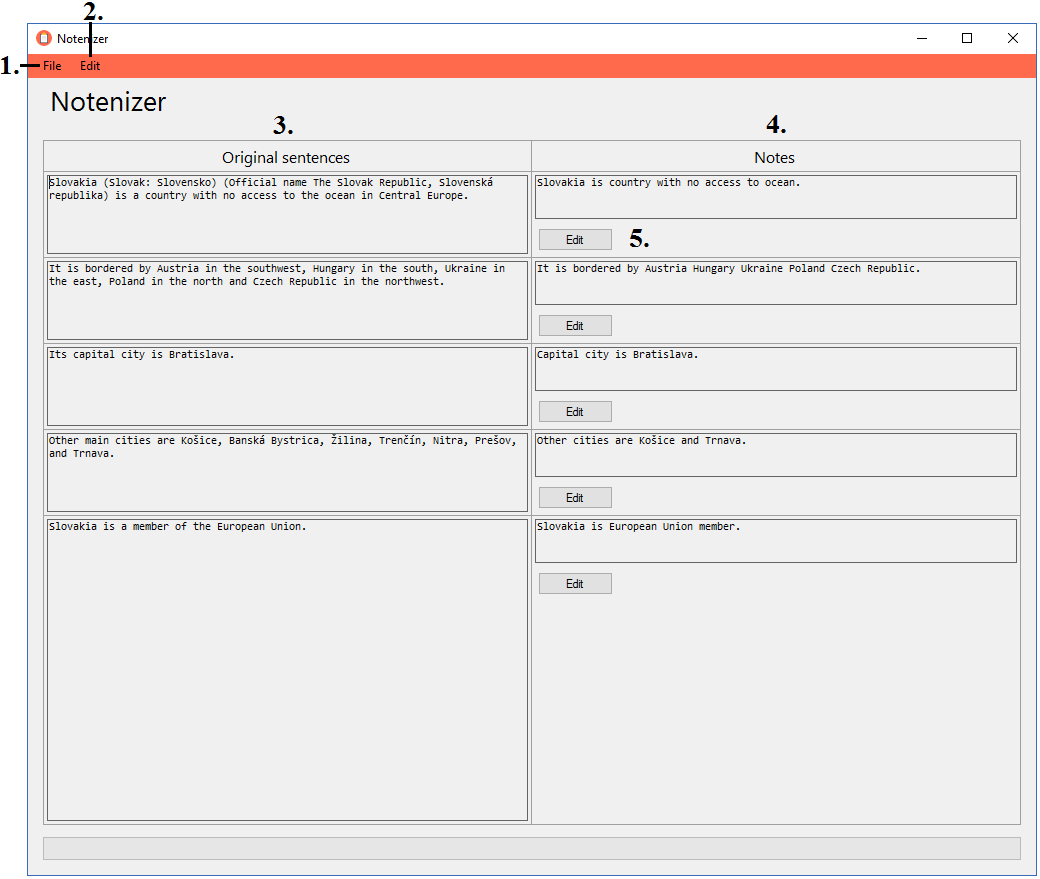
\includegraphics[scale=0.5]{gui_main_window}\end{center}
	\caption[Grafické rozhranie - Hlavné okno]{Grafické rozhranie - Hlavné okno}\label{appendix:gui:main_window}
\end{figure}

Menu File (\imgref{appendix:gui:menu_file}) ponúka viacero operácií s textami:
\begin{my_enumerate}
	\item otvorí okno pre načítanie textu na spracovanie (\imgref{appendix:gui:input_window}),
	\item získa text na spracovanie zo zvoleného textového súboru,
	\item zobrazí okno na dotiahnutie textu z wikipédie (\imgref{appendix:gui:link_window}),
	\item uloží vytvorené poznámky do textového súboru,
	\item ukončí program.
\end{my_enumerate}

\begin{figure}[H]
	\begin{center}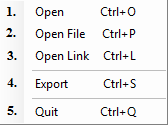
\includegraphics[scale=1]{gui_menu_file}\end{center}
	\caption[Grafické rozhranie - Menu File]{Grafické rozhranie - Menu File}\label{appendix:gui:menu_file}
\end{figure}

Menu Edit (\imgref{appendix:gui:menu_edit}) ponúka operácie:
\begin{my_enumerate}
	\item zo zobrazovacej plochy odstráni pôvodne vety a poznámky.
\end{my_enumerate}

\begin{figure}[H]
	\begin{center}
\includegraphics[scale=1]{gui_menu_edit}\end{center}
	\caption[Grafické rozhranie - Menu Edit]{Grafické rozhranie - Menu Edit}\label{appendix:gui:menu_edit}
\end{figure}

Okno na načítanie textu na spracovanie (\imgref{appendix:gui:input_window}) obsahuje:
\begin{my_enumerate}
	\item textovú plochu na načítanie textu na spracovanie.
\end{my_enumerate}
\begin{figure}[H]
	\begin{center}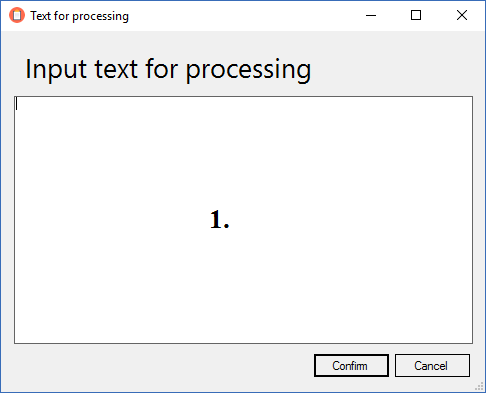
\includegraphics[scale=0.6]{gui_input_text}\end{center}
	\caption[Grafické rozhranie - Okno na načítanie textu]{Grafické rozhranie - Okno na načítanie textu}\label{appendix:gui:input_window}
\end{figure}

Okno na dotiahnutie textu (\imgref{appendix:gui:link_window}) sa skladá z:
\begin{my_enumerate}
	\item výber dotiahnutia textu cez URL článku na wikipédií,
	\item výber dotiahnutia text z článku na wikipédií podľa názvu krajiny,
	\item zadanie URL alebo názvu krajiny.
\end{my_enumerate}
\begin{figure}[H]
	\begin{center}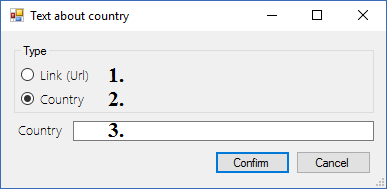
\includegraphics[scale=0.7]{gui_link_window}\end{center}
	\caption[Grafické rozhranie - Okno na dotiahnutie textu]{Grafické rozhranie - Okno na dotiahnutie textu}\label{appendix:gui:link_window}
\end{figure}

Editovacie okno poznámky (\imgref{appendix:gui:edit_window}) obsahuje prvky:
\begin{my_enumerate}
	\item znenie pôvodnej vety,
	\item znenie poznámky,
	\item interaktívne upraviteľný tvar poznámky,
	\item slová z pôvodnej vety nepoužité v poznámke,
	\item spoznámkovávač viacnásobných poznámok (\imgref{appendix:gui:andparser_window}).
\end{my_enumerate}
\begin{figure}[H]
	\begin{center}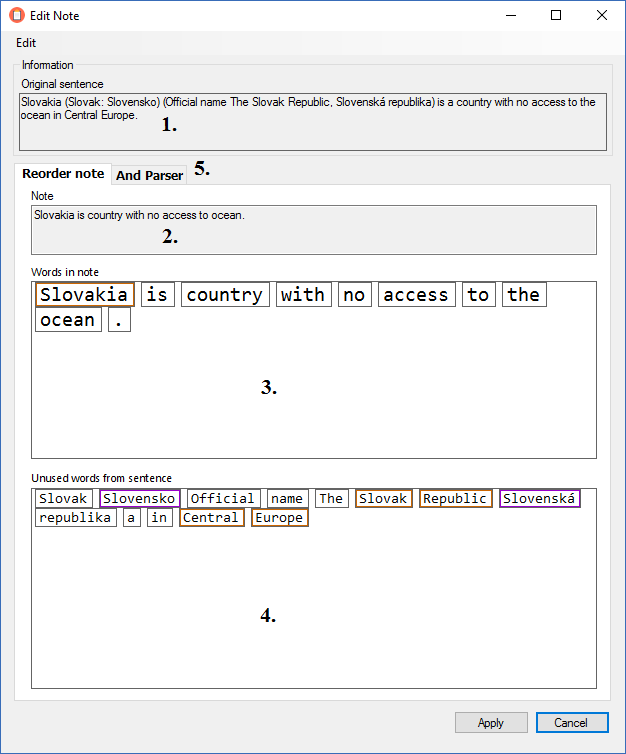
\includegraphics[scale=0.7]{gui_edit_window}\end{center}
	\caption[Grafické rozhranie - Editovacie okno poznámky]{Grafické rozhranie - Editovacie okno poznámky}\label{appendix:gui:edit_window}
\end{figure}

Editovacie okno viacnásobných poznámok (\imgref{appendix:gui:andparser_window}) ponúka:
\begin{my_enumerate}
	\item znenie pôvodnej vety,
	\item viacnásobnú poznámku,
	\item interaktívne upraviteľný tvar viacnásobnej poznámky,
	\item slová z pôvodnej vety nepoužité vo viacnásobnej poznámke,
	\item špeciálny prvok označujúci množinu viacnásobnej poznámky.
\end{my_enumerate}
\begin{figure}[H]
	\begin{center}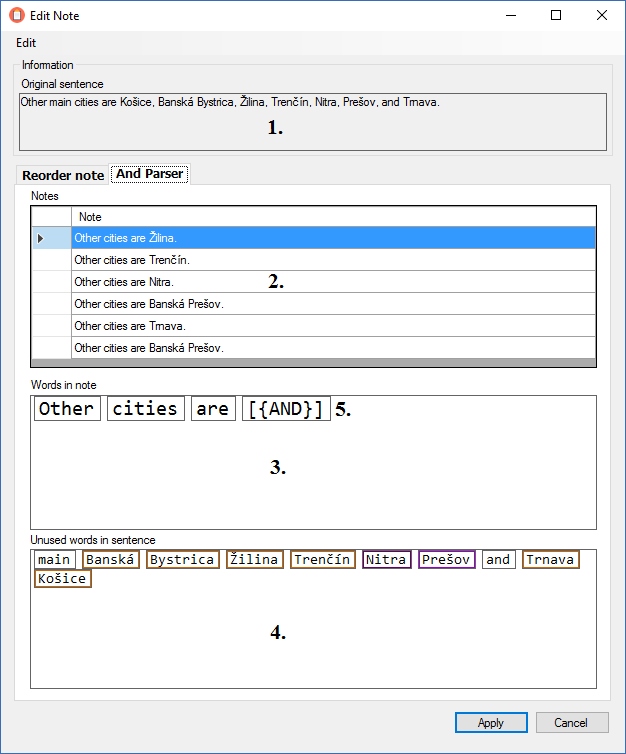
\includegraphics[scale=0.7]{gui_andparser_window}\end{center}
	\caption[Grafické rozhranie - Editovacie okno viacnásobných poznámok]{Grafické rozhranie - Editovacie okno viacnásobných poznámok}\label{appendix:gui:andparser_window}
\end{figure}

%\\
%\newpage
%\ifthenelse {\boolean{bachelor}}
%{
%	%\section{Electronic medium}
%	\section{Electronické médium}
%}
%{
%	%\chapter{Electronic medium}
%	\chapter{Electronické médium}
%}
%Lorem ipsum dolor sit amet, consectetuer adipiscing elit, sed diam nonummy nibh euismod tincidunt ut laoreet dolore magna aliquam erat volutpat:
%\begin{my_itemize}
%\emptyitem /Application
%	\begin{my_itemize}
%	\myitem implementácia opisovaného riešenia
%	\end{my_itemize}	
%\emptyitem /Documentation
%	\begin{my_itemize}
%	\myitem bakalárska práca spolu s anotáciami v slovenskom a anglickom jazyku
%	\end{my_itemize}
%\emptyitem /Documentation/Latex
%	\begin{my_itemize}
%	\myitem latex zdrojové súbory dokumentácie
%	\end{my_itemize}
%\emptyitem /Documentation/BibTeX
%	\begin{my_itemize}
%	\myitem BibTeX súbor s použitými referenciami
%	\end{my_itemize}
%\emptyitem /Documentation/Resources
%	\begin{my_itemize}
%	\myitem dostupné použité zdroje
%	\end{my_itemize}
%\emptyitem /Resources
%	\begin{my_itemize}
%	\myitem vstupne/testovacie dáta opisované v dokumente
%	\end{my_itemize}
%\emptyitem /Source/Dependencies
%	\begin{my_itemize}
%	\myitem inštalačné súbory pre knižnice, ktoré potrebuje aplikácia
%	\end{my_itemize}	
%\emptyitem read.me	- popis obsahu média v slovenskom a~anglickom jazyku
%\end{my_itemize}

\newpage
\ifthenelse {\boolean{bachelor}}
{
	%\section{Electronic medium}
	\section{Zoznam vzťahov závislostí}
}
{
	%\chapter{Electronic medium}
	\chapter{Zoznam vzťahov závislostí}
}
V nasledujúcej tabuľke sú zobrazené skratky vzťahov závislostí slov vo vete ako sa používajú v programe, s celým názvom, vysvetlením, príkladom vety a použitím vzhľadom na príkladovú vetu.

\begin{figure}[H]
	\begin{center}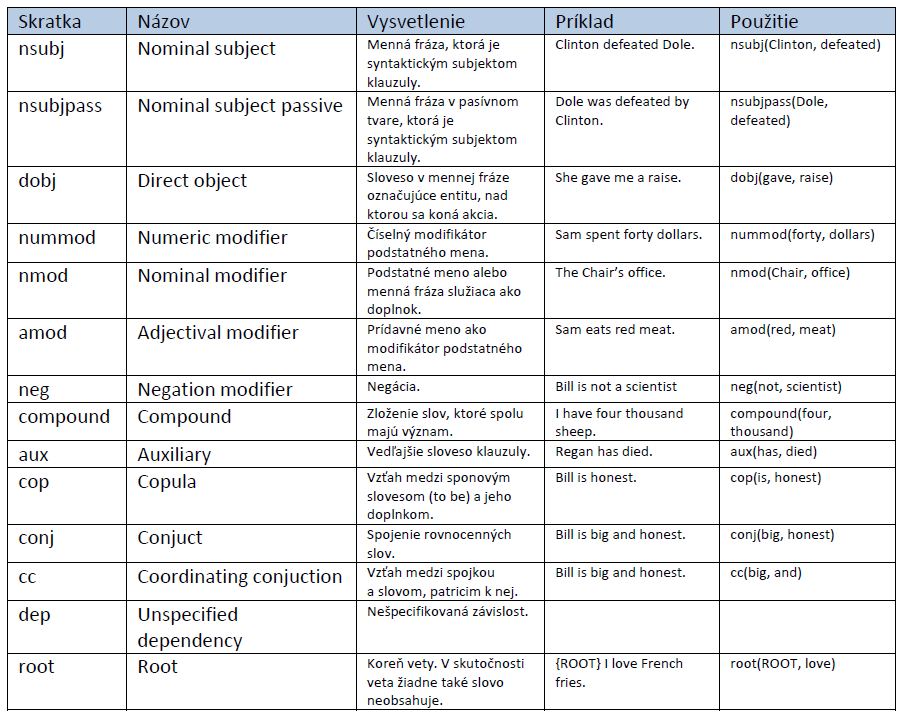
\includegraphics[scale=0.6]{dependencies_table}\end{center}
	\caption[Zoznam závislotí]{Zoznam závislostí}\label{fig:dependencies_table}
\end{figure}

\newpage
\ifthenelse {\boolean{bachelor}}
{
	%\section{Electronic medium}
	\section{Legenda diagramov kolekcií}
}
{
	%\chapter{Electronic medium}
	\chapter{Legenda diagramov kolekcií}
}
V priloženej tabuľke je legenda pre diagramy zobrazujúce štruktúru dát ukladaných v kolekciách v databáze.

\begin{figure}[H]
	\begin{center}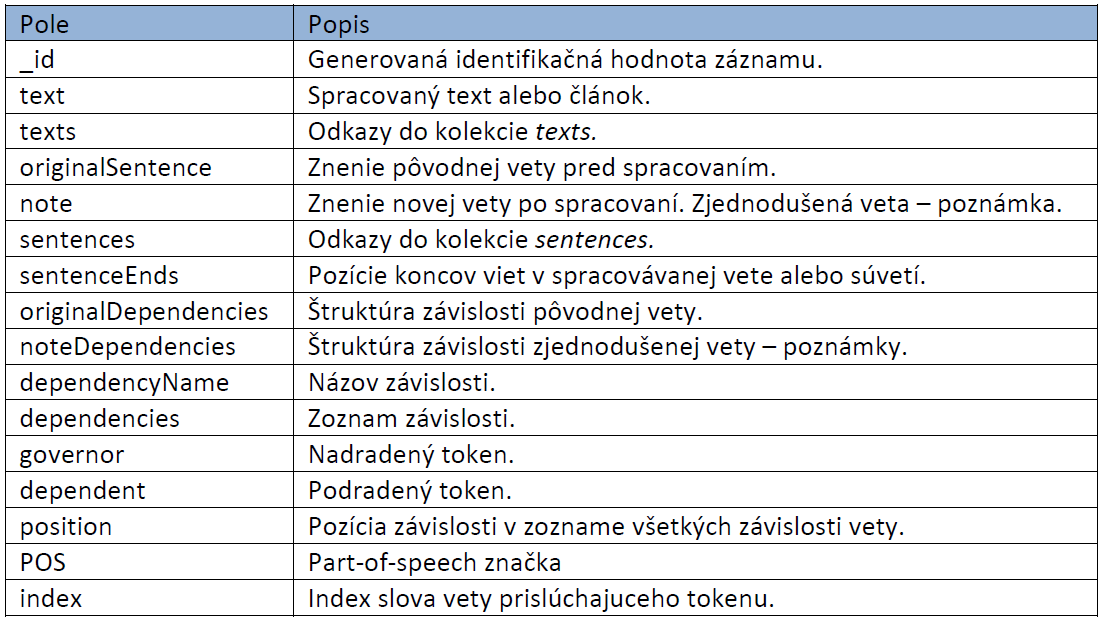
\includegraphics[scale=0.40]{collections_legend}\end{center}
	\caption[Legenda diagramov kolekcií]{Legenda diagramov kolekcií}\label{fig:collections_legend}
\end{figure}

\begin{figure}[H]
	\begin{center}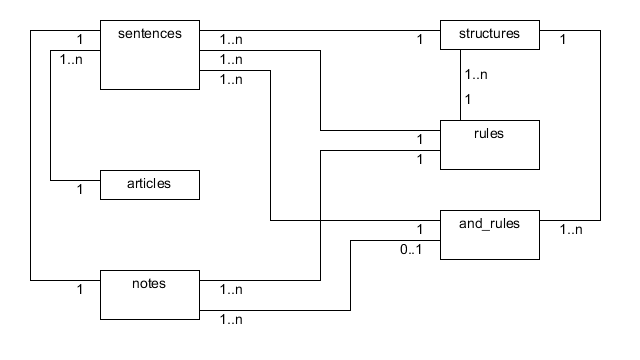
\includegraphics[scale=0.60]{db_schema}\end{center}
	\caption[Databázový model]{Databázový model}
\end{figure}

\begin{figure}[H]
	\begin{center}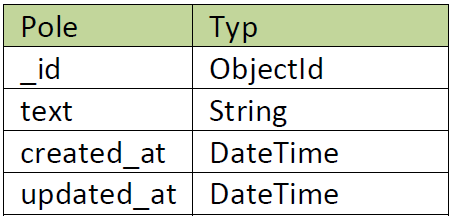
\includegraphics[scale=0.40]{articles_model}\end{center}
	\caption[Model kolekcie articles]{Model kolekcie articles}
\end{figure}

\begin{figure}[H]
	\begin{center}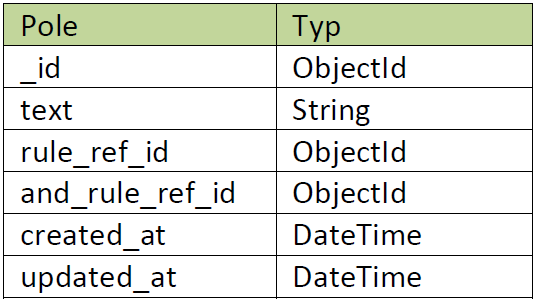
\includegraphics[scale=0.40]{notes_model}\end{center}
	\caption[Model kolekcie notes]{Model kolekcie notes}\label{fig:notes_collection_model}
\end{figure}

\begin{figure}[H]
	\begin{center}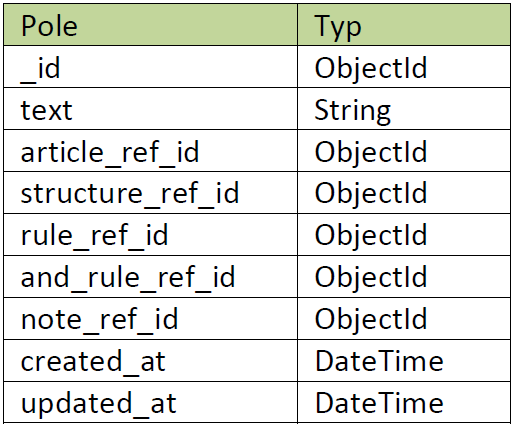
\includegraphics[scale=0.42]{sentences_model}\end{center}
	\caption[Model kolekcie sentences]{Model kolekcie sentences}\label{fig:sentences_collection_model}
\end{figure}

\begin{figure}[H]
	\begin{center}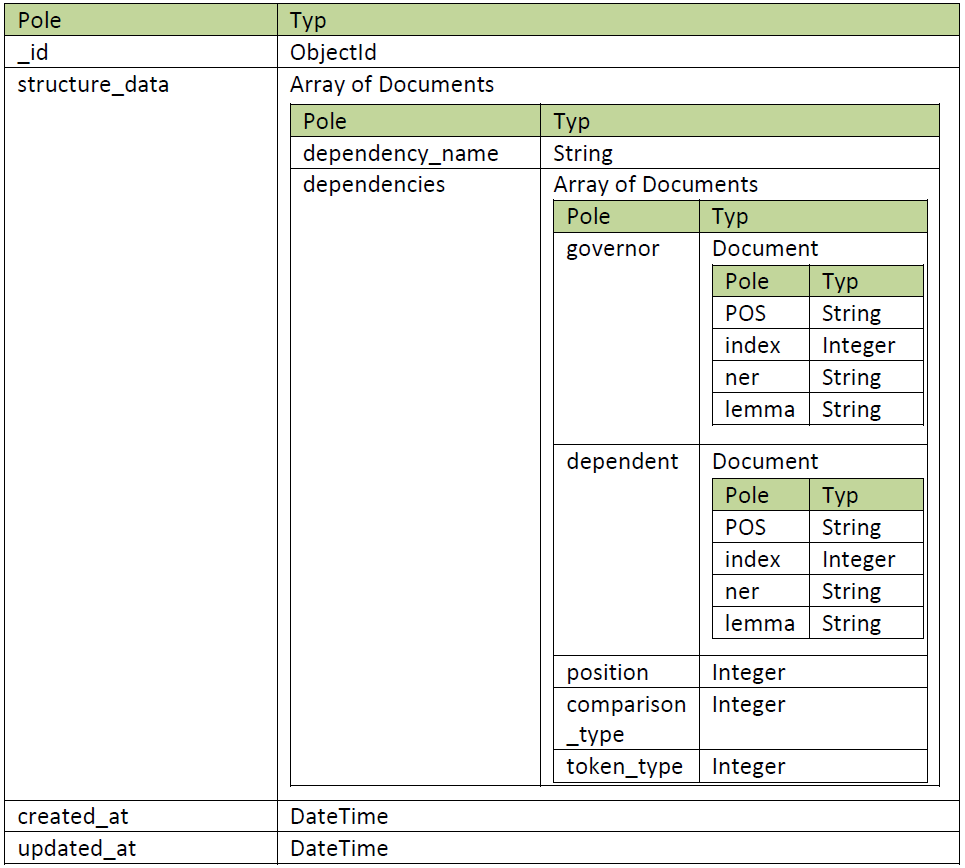
\includegraphics[scale=0.48]{structure_model}\end{center}
	\caption[Model kolekcie structures]{Model kolekcie structures}\label{fig:structures_collection_model}
\end{figure}

\begin{figure}[H]
	\begin{center}\includegraphics[scale=0.40]{rules_model}\end{center}
	\caption[Model kolekcie rules]{Model kolekcie rules}\label{fig:rules_collection_model}
\end{figure}

\begin{figure}[H]
	\begin{center}\includegraphics[scale=0.40]{and_rules_model}\end{center}
	\caption[Model kolekcie and rules]{Model kolekcie and rules}\label{fig:and_rules_collection_model}
\end{figure}

\newpage
\ifthenelse {\boolean{bachelor}}
{
	%\section{Electronic medium}
	\section{Ukážka článkov použitých v experimente}
}
{
	%\chapter{Electronic medium}
	\chapter{Legenda diagramov kolekcií}
}
\textit{Slovensko} - ,,Slovakia (Slovak: Slovensko) (Official name The Slovak Republic, Slovenská republika) is a country with no access to the ocean in Central Europe. It is bordered by Austria in the southwest, Hungary in the south, Ukraine in the east, Poland in the north and Czech Republic in the northwest. Its capital city is Bratislava. Other main cities are Košice, Banská Bystrica, Žilina, Trenčín, Nitra, Prešov, and Trnava. Slovakia is a member of the European Union.'' \\

\noindent
\textit{Česko} - ,,Czech Republic (Czech: Česká republika) is a country in Central Europe, sometimes also known as Czechia (Czech: Česko). The capital and the biggest city is Prague. The currency is the Czech Crown (koruna česká - CZK). 1€ is about 27 CZK. The president of the Czech Republic is Miloš Zeman. The Czech Republic's population is about 10.5 million. The local language is Czech language. The Czech language is a Slavic language. It is related to languages like Slovak and Polish. In 1993 the Czech Ministry of Foreign Affairs announced that the name Czechia be used for the country outside of formal official documents. This has not caught on in English usage. Czech Republic has no sea; its neighbour countries are Germany, Austria, Slovakia, and Poland.'' \\

\noindent
\textit{Maďarsko} - ,,Hungary is a country in Central Europe. Its capital city is Budapest. Hungary is slightly bigger than its western neighbour Austria and has about 10 million inhabitants. Other countries that border Hungary are Slovakia, Ukraine, Romania, Serbia, Croatia and Slovenia. Hungary's official language is the Hungarian language. It has been a member of the European Union (EU) since 2004. In Hungarian the country is called Magyarország (Hungary) or Magyar Köztársaság (Hungarian Republic). This is named after the Magyar tribes who came to Hungary in the late 9th century.'' \\

\noindent
\textit{Poľsko} - ,,Poland is a country in Eastern Europe. It is next to Germany to the west (along Oder and Lusatian Neisse), the Czech Republic and Slovakia to the south, Ukraine and Belarus to the east, and the Baltic Sea, Lithuania, and Russia to the north. The total land area of Poland is about 312,679 km2 (120,728 mi2). This makes Poland the 77th largest country in the world with over 38.5 million people. Most Polish people live in large cities, including the capital, Warsaw (Polish: Warszawa), Łódź, Cracow (Polish: Kraków), the second capital of Poland (first was Gniezno), Szczecin, Gdańsk, Wrocław and Poznań. The word "Poland" was written officially for the first time in 966. In 1569, Poland formed a strong union with Lithuania called the Polish-Lithuanian Commonwealth. At some point in its history, it was the largest state in Europe and became very influential. Much of the territory that now makes up Central European states used to belong to the Commonwealth. Eventually, after entering a somewhat sudden yet steady decline, the Commonwealth collapsed in 1795. Poland regained its independence in 1918 after World War I. In 1921, Poland defeated Soviet Russia in the Polish-Soviet War that started in 1919.'' \\

\noindent
\textit{Nemecko} - ,,The Federal Republic of Germany, also called Germany (German: Bundesrepublik Deutschland or just Deutschland), is a country in Central Europe. The country's full name is sometimes shortened to the FRG (or the BRD, in German). To the north of Germany are the North Sea, the Baltic Sea, and the country of Denmark. To the east of Germany are the countries of Poland and the Czech Republic. To the south of Germany are the countries of Austria and Switzerland. To the west of Germany are the countries of France, Luxembourg, Belgium, and the Netherlands. The total area of Germany is 137,847 square miles. The large majority of Germany has warm summers and cool or cold winters. In June 2013, Germany had a population of 80.6 million people. After the United States, Germany is the second most popular country for migration in the world. Before it was called Germany, it was called Germania. In the years A.D. 900 until 1806, Germany was part of the Holy Roman Empire. From 1949 to 1990, Germany was made up of two countries called the Federal Republic of Germany (inf. West Germany) and the German Democratic Republic (inf. East Germany). During this time, the capital city of Berlin was divided into a west and an east part. On 13 August 1961, East Germany started building the Berlin Wall between the two parts of Berlin. West Germany was one of the countries that started the European Union.'' \\

\noindent
\textit{Taliansko} - ,,Italy is a country in Europe and a member of the European Union. Its official name is Repubblica Italiana. Italy is a democratic republic and is a founding member of the European Union. Italy is also a member of the G8, as it has the 8th largest Gross Domestic Product in the world. Its President is Sergio Mattarella and its Prime Minister is Matteo Renzi. Before 1861, it was made up of smaller kingdoms and city-states.'' \\

\noindent
\textit{Francúzsko} - ,,France (French: France), officially the French Republic (French: République française), is a country in Western Europe. Its capital city is Paris. It is a member of the European Union. It is known for its culture, its many monuments and structures, and places such as the Louvre, the Eiffel Tower, the Arc de Triomphe, Giverny, Mont Saint Michel, Versailles, and Notre Dame de Paris. France is divided into 22 régions that are further subdivided départements. The country has been one of the great powers since the end of the 17th century. In the 18th and 19th centuries, it built a big colonial empire across West Africa and Southeast Asia. Nowadays, this does not exist. It is the most visited country in the world. About 82 million foreign tourists visit it every year. France is a founding member of the European Union. It has the largest land area of any member. France is also a founding member of the United Nations, and a member of the G8 and NATO. It is one of the five permanent members of the United Nations Security Council. It has nuclear weapons, including active warheads, and also has nuclear power plants. Some well-known cities in France include Paris, Lyon, Marseille, Bordeaux, Lille, Toulouse, Nice, Strasbourg, Rennes and Nantes.'' \\

\noindent
\textit{Spojené kráľovstvo} - ,,The United Kingdom of Great Britain and Northern Ireland, called the United Kingdom, GB or UK, is a sovereign state in Western Europe. It unites England, Northern Ireland, Scotland and Wales as one Kingdom.[10] It is a member of the European Union, the United Nations, the Commonwealth, NATO and the G8. It has the sixth largest economy in the world. Around 65 million people live in the UK. Most people in the UK speak English. There are five native languages other than English. They are Welsh in Wales, Gaelic and Scots in Scotland and Northern Ireland, Irish in Northern Ireland, and Cornish in Cornwall. Between the 17th and mid 20th-centuries Britain was an important world power. It became a colonial empire that controlled large areas of Africa, Asia, North America and Oceania. Today this empire does not exist, although Britain keeps links with most countries of its former empire. Some well-known cities in the UK are London, Edinburgh, Cardiff, Belfast, Manchester, Bristol, Liverpool, Birmingham, York and Glasgow.'' \\

\noindent
\textit{Španielsko} - ,,Spain is a country in Southern Europe. It is in the Iberian Peninsula near Portugal and Gibraltar. France and the country of Andorra are on its northeast side, where the Pyrenees mountains are. The people of Spain are called Spaniards. Most people there speak Spanish (in Spanish, "Castellano", from Castilla, or "Español") but there are other languages in different parts of the country. They are Catalan, Basque, and Galician, Leonese, Aragonese, Aranese Occitan and even Portuguese. The religion of most of the people in Spain is Roman Catholic. Since 1975, Spain has had a king who only does what the constitution allows him to. For example, the king can declare a war, but only if the Government asks him to do so. The parliament is called Las Cortes Generales, and has two bodies: "El Congreso" (The Congress) and "El Senado" (The Senate) and it is chosen by the Spanish people by voting. This kind of government is called a constitutional monarchy. The King of Spain is Felipe VI. The Prime minister is Mariano Rajoy. The government and the king's palace are in Madrid, the capital of Spain. Spain has more than five hundred thousand square kilometres of land. It is smaller than France, but it is bigger than Sweden or Germany. Almost fifty million people live in Spain. Spain has 17 parts called autonomous communities (this means that they can decide upon some affairs themselves). Each part has its own government.'' \\

\noindent
\textit{Ukrajina} - ,,Ukraine is a country in Eastern Europe. Russia is to the north-east of Ukraine, Belarus is to the Northwest, Poland and Slovakia are to the West, Hungary, Romania, Moldova and self-proclaimed Transnistria are to the South West and the Black Sea is to the Southwest. Ukraine is a republic. The capital of Ukraine is Kiev. It was a part of the Soviet Union from 1922 until 1991.'' \\

\noindent
\textit{Rakúsko} - ,,Austria (German: Österreich; officially called Republic of Austria), is a country in Central Europe. Around Austria there are Germany, Czech Republic, Slovakia, Hungary, Slovenia, Italy, Switzerland, and Liechtenstein. Currently, the chancellor is Werner Faymann. Austria has been a member-state of the EU since 1995. The people in Austria speak German, a few also Hungarian, Slovenian and Croatian. The capital of Austria is Vienna (Wien). Austria is more than a thousand years old. Its history can be followed to the ninth century. At that time the first people moved to the land now known as Austria. The name "Ostarrichi" is first written in an official document from 996. Since then this word has developed into the Modern German word Österreich, which literally means "East Kingdom." Austria is a democratic state and has nine federal states (German: 'Bundesländer'): Vorarlberg, the Tyrol, Salzburg, Carinthia, Styria, Upper Austria, Lower Austria, Vienna and Burgenland. It is a neutral state, that means it does not take part in wars with other countries. Austria has been in the United Nations since 1955 and in the European Union since 1995.'' \\

\noindent
\textit{Švédsko} - ,,Sweden (Swedish: Sverige) is a Nordic country in the part of Europe called Scandinavia. Its neighbors are Finland and Norway. Sweden is also connected to Denmark in the south by a bridge. It is a developed country. It is famous for its welfare state. People who live in Sweden are called Swedes. Sweden's capital city is Stockholm. Sweden is a constitutional monarchy because it has a king, Carl XVI Gustaf, but he does not have any real power. Sweden is a parliamentary state meaning that the government is elected by the parliament which is appointed by the people. The country is democratically ruled by a government headed by an elected prime minister. Stefan Löfven was elected Prime Minister in September 2014. He took office in October 2014. The population of Sweden is almost 9.5 million people. Sweden has an official majority language, (called svenska in Swedish). Sweden has five official minority languages, Finnish, Yiddish, Sami, Meänkieli and Romani. Sweden became a member of the European Union in 1995. It is not a member of the Eurozone. Sweden has not begun to use the euro as currency. This is because the people have voted against this. The currency remains the Swedish krona (Swedish crown). Sweden has 25 provinces (landskap). They are found in three different regions: Norrland in the North, Svealand, the central region, and Götaland in the South.''

\newpage
\ifthenelse {\boolean{bachelor}}
{
	%\section{Electronic medium}
	\section{IIT.SRC článok}
}
{
	%\chapter{Electronic medium}
	\chapter{Legenda diagramov kolekcií}
}
\includepdf[pages={1,2,3}, pagecommand={}]{interactive_system_for_creation_of_notes.pdf}


\end{document}

%%%%%%%%%%%%%%%%%%%%%%%%%%%%%%%%%%%%%%%%%%%%%%%%%%%%%%%%%%%%%%%%%%%%%%%%%%%%%%%%%%%%%%%%

%%
%% !!!! set your own details
%%
\begin{comment}
[x] [Autor Dokumentu], [Nazov Stranky], [URL], [Datum Navstevy]
\end{comment}
